\documentclass[10pt,a4paper,twoside,dutch,english]{book}                % options used for 'Hoofdstuk' or 'Chapter'

%%%%%%%%%%%%%%%%%%%%%%%%%%
%% PACKAGE LOADING TIME %%
%%%%%%%%%%%%%%%%%%%%%%%%%%

\usepackage{pseudocode}
\usepackage{times}      % use Times New Roman Type 1 fonts  (redefines sfdefault,rmdefault,ttdefault)
\usepackage[times]{quotchap}   % fancy chapter beginning
\usepackage{fancyhdr}
\usepackage[dutch,english,greek]{babel}
\usepackage{cmap}
\usepackage[utf8]{inputenc}
\usepackage[a4paper,verbose, asymmetric, centering]{geometry}  % better control over margins
\usepackage{caption}    % better control over captions (sideways, font, ...)  
\usepackage[subrefformat=parens,justification=centering]{subcaption}
\usepackage{hyperref}
\usepackage{enumerate}  % to make it possible to define the numbers (A,a, ...)
\usepackage{verbatim}   % extra support for verbatim environments
\usepackage{float}      % you can define 'H' so that floats are forced to be putted 'here'
\usepackage{multirow}   % multirow{nrows}[bigstruts]{width}[fixup]{text} multirow cells
\ifx\pdftexversion\undefined
\usepackage[dvips]{graphicx}
\else
\usepackage[pdftex]{graphicx}
\fi

\usepackage{tabularx}
\newcolumntype{L}[1]{>{\hsize=#1\hsize\raggedright\arraybackslash}X}%
\newcolumntype{R}[1]{>{\hsize=#1\hsize\raggedleft\arraybackslash}X}%
\newcolumntype{C}[1]{>{\hsize=#1\hsize\centering\arraybackslash}X}%

\usepackage{lineno}		%to get the line number in the document
\linenumbers
\usepackage{chappg}     % page numbering (chapno-pageno), for ToC
\usepackage{url}        % for better url typesetting
\usepackage{expdlist}   % Expanded description (e.g. better alignement) -> needed for acronym_expdlist package
\usepackage{acronym_expdlist}   % for list of acronyms
\usepackage{hhline}     % generates nicer table lines (without missing pixels) + more flexible
\usepackage{afterpage}  % adds \afterpage command, which makes it possible to issue \afterpage{\clearpage} which flushes all floats after this page
\usepackage{amsmath,amsfonts,amsthm,amssymb}
\usepackage{marvosym}   % for Euro symbol
\usepackage{ifthen}     % ifthenelse command
\usepackage{color}
\definecolor{bg}{rgb}{0.95,0.95,0.95}
\definecolor{dirtree}{rgb}{0.40,0.40,0.40}

\usepackage[newfloat]{minted}
\newminted{bash}{bgcolor=bg,fontsize=\footnotesize}
\newminted{cpp}{bgcolor=bg,fontsize=\footnotesize, breaklines=true, tabsize=4}
\newmintinline{cpp}{fontsize=\footnotesize, breaklines=true}
\newminted{ini}{bgcolor=bg,fontsize=\footnotesize}
\newmintinline{ini}{fontsize=\footnotesize, breaklines=true}
\newminted{text}{bgcolor=bg, fontsize=\footnotesize, breaklines=true}
\newmintinline{text}{fontsize=\footnotesize, breaklines=true}

\newenvironment{code}{\captionsetup{type=listing}}{}
\SetupFloatingEnvironment{listing}{name=Source Code}

\usepackage{dirtree}
\renewcommand*\DTstylecomment{\footnotesize\rmfamily\color{black}\textsc}
\renewcommand*\DTstyle{\footnotesize\ttfamily\textcolor{dirtree}}

\usepackage{multicol} % To write documents using multiple columns
\usepackage{longtable}
\usepackage{siunitx}
\usepackage[ % For citing references; more options than standard BibTeX or natbib
   backend=bibtex
  ,style=numeric-comp
  ,sorting=none
  ,firstinits=false
  ,maxcitenames=2
  ,sortcites=true
  ,maxbibnames=2
  ,url=false
  ,doi=true
  ,isbn=false
]{biblatex}
\bibliography{bib/PhD}

% Macros for extra units
% doesn't use siunitx macros for extra cross-compatiblity
\newcommand{\hPa}{\hecto\pascal}
\newcommand{\Ohmcm}{\ohm\cm}
\newcommand{\GBq}{\giga\becquerel}

% My own implementation of errors to provide compatibility between
% siunitx v1 and v2
\newcommand{\numerror}[2]{\ensuremath{(\num{#1}\pm\num{#2}})} % e.g. 1000 ± 10
\newcommand{\SIerror}[3]{\numerror{#1}{#2}\,\si{#3}} % e.g. (100 ± 5) nA
\newcommand{\SIsurface}[3]{\mbox{\num{#1 x #2}\,\si{#3^2}}}
\newcommand{\SIflux}[1]{\num{#1}\,\si{\second^{-1}\cm^{-2}}}
\newcommand{\SIrate}[1]{\num{#1}\,\si{\hertz\cm^{-2}}}
\newcommand{\siflux}{\si{\cm^{-2}\second^{-1}}}
\newcommand{\sirate}{\si{\hertz\cm^{-2}}}

% Functions to write century number or date numbers
\newcommand{\St}[1]{#1$^{st}$}
\newcommand{\Nd}[1]{#1$^{nd}$}
\newcommand{\Rd}[1]{#1$^{rd}$}
\newcommand{\Th}[1]{#1$^{th}$}

% Function to write scientific numbers
\newcommand{\Sci}[2]{$#1 \times 10^{#2}$}
\newcommand{\Ord}[1]{$10^{#1}$}

% Function to refer to sigma in statistics
\newcommand{\Sig}[1]{$#1\,\sigma$}

% Function to easily write pseudorapidity norm and norm range
\newcommand{\psrap}{$\vert\eta\vert$}
\newcommand{\psrapr}[2]{$#1<\vert\eta\vert<#2$}
\newcommand{\psrape}[1]{$\vert\eta\vert=#1$}
\newcommand{\psrapl}[1]{$\vert\eta\vert<#1$}
\newcommand{\psrapg}[1]{$\vert\eta\vert>#1$}

% Command to simplify writing straight derivatives
\newcommand{\deriv}{\mathrm{d}}

% Command to write pT without using to many characters
\newcommand{\pT}{p$_T$}

%%%%%%%%%%%%%%%%%
%% PAGE LAYOUT %%
%%%%%%%%%%%%%%%%%

%%%%%%%%%%%%%%%%%%%%%%%%%%%%%%%%%%%%%%%%%%%%%%%%%%%%%%%%%%%%%%%%%%%%%%
% document: page_layout_definition.tex
%
% last modified: $Id: page_layout_definition.tex,v 1.1 2005/11/18 11:49:23 bvolckae Exp $
%UPDATED ON 05/02/2014 BY SEVENOIS RUBEN TO KEEP COMPATIBILITY WITH NEWER PACKAGE VERSIONS
%
% author: Filip De Turck, Stefaan Vanhastel, Bart Duysburgh, Brecht Vermeulen, Bruno Volckaert, Steven Van den Berghe
%%%%%%%%%%%%%%%%%%%%%%%%%%%%%%%%%%%%%%%%%%%%%%%%%%%%%%%%%%%%%%%%%%%%%%

%%%%%%%%%%%%%%%%%%%%%%%%%%%%%%%%%%%%%%%%%%%%%%%%%%%%%%%%%%%%%%%%%%%%%%

%
% basic dimensions when printing the small page %
% and by using the geometry package             %

% settings Filip en Stefaan
%\geometry{bottom=4.0cm,rmargin=4.25cm,body={12.5cm,19.5cm}} % 10pt op a4
%\geometry{marginpar=0.0cm,marginparsep=0.0cm,twosideshift=0.0cm}

% new settings (according book pim which was approved by the promotors) by Bart Duysburgh
%\geometry{bottom=5.34cm,rmargin=4.5cm,body={11.5cm,18.92cm}} % 10pt op a4
%\geometry{marginpar=0.0cm,marginparsep=0.0cm,twosideshift=0.0cm}

\geometry{body={14cm,21cm}} % 10pt op a4
%\geometry{bottom=5.34cm,rmargin=4.5cm,body={11.5cm,18.92cm}} % 10pt op a4
\geometry{twoside,marginpar=0.0cm,marginparsep=0.0cm}%,twosideshift=0.0cm}

%\geometry{bottom=2.15cm,rmargin=2.5cm,body={14.14125cm,23.6cm}} % 12pt op a4

%%%%%%%%%%%%%%%%%%%%%%%%%%%%%%%%%%%%%%%

\setlength{\textwidth}{14cm}
%\setlength{\textheight}{19.5cm}
%\setlength{\topmargin}{0.0cm}
%\setlength{\oddsidemargin}{0.7cm}
%\setlength{\evensidemargin}{0.7cm}
%\setlength{\marginparwidth}{0pt}
%\setlength{\marginparsep}{0pt}

%%%%%%%%%%%%%%%%%%%%%%%%%%%%%%%%%%%%%%%

\renewcommand{\topfraction}{0.8}

%%%%%%%%%%%%%%%%%%%%%%%%%%%%%%%%%%%%%%%
% headings %

\fancypagestyle{plain}{
\fancyhf{}
\renewcommand{\headrulewidth}{0pt}
\renewcommand{\footrulewidth}{0pt}}

\pagestyle{fancy}
\fancyhf{} %clear all header and footer fields
\addtolength{\headwidth}{\marginparsep}
\addtolength{\headwidth}{\marginparwidth}

\renewcommand{\chaptermark}[1]{\markboth{#1}{}}
%\renewcommand{\sectionmark}[1]{\markright{\thesection\ #1}}

%\newcommand\fdtsvrightmarktmp{{\scshape\small Chapter }}
%\newcommand\fdtsvrightmark{{\scshape\small{Acknowledgment}}}
%\newcommand\fdtsvleftmark{{\scshape\small{Dankwoord}}}

\newcommand\oddpageleftmark{}
\newcommand\evenpagerightmark{}

%\fancyhead[LE,RO]{\itshape\bfseries\small\thepage}
%\fancyhead[LO]{\itshape\bfseries\small\leftmark}
%\fancyhead[RE]{\itshape\bfseries\small\rightmark}
\fancyhead[LE,RO]{\small\thepage}
\fancyhead[LO]{\oddpageleftmark}
\fancyhead[RE]{\evenpagerightmark}
%\fancyfoot[C]{\itshape\bfseries\footnotesize \chaptername\ \thechapter}

%%%%%%%%%%%%%%%%%%%%%%%%%%%%%%%%%%%%%%%%%%%%%%%%%%%%


%%%%%%%%%%%%%%%%%%%%%%%%%%%%%%%%%%%%%%%%%%%%%%%%%%%%
% depth of numbering and depth of table of contents %

\setcounter{tocdepth}{3} % titels tot en met niveau subsubsection worden in table of contents opgenomen
\setcounter{secnumdepth}{3} % tot en met niveau subsubsection wordt er genummerd
%%%%%%%%%%%%%%%%%%%%%%%%%%%%%%%%%%%%%%%%%%%%%%%%%%%



%%%%%%%%%%%%%%%%%%%%%%%%%%%%%%%%%%%%%%%%%%%%%%%%%%%
%%%%% Definition for Big letter at the beginning of a paragraph %%
\def\PARstart#1#2{\begingroup\def\par{\endgraf\endgroup\lineskiplimit=0pt}
    \setbox2=\hbox{\uppercase{#2} }\newdimen\tmpht \tmpht \ht2
    \advance\tmpht by \baselineskip\font\hhuge=cmr10 at \tmpht
    \setbox1=\hbox{{\hhuge #1}}
    \count7=\tmpht \count8=\ht1\divide\count8 by 1000 \divide\count7 by\count8
    \tmpht=.001\tmpht\multiply\tmpht by \count7\font\hhuge=cmr10 at \tmpht
    \setbox1=\hbox{{\hhuge #1}} \noindent \hangindent1.05\wd1
    \hangafter=-2 {\hskip-\hangindent \lower1\ht1\hbox{\raise1.0\ht2\copy1}%
    \kern-0\wd1}\copy2\lineskiplimit=-1000pt}
%%%%%%%%%%%%%%%%%%%%%%%%%%%%%%%%%%%%


%%%%%%%%%%%%%%%%%%%%%%%%%%%%%%%%%%%%%%%%%%%%%%%%%%%%
%%% Nog een paar andere zaken  %%%%
%% om een cross-ref naar een voetnoot te kunnen maken definier ik \usefn %%
\newcommand{\usefn}[1]{\mbox{\textsuperscript{\normalfont#1}}}

%\setlength{\captionindent}{1cm}
\renewcommand{\captionfont}{\small \itshape \mdseries \rmfamily}

\AtBeginDocument{%
%   \renewcommand{\figurename}{Fig.}%
%   \renewcommand{\tablename}{TABLE}%
   \renewcommand{\tablename}{Table}
   \renewcommand{\bibname}{References}%
}

%%%%%%%%%%%%%%%%%%%%%%%%%%%%%%%%%%%%%%%%%%%%%%%%%%%



%%%%%%%%%%%%%%%%%
%% HYPHENATION %%
%%%%%%%%%%%%%%%%%

\hyphenation{}


 % to have a separate file with hyphenations

%%%%%%%%%%%%%%%%%%%%
%%  START BOOK    %%
%%%%%%%%%%%%%%%%%%%%

\begin{document}
\latintext
\graphicspath{{fig/}}
\restylefloat{figure}
\restylefloat{table}
\newfloat{algorithm}{ht}{alg}

%%   FRONT PAGE       %%
%%%%%%%%%%%%%%%%%%%%%%%%
% 
 \thispagestyle{empty}   % no headings for this page
% 
% % Header
 \noindent
 \begin{minipage}{3cm}%
   \includegraphics*[width=2cm]{UGentlogo}% logo ugent
 \end{minipage}\hfill
 \begin{minipage}{8cm}
 \raggedleft
 \textsf{Universiteit Gent\\
 Faculteit Wetenschappen\\
 Vakgroep Fysica en Sterrenkunde}
 \end{minipage}
\vspace{2cm}
% 
% % Title
\bigskip
 \hrule
 \vspace{5mm}
   \begin{centering}
     \LARGE \textbf{\textsf{Consolidation and longevity studies on CMS Resistive Plate Chamber system in the context of upgrade of CMS Muon System towards High Luminosity LHC}}\\
   \end{centering}
 \vspace{5mm}
 \hrule
% 
\vfill
 \bigskip
   \LARGE\noindent\centering \textsf{Alexis Fagot}
 \bigskip
 \normalsize\flushleft
% 
% % Footer
 \vfill
 \begin{minipage}{2.0cm}%
     \includegraphics*[width=2.0cm]{CMS}%       % CMS logo
 \end{minipage}\hfill
 \begin{minipage}{6cm}
 \centering
 \textsf{Thesis to obtain the degree of\\
 Doctor of Philosophy in Physics\\
 Academic years 2012-2018}
 \end{minipage}\hfill
 \begin{minipage}{2.0cm}%
     \includegraphics*[width=2.0cm]{CERN}%       % CERN logo
 \end{minipage}\hfill


%% INFORMATION PAGE     %%
%%%%%%%%%%%%%%%%%%%%%%%%%%

\clearpage{\pagestyle{empty}\cleardoublepage}
\thispagestyle{empty}

\normalsize

% Header
\noindent
\begin{minipage}{3cm}%
   \includegraphics*[width=2cm]{UGentlogo}% logo ugent
 \end{minipage}\hfill
 \begin{minipage}{8cm}
 \raggedleft
 \textsf{Universiteit Gent\\
 Faculteit Wetenschappen\\
 Vakgroep Fysica en Sterrenkunde}
 \end{minipage}
\\[2cm]

\vfill
\noindent \begin{tabular}{ @{} l l}
Promotoren: & Dr.\ Michael Tytgat\\
 & Prof.\ Dr.\ Dirk Ryckbosch\\
\end{tabular}
\\[2cm]

\noindent Universiteit Gent \\
\noindent Faculteit Wetenschappen\\
\\[0.3cm]
\noindent Vakgroep Fysica en Sterrenkunde \\
\noindent Proeftuinstraat 86,
\noindent B-9000 Gent, Belgi\"e 
\\[0.3cm]
\noindent Tel.: +32 9 264.65.28\\
\noindent Fax.: +32 9 264.66.97

\vfill

 \begin{minipage}{2.0cm}%
     \includegraphics*[width=2.0cm]{CMS}%       % CMS logo
 \end{minipage}\hfill
 \begin{minipage}{6cm}
 \centering
 \textsf{Thesis to obtain the degree of\\
 Doctor of Philosophy in Physics\\
 Academic years 2012-2018}
 \end{minipage}\hfill
 \begin{minipage}{2.0cm}%
     \includegraphics*[width=2.0cm]{CERN}%       % CERN logo
 \end{minipage}\hfill
\clearpage{\pagestyle{empty}\cleardoublepage}


%% ACKNOWLEDGMENT   %%
%%%%%%%%%%%%%%%%%%%%%%%

\selectlanguage{english}
\hyphenation{bu-reau-ge-no-ten}
\frontmatter
\chapter{Acknowledgements}
\vspace{0.35in}

Ici on remerciera tous les gens que j'ai pu croiser durant cette aventure et qui m'ont permis de passer un bon moment

\begin{flushright}{\emph{Gent, ici la super date de la mort qui tue de la fin d'écriture\\
Alexis Fagot}}
\end{flushright}
\selectlanguage{english}

\clearpage{\pagestyle{empty}\cleardoublepage}

%%   TOC, LIST OF FIGURES, LIST OF TABLES, ACRONYMS     %%
%%%%%%%%%%%%%%%%%%%%%%%%%%%%%%%%%%%%%%%%%%%%%%%%%%%%%%%%%%

\renewcommand{\contentsname}{Table of Contents} % original name = Contents
\tableofcontents

\renewcommand{\bibname}{References}     % instead of Bibliography

	%% SUMMARY IN DUTCH       %%
%%%%%%%%%%%%%%%%%%%%%%%%%%%%
\selectlanguage{dutch}
\renewcommand{\thesection}{\arabic{section}}    % chapter without number, so don't use chapterno.sectionno

\renewcommand{\bibname}{Referenties}
% Header
\renewcommand\evenpagerightmark{{\scshape\small Nederlandse Samenvatting}}
\renewcommand\oddpageleftmark{{\scshape\small Summary in Dutch}}

\chapter[Nederlandse samenvatting]%
{Nederlandse samenvatting \\\makebox[2.82in]{--Summary in Dutch--}}

\hyphenation{}
\def\hyph{-\penalty0\hskip0pt\relax}

Le resume en Neerlandais (j'aurais peut-etre de apprendre la langue juste pour ca...).

\clearpage{\pagestyle{empty}\cleardoublepage}

\renewcommand*{\thesection}{\thechapter.\arabic{section}}       % reset again to chaptnum.sectnum




	%% SUMMARY IN ENGLISH     %%
%%%%%%%%%%%%%%%%%%%%%%%%%%%%
\selectlanguage{english}
\renewcommand{\thesection}{\arabic{section}}    % chapter without number, so don't use chapterno.sectionno

\renewcommand{\bibname}{References}
% Header
\renewcommand\evenpagerightmark{{\scshape\small English summary}}
\renewcommand\oddpageleftmark{{\scshape\small English summary}}

\chapter[English summary]%
{English summary}

\hyphenation{}
%\def\hyph{-\penalty0\hskip0pt\relax}

Le meme résume mais en Anglais (on commencera par la hein!).

\clearpage{\pagestyle{empty}\cleardoublepage}

\renewcommand*{\thesection}{\thechapter.\arabic{section}}       % reset again to chaptnum.sectnum




	%% CONTENT FOR THE READER %%
%%%%%%%%%%%%%%%%%%%%%%%%%%%%

\newpage
\renewcommand\evenpagerightmark{{\scshape\small List of Figures}}
\renewcommand\oddpageleftmark{{\scshape\small List of Figures}}
\listoffigures
\clearpage{\pagestyle{empty}\cleardoublepage}

\newpage
\renewcommand\evenpagerightmark{{\scshape\small List of Tables}}
\renewcommand\oddpageleftmark{{\scshape\small List of Tables}}
\listoftables
\clearpage{\pagestyle{empty}\cleardoublepage}

\newpage
\renewcommand\evenpagerightmark{{\scshape\small List of Acronyms}}
\renewcommand\oddpageleftmark{{\scshape\small List of Acronyms}}
% List of Acronyms
%%%%%%%%%%%%%%%%%%%%%%%%%%%%%%%%%%%%%%%%%%%%%%%%%%%%%%%%%%%%%%%%%%%%%

\chapter*{List of Acronyms}
     %\@mkboth{\MakeUppercase List of Acronyms}%
      %        {\MakeUppercase List of Acronyms}%

\begin{center}
	\textbf{\Large List of Acronyms}
\end{center}

\begin{acronym_expdlist}
    \acro{AFL}{Almost Full Level}
    \acro{ALCTs}{ anode local charged track boards}
	\acro{BARC}{Bhabha Atomic Research Centre}
	\acro{BLT}{Block Transfer}
	\acro{BMTF}{Barrel Muon Track Finder}
	\acro{BNL}{Brookhaven National Laboratory}
	\acro{BR}{Branching Ratio}
	\acro{CAEN}{Costruzioni Apparecchiature Elettroniche Nucleari S.p.A.}
	\acro{CERN}{European Organization for Nuclear Research}
	\acro{CFD}{Constant Fraction Discriminator}
	\acro{CFEBs}{cathode front-end boards}
	\acro{CMB}{Cosmic Microwave Background}
	\acro{CMS}{Compact Muon Solenoid}
	\acro{CSC}{Cathode Strip Chamber}
	\acro{CuOF}{copper-to-optical-fiber translators}
	\acro{DAQ}{Data Acquisition}
	\acro{DCS}{Detector Control Software}
	\acro{DQM}{Data Quality Monitoring}
	\acro{DT}{Drift Tube}
	\acro{ECAL}{electromagnetic calorimeter}
	\acro{EMTF}{Endcap Muon Track Finder}
	\acro{FCC}{Future Circular Collider}
	\acro{FEB}{Front-End Board}
	\acro{FEE}{Front-End Electronics}
	\acro{FWHM}{full-width-at-half-maximum}
	\acro{GEANT}{GEometry ANd Tracking - a series of software toolkit platforms developed by CERN}
	\acro{GEB}{GEM Electronics board}
	\acro{GEM}{Gas Electron Multiplier}
	\acro{GIF}{Gamma Irradiation Facility}
	\acro{GIF++}{new Gamma Irradiation Facility}
	\acro{GWP}{Global Warming Potential}
	\acro{HCAL}{hadron calorimeter}
	\acro{HL-LHC}{High Luminosity LHC}
	\acro{HPL}{High-pressure laminate}
	\acro{HSCPs}{Heavy Stable Charged Particles}
	\acro{HV}{High Voltage}
	\acro{ICRU}{International Commission on Radiation Units \& Measurements}
	\acro{iRPC}{improved RPC}
	\acro{IRQ}{Interrupt Request}
	\acro{ISR}{Intersecting Storage Rings}
	\acro{LEIR}{Low Energy Ion Ring}
	\acro{LEP}{Large Electron-Positron}
	\acro{LHC}{Large Hadron Collider}
	\acro{LS1}{First Long Shutdown}
	\acro{LS2}{Second Long Shutdown}
	\acro{LS3}{Third Long Shutdown}
	\acro{LV}{Low Voltage}
	\acro{LVDS}{Low-Voltage Differential Signaling}
	\acro{MC}{Monte Carlo}
	\acro{MCNP}{Monte Carlo N-Particle}
	\acro{MiC1}{first version of Minicrate electronics}
	\acro{mip's}{minimum ionizing particles}
	\acro{MRPC}{Multigap RPC}
	\acro{NIM}{Nuclear Instrumentation Module logic signals}
	\acro{OH}{Optohybrid Board}
	\acro{OMTF}{Overlap Muon Track Finder}
	\acro{PAI}{Photo-Absorption Ionisation}
	\acro{PAIR}{Photo-Absorption Ionisation with Relaxation}
	\acro{PMT}{PhotoMultiplier Tube}
	\acro{PS}{Proton Synchrotron}
	\acro{PU}{pile-up}
	\acro{QCD}{Quantum Chromodynamics}
	\acro{QED}{Quantum Electrodynamics}
	\acro{RADMON}{Radiation Monitoring}
	\acro{RMS}{Root Mean Square}
	\acro{ROOT}{a framework for data processing born at CERN}
	\acro{RPC}{Resistive Plate Chamber}
	\acro{SC}{Synchrocyclotron}
	\acro{SiPM}{Silicon Photomultiplier}
	\acro{SLAC}{Stanford Linear Accelerator Center}
	\acro{SM}{Standard Model}
	\acro{SPS}{Super Proton Synchrotron}
	\acro{SUSY}{supersymmetry}
	\acro{TDC}{Time-to-Digital Converter}
	\acro{TDR}{Technical Design Report}
	\acro{ToF}{Time-of-flight}
	\acro{TPG}{trigger primitives}
	\acro{webDCS}{Web Detector Control System}
	\acro{YETS}{Year End Technical Stop}
\end{acronym_expdlist}

% End of list of Acronyms
%%%%%%%%%%%%%%%%%%%%%%%%%%%%%%%%%%%%%%%%%%%%%%%%%%%%%%%%%%%%%%%%%%%%%%



%% THE BOOK ITSELF   %%
%%%%%%%%%%%%%%%%%%%%%%%
\mainmatter     % related to chappg numbering
\selectlanguage{english}
\renewcommand*{\thesection}{\thechapter.\arabic{section}}

\newcommand\fdtsvrightmarktmp{{\scshape\small Chapter }}
\renewcommand\evenpagerightmark{{\scshape\small\chaptername\ \thechapter}}
\renewcommand\oddpageleftmark{{\scshape\small\leftmark}}

\newlength{\plotwidth} % To get my plot widths consistent
\setlength{\plotwidth}{.8\textwidth}

\baselineskip 13.0pt

% Header
\renewcommand\evenpagerightmark{{\scshape\small Chapter 1}}
\renewcommand\oddpageleftmark{{\scshape\small Introduction}}

\renewcommand{\bibname}{References}

\hyphenation{}

\chapter[Introduction]%
{Introduction}
\label{chap:intro}

Grasping an understanding of the world in which they are leaving in has always been part of human life. Beyond the metaphysical questioning of our origins and purpose, curiosity has brought mankind to question its surroundings. Following the philosophy of the ancient Greeks and Indians came the development of the sciences as the systematic experimentation aimed at testing hypothesis and reproducing results obtained by fellow natural philosophers. With the industrial revolution and the organisation of science, it became possible to go always further in the understanding of the universe and of the matter in particular. Investigation on the constituent of matter proved to require more and more powerful machines in order to break apart the bricks of the world into ever smaller pieces, study their behaviour and extract new knowledge to help the development of humanity. So far, the largest and most powerful machine that was built to study the particles composing matter and test the models thought by physicists to explain their behaviour is the \acf{LHC}, a circular particle accelerator used to collide protons and heavy ions. After only a few years of investigations conducted thanks to the LHC, several discoveries, predicted by the existing models, have been made. In the future, in order to boost the discovery potential on the LHC and be able to test hypotheses lying beyond the already acknowledged models, the instantaneous luminosity, i.e. the rate of particle interactions, will be slightly increased into a so-called High Luminosity phase to boost its discovery potential.

As the \acl{LHC} will see its instantaneous luminosity be increased, the detectors on the different experimental sites will have to suffer an increased background irradiation due to the byproducts of the interaction of the beams with the infrastructure. This will cause for the detectors a stress which implications need to be understood throughout the \acf{HL-LHC} phase of operations. In the case of the \acf{CMS} experiment, it is important to understand if the detectors that will be subjected to the higher levels of radiation will be able to sustain higher detection rates while displaying the same performance they have so far been operated at and if this level of performance of the detectors will stay stable for a period longer than ten years. More specifically, the detectors placed very close to the beam line will be the most subjected to the change of luminosity. In CMS, the endcap detectors will then be particularly affected by the stronger background radiation. The endcap detectors compose a part of the muon system of CMS and among them, the \acf{RPC}s play a key role in providing the experiment a reliable trigger on potentially interesting data.

CMS experiment main focus revolves around testing the \acf{SM} of particle physics using a multipurpose detector design to detect the interaction products of the protons and ions colliding along the LHC. Looking at the successive evolution of the theoretical models that gave birth to the SM, the need for very intense particle beams in high energy physics experiment becomes clear in that the higher the center-of-mass energy for each interaction, the greater the probe on very small cross-section processes predicted by the theory, justifying the successive increase in beam energy and intensity at LHC.\\
The implications for LHC experiments and in particular for the CMS detector explain the need for longevity and rate capability studies conducted on the \acl{RPC}s which are an important part of its Muon System as it is needed to certify the quality of operation of the trigger detectors throughout the lifetime of HL-LHC.\\
RPCs are gaseous detectors which physics principles are non trivial and are still being investigated. Nevertheless, key processes driving the electron multiplication in the gas volume, rate capability and ageing have been successfully identified and will define the parameters that will have to be taken into consideration while producing the detectors extending the pseudo-rapidity coverage of RPCs toward the beam line as well as the ones to be monitored during the on-going longevity and rate capability certification campaign.\\
On the one hand, the present RPC sub-system consists in two different RPC productions. Indeed, most of the RPC detectors were produced in view of the start of LHC activities in 2010. These detectors were build in between 2007 and 2008 to equip the barrel and the three disks of each endcaps of the CMS apparatus. But during the \acf{LS1} of LHC in between end of 2012 and 2015, a fourth disk of endcap was added in order to reinforce the redundancy of the endcap trigger. Hence, new RPC detectors using the same technology were built in between 2012 and 2013. These two sets of detector productions only differ in the properties of the \acf{HPL} used for their electrodes that could lead to a different ageing rate. This is why spare detectors of both production periods have been tested over the past years to certify their good operation through HL-LHC.\\
On the other hand, producing detectors to equip a highly irradiated region such as the extension of CMS RPC endcaps requires to substantially improve the ageing properties of the chosen technology by reducing the charge deposition per ionizing particle. This can be achieved both by modifying the design of the detector volume or by improving the signal to noise ratio of the \acf{FEE} used to process the charge collected by the read-out strips making them more sensitive to weaker signals. Two \acf{iRPC} designs were selected and tested in order to extend of CMS endcap coverage.\\
Thanks to the study presented in this document, preliminary conclusions will be brought on the production of iRPCs and on the longevity of the present RPC system, providing with a better understand of the future performance of the RPC sub-system within the CMS experiment.

\clearpage{\pagestyle{empty}\cleardoublepage}
\graphicspath{{chapt_dutch/}{intro/}{chapt2/}{chapt3/}{chapt4/}{chapt5/}{chapt6/}{chapt7/}{chapt8/}}

% Header
\renewcommand\evenpagerightmark{{\scshape\small Chapter 2}}
\renewcommand\oddpageleftmark{{\scshape\small Investigating the\si{TeV} scale}}

\renewcommand{\bibname}{References}

\hyphenation{}

\chapter[Investigating the\si{TeV} scale]%
{Investigating the\si{TeV} scale}
\label{chap:2}

\section{The Standard Model of Particle Physics}
\label{sec:SM}

\section{The \acl{LHC} and the \acl{CMS}}
\label{sec:LHC-CMS}

\section{Muon Phase-II Upgrade}
\label{sec:phase-2}

After the more than two years lasting \acf{LS1}, the \acf{LHC} delivered its very first Run-II proton-proton collisions early 2015. LS1 gave the opportunity to the \acs{LHC} and to the its experiments to undergo upgrades. The accelerator is now providing collisions at center-of-mass energy of \SI{13}{TeV} and bunch crossing rate of \SI{40}{MHz}, with a peak luminosity exceeding its design value. During the first and upcoming second LHC Long Shutdown, the \acf{CMS} detector is also undergoing a number of upgrades to maintain a high system performance~\cite{MUONTDR}.

From the \acs{LHC} Phase-2 or \acf{HL-LHC} period onwards, i.e. past the \acf{LS3}, the performance degradation due to integrated radiation as well as the average number of inelastic collisions per bunch crossing, or pileup, will rise substantially and become a major challenge for the \acs{LHC} experiments, like \acs{CMS} that are forced to address an upgrade program for Phase-II~\cite{PHASEIITP}. Simulations of the expected distribution of absorbed dose in the CMS detector under \acs{HL-LHC} conditions, show in figure~\ref{fig:Dose} that detectors placed close to the beamline will have to withstand high irradiation, the radiation dose being of the order of a few tens of\si{Gy}.

\begin{figure}[ht!]
	\centering
	\includegraphics[width=0.7\textwidth]{fig/HL-LHC-Dose.png}
	\caption{\label{fig:Dose} Absorbed dose in the \acs{CMS} cavern after an integrated luminosity of \SI{3000}{\femto\per\barn}. R is the transverse distance from the beamline and Z is the distance along the beamline from the Interaction Point at Z=0.}
\end{figure}

The measurement of small production cross-section and/or decay branching ratio processes, such as the Higgs boson coupling to charge leptons or the $B_s \longrightarrow \mu^+\mu^-$ decay, is of major interest and specific upgrades in the forward regions of the detector will be required to maximize the physics acceptance on the largest possible solid angle. To ensure proper trigger performance within the present coverage, the muon system will be completed with new chambers. In figure~\ref{fig:Quadrant} one can see that the existing \acf{CSC} modules will be completed by \acfp{GEM} and \acfp{RPC} in the pseudo-rapidity region $1.6<\vert\eta\vert<2.4$ to complete its redundancy as originally scheduled in the \acs{CMS} Technical Proposal~\cite{CMSTP}.

\begin{figure}[ht!]
	\centering
	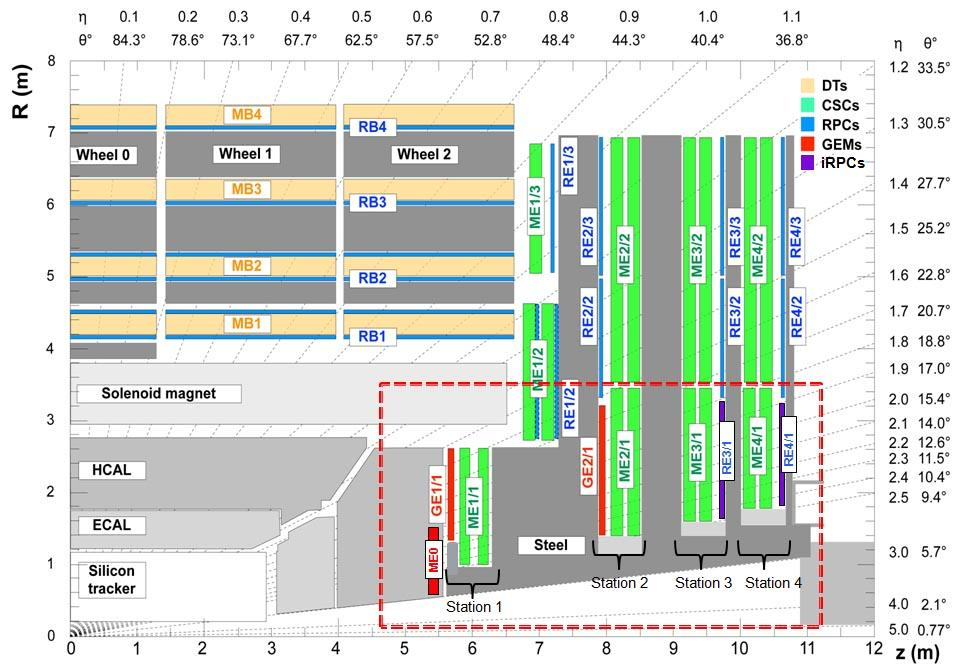
\includegraphics[width=0.7\textwidth]{fig/MuonUpgrade-Plans.jpg}
	\caption{\label{fig:Quadrant} A quadrant of the muon system, showing \acsp{DT} (yellow), \acsp{RPC} (light blue), and \acsp{CSC} (green). The locations of new forward muon detectors for Phase-II are contained within the dashed box and indicated in red for \acs{GEM} stations (\acs{ME0}, \acs{GE1/1}, and \acs{GE2/1}) and dark blue for improved RPC (\acs{iRPC}) stations (RE3/1 and RE4/1).}
\end{figure}

\acsp{RPC} are used by the \acs{CMS} first level trigger for their good timing performances. Indeed, a very good bunch crossing identification can be obtained with the present \acs{CMS} \acs{RPC} system, given their fast response of the order of \SI{1}{ns}. In order to contribute to the precision of muon momentum measurements, muon chambers should have a spatial resolution less or comparable to the contribution of multiple scattering~\cite{MUONTDR}. Most of the plausible physics is covered only considering muons with $p_T<$\SI{100}{GeV} thus, in order to match \acs{CMS} requirements, a spatial resolution of $\mathcal{O}$(few $\mathrm{mm}$) the proposed new \acs{RPC} stations, as shown by the simulation in figure~\ref{fig:MultiScat}. According to preliminary designs, \acs{RE3/1} and \acs{RE4/1} readout pitch will be comprised between 3 and \SI{6}{mm} and 5 $\eta$-partitions could be considered.

\begin{figure}[ht!]
	\centering
	\includegraphics[width=0.6\textwidth]{fig/MS_allstations.pdf}
	\caption{\label{fig:MultiScat}  \acs{RMS} of the multiple scattering displacement as a function of muon $p_T$ for the  proposed forward muon stations. All of the electromagnetic processes such as bremsstrahlung and magnetic field effect are included in the simulation.}
\end{figure}

\clearpage{\pagestyle{empty}\cleardoublepage}

% Header
\renewcommand\evenpagerightmark{{\scshape\small Chapter 3}}
\renewcommand\oddpageleftmark{{\scshape\small Muon Phase-II Upgrade}}

\renewcommand{\bibname}{References}

\hyphenation{}

\chapter[Muon Phase-II Upgrade]%
{Muon Phase-II Upgrade}
\label{chapt:3}
		
	The very first proton beam successfully circulated in the LHC in September 2008 directly followed by an incident leading to mechanical damage that would delay the LHC program for a year until November 2009, the very first collisions at a center-of-mass energy of \SI{7}{TeV} taking place in March 2010. The energy of the beam would be increased after a \acf{LS1} starting early 2013 after less than 3 years of data taking. Nevertheless, this first data taking period at only \SI{7}{TeV} was sufficient to claim the discovery of a new particle compatible with the Higgs boson in July 2012. During the 2 years of shutdown, the upgrade of the accelerator allowed for several maintainances along the beam pipes, repair and consolidation of magnet connection and high-current splices. But not only the LHC was upgraded. Indeed, the experiments at the 4 collision points also took the advantage of this time to upgrade their system in prevision of the next LHC run (Run-II) until 2018 and the \acf{LS2} as the luminosity and energy of the beam would be continuously increasing. By the end of Run-II, the luminosity will have reached twice its nominal value when the center-of-mass energy has already got close to its nominal value by reaching an historical \SI{13}{TeV} for the first time in 2017.
	
	The next long shutdown will occur at the end of this year and will again be the occasion for similar maintenance and consolidation in prevision of Run-III and the future upgrade of LS3. Still, the main occupation of LS2 on LHC side will be the upgrade of LHC injectors. On the experiments side, LHCb and ALICE will, in a very tight schedule, implement major upgrades while ATLAS and CMS will wait until LS3 to upgrade their detectors in prevision of high luminosity \textit{LHC-Phase-II}. ALICE main challenge is an upgrade of their apparatus to cope with the \SI{50}{kHz} $Pb-Pb$ collisions. Similarly, LHCb will upgrade their frontend readout electronics to cope with the full \SI{40}{MHz} collisions delivered by LHC. ATLAS will perform standard maintenance and CMS will focus on the urgent upgrade of the pixel detector and on the installation of new muon detectors in order to take profit of LS2 time to mitigate the upgrade of detectors forseen during LS3. Run-III will start in 2021 with the LHC at its nominal center-of-mass energy and will bring LHC-Phase-I to an end at the end of 2023. By then the luminosity will only increase to reach 2.5 times the nominal luminosity but during these 3 years of run, the LHC will deliver as much integrated luminosity as what what brought during the almost 7 years of both Run-I and II of data taking. Phase-I will end with an overall \SI{300}{fb^{-1}} delivered.\\
	
\section{\acl{HL-LHC} and muon system requirements}
\label{chapt3:sec:requirements}
	
	\begin{figure}[H]
		\begin{subfigure}{\linewidth}
			\centering
			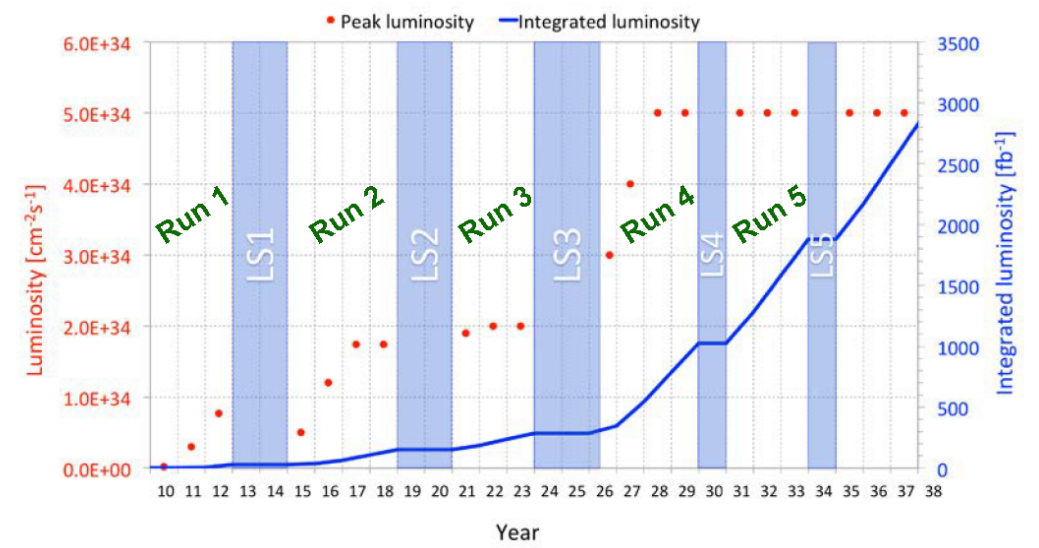
\includegraphics[width=\plotwidth]{fig/chapt3/HL-LHC-nominal.png}\\
			\caption{\label{fig:HL-LHC-Timeline:A}}
		\end{subfigure}
		\begin{subfigure}{\linewidth}
			\centering
			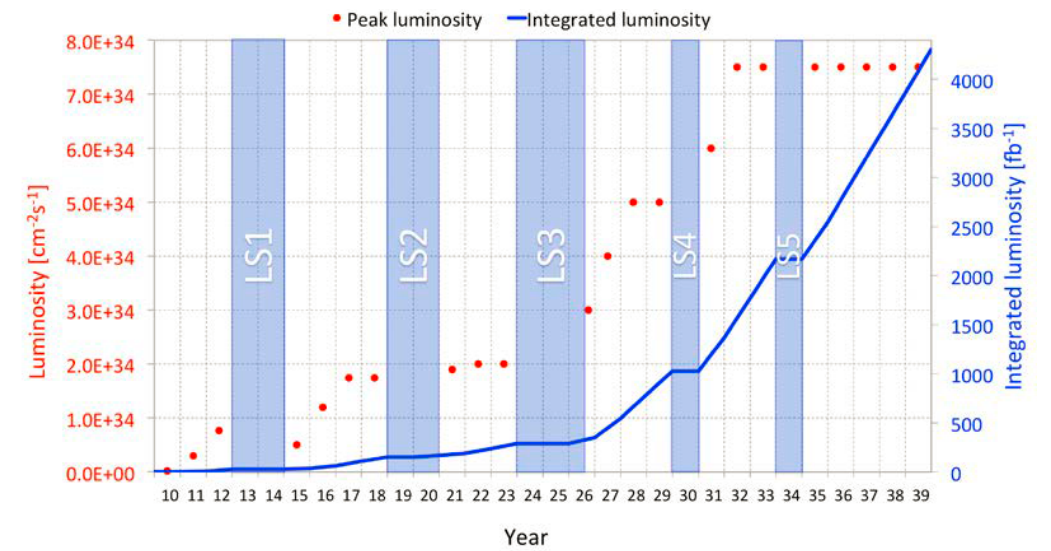
\includegraphics[width=\plotwidth]{fig/chapt3/HL-LHC-ultimate.png}
			\caption{\label{fig:HL-LHC-Timeline:B}}
		\end{subfigure}
		\caption{\label{fig:HL-LHC-Timeline} Detailed timeline projection of for LHC and HL-LHC operation until 2039 showing the evolution of the instanteneous and integrated luminosity as designed (Figure~\ref{fig:HL-LHC-Timeline:A}) and in the ultimate case where the instantaneous luminosity is increased to $7.5\times10^{34}$ \si{cm^{-2}s^{-1}} (Figure~\ref{fig:HL-LHC-Timeline:B})~\cite{HLLHC2017,HLLHCPDR}.}
	\end{figure}
		
	After approximately 15 years of operation, the LHC will undergo a new series of upgrade during the LS3 in order to boost its discovery potential as showed in Figure~\ref{fig:HL-LHC-Timeline}. This moment onward is what is referred to HL-LHC or Phase-II. The goal is to aim for a luminosity 5 to 7 times stronger than the nominal one trying to reach even 10 times this value if possible. Increasing the luminosity means that the beam size at the collision points needs to be reduced to boost the number of collisions per bunch crossing. For this purpose, new focusing and bending magnets, and collimators will be installed at the collision points as well as newly developed \textit{"crab cavities"} that will tilt the particle bunches just prior to the collisions by giving them transverse momentum and thus increasing their meeting area. In addition, the full proton injection line will be upgraded.
	
	Over its full lifetime, the HL-LHC is expected to deliver an outstanding integrated luminosity of \SI{3000}{fb^{-1}} leading, in the case of Higgs studies to measuring the couplings of the boson to a precision of 2 to 5\% thanks to the estimated 15 millions of Higgs created every year providing a more precise measurement of potential deviations from the theoretical predictions. SUSY and heavy gauge boson studies would also see their mass range limits pushed away by at least \SI{1}{TeV} and could lead to a new breakthrough. SUSY is a particularly important topic as it could give an answer to why the Higgs boson can stay so light while coupled to heavy particles by introducing the contributions of the super partners on top of providing dark matter candidates. Finally, the increase of luminosity will give the possibility to investigate "exotic" mode like for example the models introducing extra dimensions to explain the hierarchy problem.
	
	On the experiments side, the \acf{PU} will be increased up to 150 to 200 interactions per bunch crossing in ATLAS and CMS, making necessary an strong upgrade of the trigger system and of the inner trackers and of the calorimeters. Both ATLAS and CMS will also need to upgrade the muon trigger at the level of the endcaps mainly focusing on the coverage near the beam line in order to increase the detection acceptance and event selection. Moreover, the increased luminosity will also lead to an increased background rate and a faster ageing of the detectors. This PhD work takes place into this very specific context of muon detector consolidation and certification for the HL-LHC period in order to provide the CMS experiment with robust new detectors and confirm that the present system will survive through the next 20 years of HL-LHC.

	\begin{figure}[H]
		\centering
		\includegraphics[width=0.7\textwidth]{fig/chapt3/HL-LHC-Dose.png}
		\caption{\label{fig:Dose} Absorbed dose in the CMS cavern after an integrated luminosity of \SI{3000}{\femto\per\barn}. Using the interaction point as reference, R is the transverse distance from the beamline and Z is the distance along the beamline.}
	\end{figure}

	The end of 2018 will mark the beginning of LS2 and the start of Phase-II upgrade activities. From the HL-LHC period onwards, i.e. past LS3, the performance degradation due to integrated radiation as well as the average number of inelastic collisions per bunch crossing, seen as pile-up into the detectors' readout that far exceeds this of the original LHC plans, will rise substantially and become a major challenge for all of the LHC experiments, like CMS, that were forced to address an upgrade program for Phase-II~\cite{PHASEIITP}. Dealing with the data from the muon detectors will force to upgrade the detectors and electronics towards the most recent technologies. Simultaneously, this will push new latency requirements onto the Level-1 trigger and the \acf{DAQ} that will only be fulfilled by upgrading the system with electronics having deeper buffering and faster processing. Simulations of the expected distribution of absorbed dose in the CMS detector under HL-LHC conditions show, in Figure~\ref{fig:Dose}, that detectors placed close to the beam line will have to withstand high irradiation, the radiation dose being of the order of a few tens of \si{Gy}.
	
	\begin{figure}[H]
		\centering
		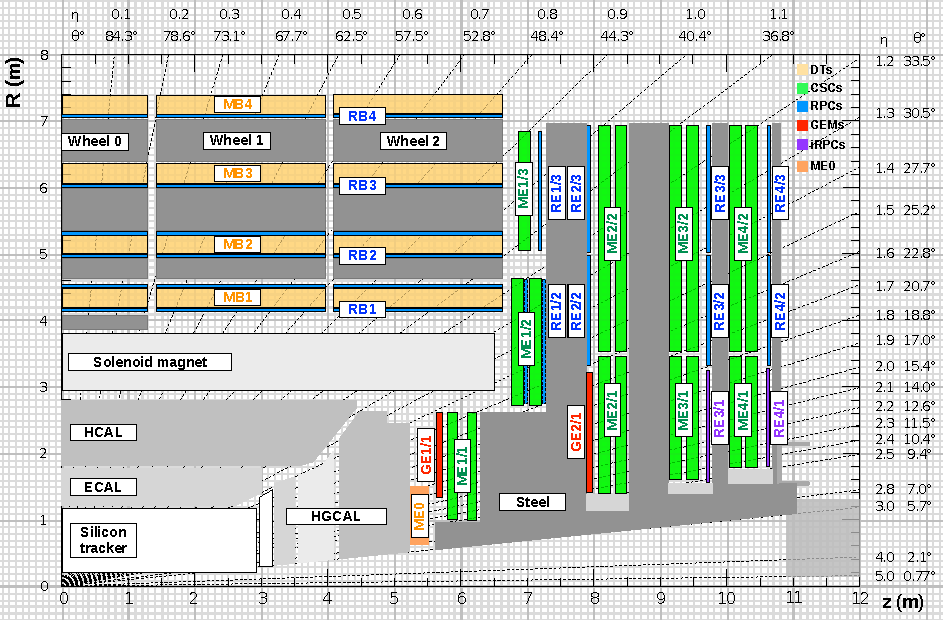
\includegraphics[width=0.7\textwidth]{fig/chapt3/Phase2_Muon_quadrant.pdf}
		\caption{\label{fig:P2Quadrant} A quadrant of the muon system, showing DTs (yellow), RPCs (blue), and CSCs (green). The locations of new forward muon detectors for Phase-II are contained within the dashed box and indicated in red for GEM stations (ME0, GE1/1, and GE2/1) and dark blue for improved RPC (iRPC) stations (RE3/1 and RE4/1).}
	\end{figure}

	The increase of irradiation close to the beam line will affect the background rate seen by the muon detectors in this area and tracking muons will prove to be difficult as this region is not yet equipped with all the detectors that were already foreseen for Phase-I. Improving this situation will come with the increase of hit numbers recorded along the particle track to reduce the ambiguity on muon versus background detection. Moreover, the measurement of small production cross-section and/or decay branching ratio processes, such as the Higgs boson coupling to charge leptons, and in particular to muons, or the $B_s \longrightarrow \mu^+\mu^-$ decay, is of major interest and specific upgrades in the forward regions of the detector will be required to maximize the physics acceptance to the largest possible solid angle.
	
To ensure proper trigger performance within the present coverage, the muon system will be completed with new chambers and the electronics of the present system will need to be upgraded to ensure an efficient triggering. Figure~\ref{fig:P2Quadrant} shows the addition of \acf{GEM} and \acf{iRPC} in the pseudo-rapidity region $1.6<\vert\eta\vert<2.4$ to complete the redundancy of the already existing CSCs as originally scheduled in the CMS Technical Proposal~\cite{CMSTP}. A first step into this direction will be taken by installing GEMs on the first endcap disk in position GE1/1 during LS2, during which preparations for the future installation of more GEMs and RPCs will take place by installing the needed services. During the YETS following LS2, iRPCs will be installed on the third and fourth endcap disks in position RE3/1 and RE4/1, and more GEMs will equip the second endcap in position GE2/1 and the inner layer, closest to the HCAL endcap called ME0 during LS3, finally completing the redundant coverage of the muon system and extending it a little by extending the reach to \psrape{2.8}, the redundancy in the region \psrapr{2.4}{2.8} being maintained by the 6 GEM layers contained in each ME0 detector that provide enough tracking points to efficiently reject neutron-induced background.
	
	Nevertheless, the region beyond \psrapg{2.8} and extending to \psrape{5.0} only is covered by the forward HCAL detectors and lack redundant muon detector coverage. Extensions of the tracker in the context of HL-LHC will increase its coverage up to \psrape{4.0} but the identification of muons and measurement of their energy with reasonable precision only using the tracker is nearly impossible. Thus, this increased tracker coverage range needs to be put in parallel with a matching muon detector and will open doors to multi-lepton final states in which leptons are likely to have a a low transverse momentum and to be found near the beam line.\\
	
	Finally, as the muon system is composed only of gaseous detectors, strong environmental concerns have risen over the last years as the European directives will restrict the use of fluorine based gas mixtures. Both the CSC and RPC subsystems, using $CF_4$, $C_2H_2F_4$, or $SF_6$, will need to adapt their working gas in order to strongly reduce the greenhouse potential of the mixtures released into the atmosphere due to gas leaks.
	
\section{Necessity for improved electronics}
\label{chapt3:sec:electronics}

	Drift Tubes and Cathode Strip Chambers are important components used to identify and measure muons, especially thanks to their spatial resolution of the order of \SI{100}{\micro m}. Nevertheless, the luminosity and irradiation during HL-LHC will cause serious event loss and ageing on the electronics of these subsystems that will comprise the triggering and data transfering needs of CMS. Thus, electronics upgrade are foreseen to address these expected problems. While only the RPCs' electronic system is able to operate under Phase-II requirements, DTs and CSCs will need to improve their trigger accept rate and latency to ensure that Level-1 trigger threshold stays at the same level~\cite{LEVEL1IR}, and DAQ data transfer rate, that respectively need to achieve a minimum of \SI{500}{kHz}, get down to \SI{12.5}{\micro s}~\cite{CMSIITP}, and increase to \SI{1082}{Gbit/s} DTs and to \SI{1026}{Gbit/s} for CSCs. As of today, the Level-1 trigger accept rate of DTs doesn't reach \SI{300}{kHz} while this of CSCs is bellow \SI{250}{kHz} but the foreseen upgrades are expected to increase the rate way beyond the requirement in the of DTs and up to \SI{4}{MHz} for CSCs~\cite{PHASEIITP}.
	
	The \acf{MiC1} used by DTs don't allow for high enough trigger rate. In addition to this problem, it was showed that these electronics contain components that are not radiation hard enough to sustain HL-LHC conditions and thus, a too large number of channels may fail due to radiations. Considering the most optimistic scenario, at least 19\% of the channels could have failed by LS4, as explicited in Figure~\ref{fig:DT-upgrade}, far before the end of the HL-LHC campain. The MiC1 will be replaced on each detector by an improved version referred to as MiC2 while front-end electronics and high-voltage modules will not need any replacement. On the other hand, CSCs showed that there electronics would be able to live through the 10 years of Phase-II but the limited buffer depth might cause memory overflows and readout inefficiencies with a fraction of event loss ranging from 5 to more than 10\% at an instantaneous luminosity similar to which of HL-LHC depending on the expected background, as showed on Figure~\ref{fig:CSC-upgrade} through the different detector positions. Thus the replacement of CSCs' \acf{CFEBs} by digital ones, DCFEBs, with deeper buffer would permit to make event loss negligible and satisfy HL-LHC requirements~\cite{PHASEIITP}.
	
	\begin{figure}[H]
		\begin{subfigure}{\linewidth}
			\centering
			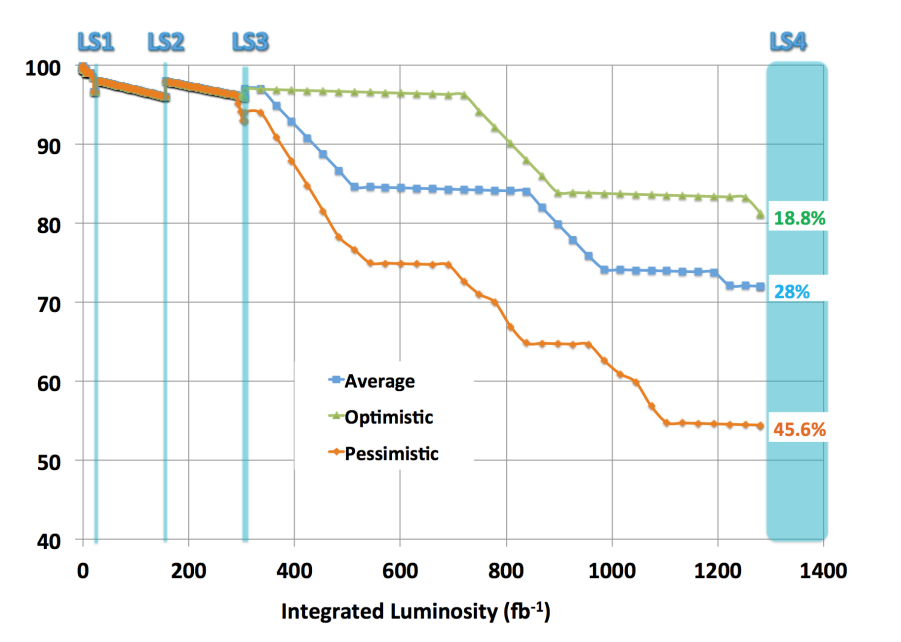
\includegraphics[width=0.8\plotwidth]{fig/chapt3/DT-channel-failure.png}\\
			\caption{\label{fig:DT-upgrade:A}}
			
		\end{subfigure}
		\begin{subfigure}{\linewidth}
			\centering
			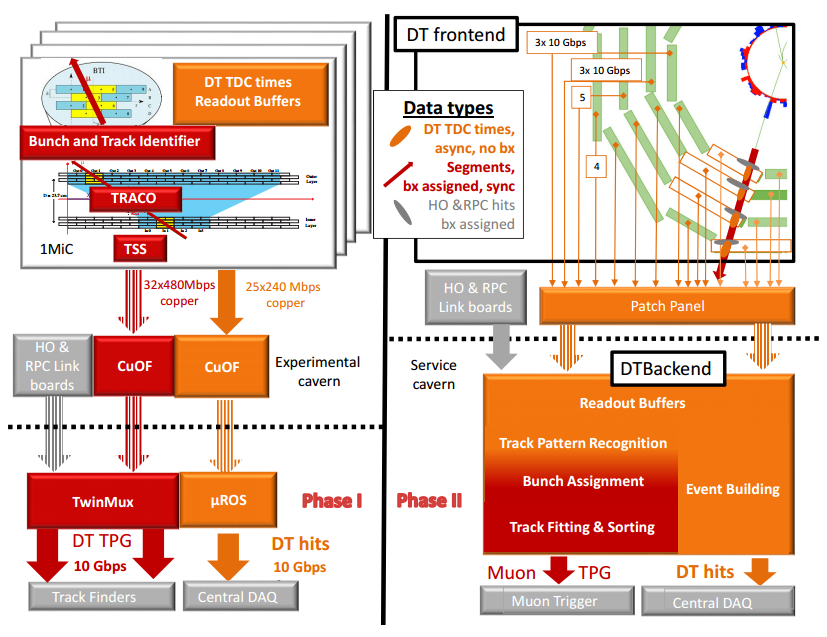
\includegraphics[width=0.9\plotwidth]{fig/chapt3/DT-upgrade.png}
			\caption{\label{fig:DT-upgrade:B}}
		\end{subfigure}
		\caption{\label{fig:DT-upgrade} Figure~\ref{fig:DT-upgrade:A}: Extrapolated fraction of failing channels of the present DT MiC1 electronics as a function of the integrated luminosity for different scenari until LS4. Figure~\ref{fig:DT-upgrade:B}: Comparison of the current (left) and upgraded (right) DT data processing. So far, the data is sent to service cavern of CMS facility via copper-to-optical-fiber translators (CuOF) by each MiC1. There, data including RPCs and outer hadron calorimeter is combined into trigger primitives (TPG) and transmitted by the TwinMux system to CMS Track Finder. The time-to-digital converter (TDC) data is collected and sent to the CMS data acquisition system (DAQ) by the micro read-out server ($\mu$ROS). After the upgrade, the TDC data will be sent via optical links to a patch panel inside the experimental cavern by each MiC2, and transferred to the back-end, where triggering and event building will be performed.}
	\end{figure}
	
	\begin{figure}[H]
		\begin{subfigure}{\linewidth}
			\centering
			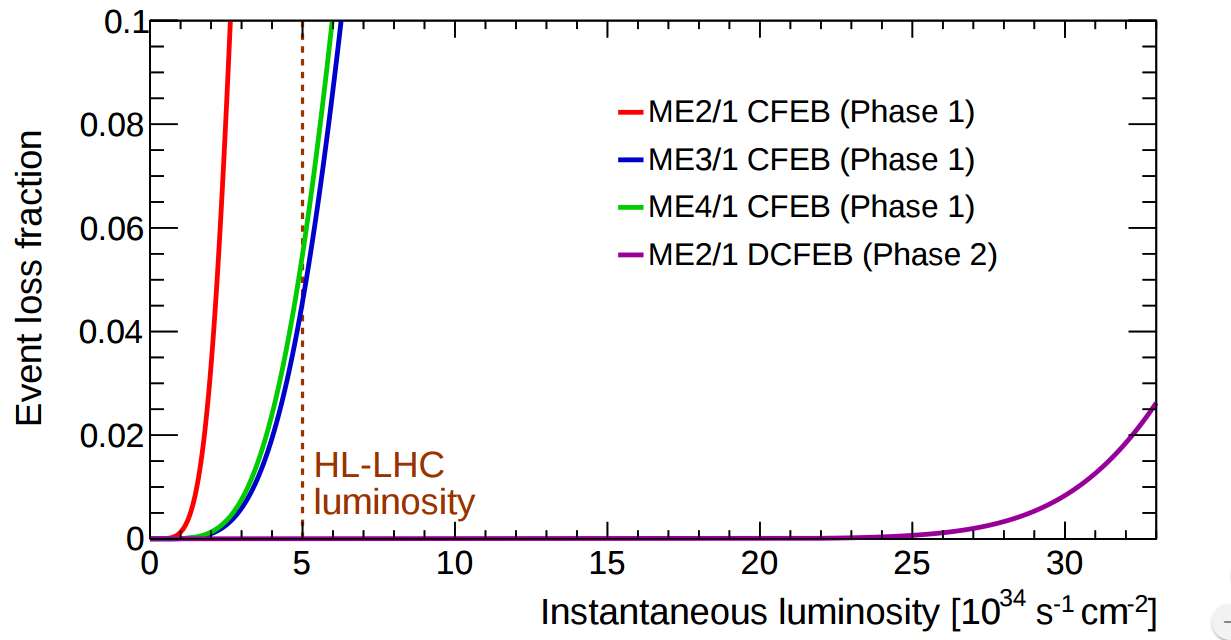
\includegraphics[width=\plotwidth]{fig/chapt3/CSC-event-loss.png}\\
			\caption{\label{fig:CSC-upgrade:A}}
		\end{subfigure}
		\begin{subfigure}{\linewidth}
			\centering
			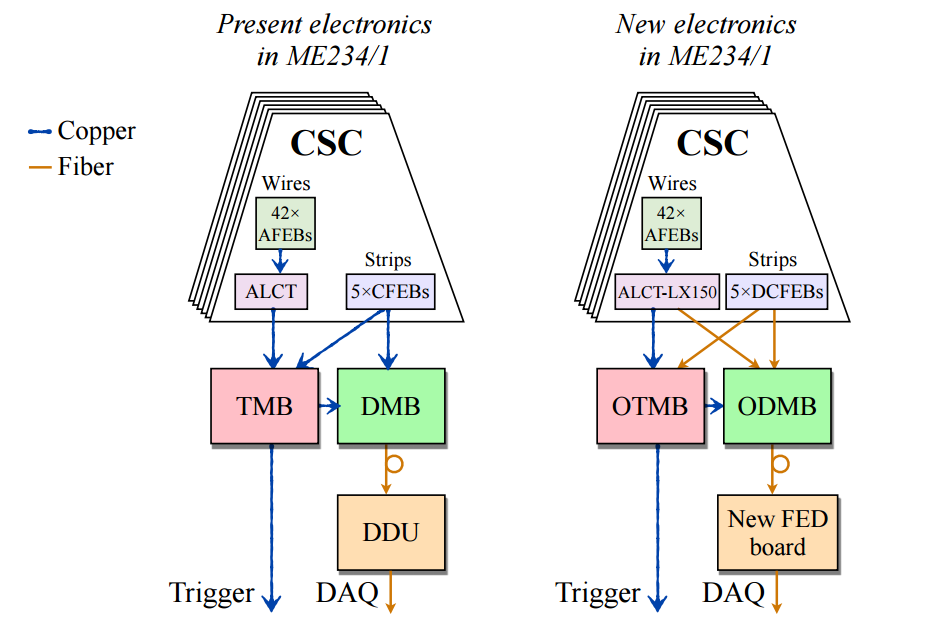
\includegraphics[width=\plotwidth]{fig/chapt3/CSC-upgrade.png}
			\caption{\label{fig:CSC-upgrade:B}}
		\end{subfigure}
		\caption{\label{fig:CSC-upgrade} Figure~\ref{fig:CSC-upgrade:A}: The event loss fractions as a function of the instantaneous luminosity is compared for CFEBs (Phase-1) and DCFEBs (Phase-II) at different CSC locations. HL-LHC luminosity is marked with the dashed brown line. Figure~\ref{fig:CSC-upgrade:B}: Comparison of the current (left) and upgraded (right) CSC data processing. A part of the connections in between ALCTs and DCFEBs, and the trigger mother boards (TMBs) and data acquisition mother boards (DMBs) will be upgraded toward optical data transfer. The detector dependent units (DDUs) used as interface in betweend CSCs' front-end electronics and the CMS DAQ will be replaced by new FED boards.}
	\end{figure}
	
	All these new DT and CSC electronics will be connected to the trigger electronics via optical links to ensure a faster communication. The main change will come from the new DT minicrate modules which will not anymore be responsible for trigger and event building logic which will be transfered to the back-end electronics instead located in the service cavern via the patch pannels to which the \acf{TDC} data will be sent. The trigger and data transfer logic will barely change for CSCs. The existing copper cable connections of cathode and anode FEBs (CFEBs, and AFEBs which data is transmitted through the ALCTs) toward the trigger and data mother boards (TMBs and DMBs) will simply be replaced by optical fibers and the TMBs and DMBs upgraded with optical versions (OTMBS and ODMBs). As a new feature, the full anode wire data from ALCTs will be sent to the ODMBs causing a lack of FPGA memory resources in these ALCT boards that will thus need replacement.
	
	\begin{figure}[H]
		\centering
		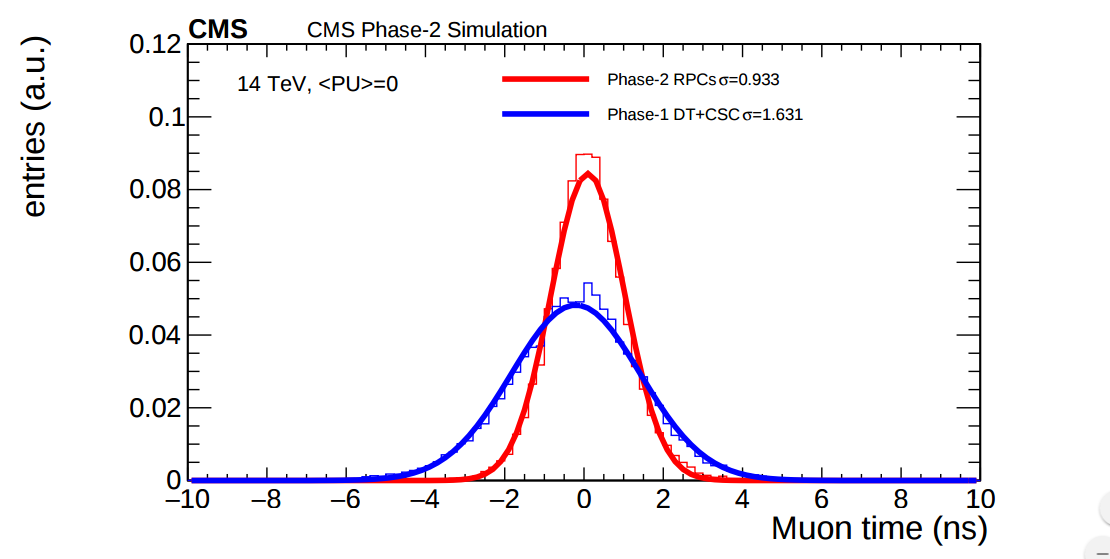
\includegraphics[width=\plotwidth]{fig/chapt3/RPC-ugrade-LS.png}
		\caption{\label{fig:RPC-time} Comparison of the simulated time residuals in between reconstructed and true muon times without (blue) and with (red) the upgraded RPC link system.}
	\end{figure}
	
	The upgrade on the side of Resistive Plate Chambers will then not come from their on-board electronics but from the Link System located in the service cavern of CMS and that connects the front-end electronics data of RPCs into CMS trigger processors. The main motivation for such and upgrade is that the electronic board composing the link system are built using obsolete components and weak components that can easily suffer from the electromagnetic noise. These components may be the source of failing channels throughout Phase-II. Moreover, these link boards were originally designed only to match RPC digitized signals with the corresponding bunch crossing. Due to this feature, the time resolution of the full RPC chain is thus limited to \SI{25}{ns} and does not exploit the full time resolution of the detectors. This would make the synchronization of the RPC system easier and allow to have a finer offline background removal within the \SI{25}{ns} in between bunch crossings thanks to the order of magnitude gained in terms of time resolution.
	
	Upgrading RPC link system will require the installation of 1376 new link boards and 216 control boards. The new boards will make use of the recent progress made with fast FPGAs and will be a great improvement to the ASICs formerly used as they will be able to process signals from several detectors in parallel. The benefice from using the full RPC time resolution thanks to the upgraded link system can be seen through Figure~\ref{fig:RPC-time} where the resolution of the RPC system itself is better than which of DTs and CSCs that was used until now.

\section{New detectors and increased acceptance}
\label{chapt3:sec:GEMRPC}

	In the present muon system, the redundancy of was assured by RPCs used for their good timing performances. The extension of the muon system towards higher pseudo-rapidity in order to complete the redundancy in this very region and to contribute to the precision of muon momentum measurements will require muon chambers with a spatial resolution less or comparable to the contribution  muon of multiple scattering through the detector volume~\cite{MUONTDR}. Most of the plausible physics is covered only considering muons with $p_T<$\SI{100}{GeV} thus, in order to match CMS requirements, a spatial resolution of $\mathcal{O}$(few $\mathrm{mm}$) will be necessary for the proposed new RPC stations while the GEMs will need a resolution better than \SI{1}{mm}, as showed by the simulation in Figure~\ref{fig:MultiScat}.

	\begin{figure}[H]
		\centering
		\includegraphics[width=0.6\textwidth]{fig/chapt3/MS_allstations.pdf}
		\caption{\label{fig:MultiScat} RMS of the multiple scattering displacement as a function of muon $p_T$ for the proposed forward muon stations. All of the electromagnetic processes such as bremsstrahlung and magnetic field effect are included in the simulation.}
	\end{figure}
	
	\subsection{Improved forward resistive plate chambers}
	\label{chapt3:ssec:iRPCs}

	\begin{figure}[H]
		\centering
		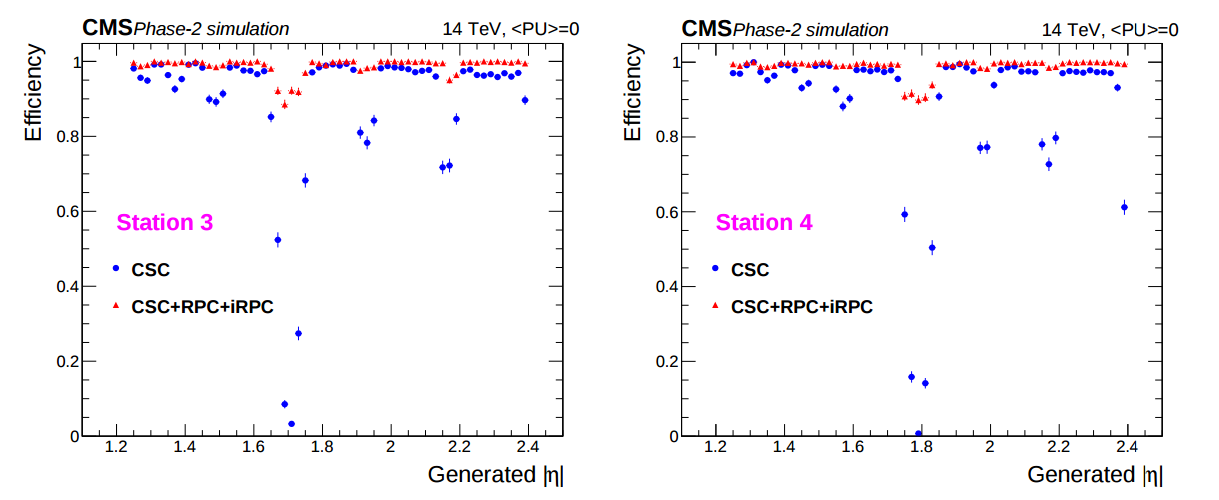
\includegraphics[width=\linewidth]{fig/chapt3/Trigger-efficiency-endcap.png}
		\caption{\label{fig:Endcap-trigger-eff} Simulation of the impact of RPC hit inclusion onto the local trigger primitive efficiency in station 3 (left) and station 4 (right). The contribution of iRPC starts above \psrape{1.8}.}
	\end{figure}
	
	Figure~\ref{fig:P2Quadrant} shows that the iRPCs that will equip the third and fourth endcap disks in position RE3/1 and RE4/1 will finally be the partners of the CSCs in position ME3/1 and ME4/1 and complete Phase-I plans but bringing the needed upgrades in the scope of Phase-II as the older chambers are not suitable to equip the forward region of CMS due to HL-LHC rates and charge deposition. By completing the redundancy, more track along the muon trajectory will be available and the lever arm will be improved. The benefits from extending the redundancy of the muon system with iRPCs to the forward most region is showed in Figure~\ref{fig:Endcap-trigger-eff} in which the trigger efficiency is showed with and without RPCs in which it is possible to see that the efficiency of CMS trigger with the complete redundancy is improved is above 95\% in the region \psrapg{1.8} as the iRPCs help filling the holes in the CSC system.\\
	
	The detectors that will be installed in the coming years will be similar to the already existing RPC system. 18 of the new chambers, each spanning \SI{20}{\degree} in $\varphi$ around the beam axis with 96 radially oriented trapezoidal read-out strips, will cover each muon endcap disk leading to the production of 72 iRPCs.The main difference with the old RPC chambers is that these detectors will not have readout strips segmented in $\eta$ as by using fast front-end electronics the strips will be read-out on both sides allowing for a radial spatial resolution of the order of \SI{2}{cm} in order to contribute to the better reconstruction of muon in the forward region where the bending of muons by the magnetic field is low. This is motivated by the fact that, in the case a $\eta$ segmentation was used, at least 5 pseudorapidity partitions would have been necessary to reach the minimal radial spatial resolution ($\approx$ \SI{20}{cm}). Having only one strip read-out from both along the chamber reduces by 60\% the total number of channels and the necessary cabling and allows for a better spatial resolution. The strip pitch will range from \SI{6.0}{mm} (\SI{5.9}{mm}) on the high pseudo-rapidity end to \SI{12.3}{mm} (\SI{10.9}{mm}) on the low one on position RE3/1 (RE4/1). The spatial resolution in the direction perpendicular to the strips should reach approximately \SI{3}{mm}, better than the minimal needed resolution (Figure~\ref{fig:MultiScat}), and the overall time resolution of the new installation will be equally \SI{1.5}{ns}, as for the present due to the same link system being used.

	\begin{figure}[H]
		\centering
		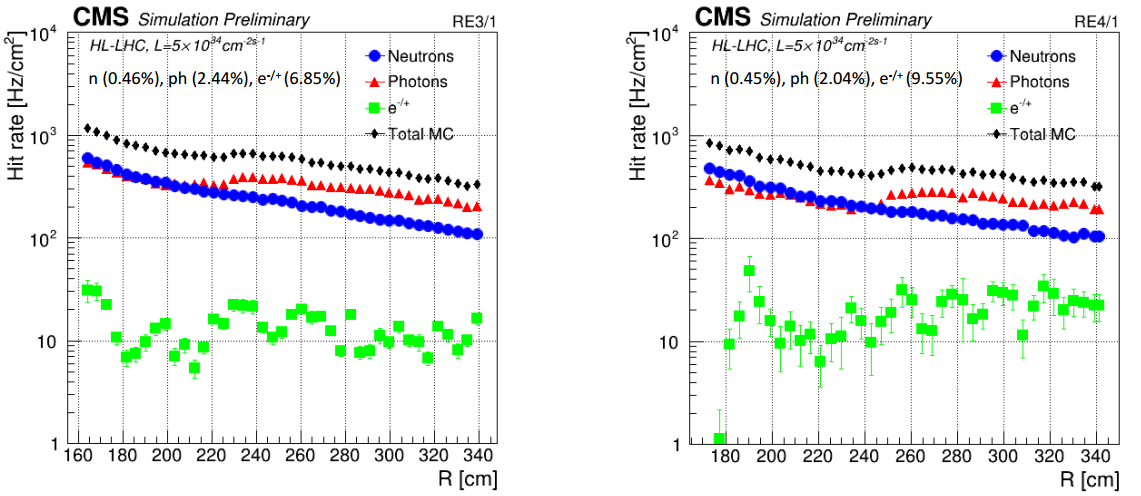
\includegraphics[width=\textwidth]{fig/chapt3/RPC-Sim-HL-LHC_Rate.png}
		\caption{\label{fig:iRPC-Rate} Expected hit rate due to neutrons, photons, electrons and positrons at HL-HLC instantaneous luminosity of $5\times10^{34}$ \si{cm^{-2}s^{-1}} in RE3/1 and RE4/1 chambers. The sensitivities of iRPCs used in the simulation for each particle are reported and differ from one endcap disk to another as the energies of the considered particles varies with the increasing distance from the interaction point.}
	\end{figure}
	
	Nevertheless, having only a single strip instead of pseudo-rapidity segmentation will increase the probability of double hits in the same channel. This probability was estimated to be low enough as it shouldn't exceed 0.7\%. This estimation was made assuming an average hit rate per unit area of \SI{600}{Hz/cm^2} in the iRPCs (see Figure~\ref{fig:iRPC-Rate}), a cluster size (average number of strips fired per muon) of 2, a strip active area of \SIsurface{158.4}{0.87}{cm} and a safety factor 3 leading to an estimated rate per strip of \SI{380}{kHz} corresponding to an average time interval of \SI{2600}{ns} in between 2 consecutive hits. The time for a signal to go through the full strip length is about \SI{10}{ns} to which can be added \SI{1}{ns} of dead time and 2 TDC clock cycles of \SI{2.5}{ns} for a minimal time interval of \SI{16}{ns} necessary to avoid ambiguities. The probability of having ambiguous double hits in a strip in then the ratio in between this minimal time interval in between 2 consecutive hits and the average time interval estimated from the rate the detectors are subjected to.
	
	The instantaneous luminosity at HL-LHC being very high, the rates at the level of the new chambers needed to be simulated in order to understand the necessary requirements for these detectors. The simulated results for different background components (neutrons, photons, electrons and positrons) are showed in Figure~\ref{fig:iRPC-Rate} assuming known sensitivities to these particles. It is showed that on average over the iRPC areas the rates would be of the order of \SI{600}{Hz/cm^2} (\SI{600}{Hz/cm^2} seen in RE3/1 and \SI{480}{Hz/cm^2} in RE4/1)~\cite{ANDREA2018}. Thus, taking into account a safety factor of about 3, it was decided that improved RPCs should at least be certified for rates reaching \SI{2}{kHz/cm^2} which would be achieved thanks to several improvements on the design and on the electronics. The detectors design will be based on the existing RPC design as they will be double gaps. Similarly to the existing RPC system, the electrode material will be HPL although the thickness of the electrodes and of the gas gap will be reduced to \SI{1.4}{mm} as a thinner gas gap leads to a decrease of deposited charge per avalanche as showed in Figure~\ref{fig:charge-gap}. The smaller the gas gap, the more the detector becomes sensitive to gap non-uniformities across the electrode planes making a gap of \SI{1.4}{mm} a good compromise in between these two competing factors.

	\begin{figure}[H]
		\centering
		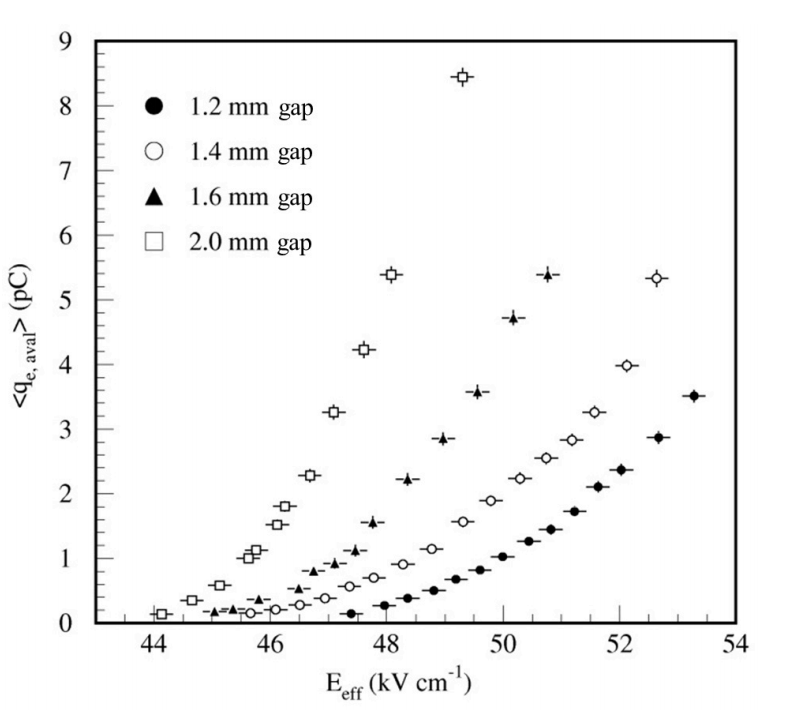
\includegraphics[width=0.8\plotwidth]{fig/chapt3/charge-vs-gap.png}
		\caption{\label{fig:charge-gap} Measured average charge per avalanche as a function of the effective electric field for different gas gap thickness in double gap RPCs using HPL electrodes.}
	\end{figure}

	\begin{figure}[H]
		\centering
		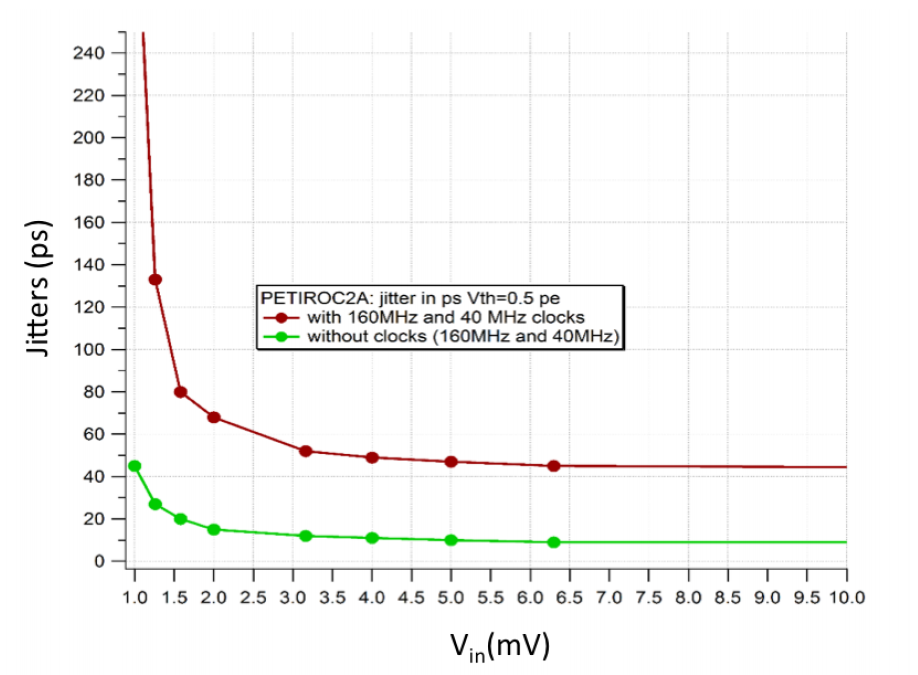
\includegraphics[width=0.8\plotwidth]{fig/chapt3/jitter-PETIROC.png}
		\caption{\label{fig:jitter} The PETIROC time jitter as a function of the input signal amplitude, measured with and without internal clocks.}
	\end{figure}
	
	A lower charge deposition inside of the detector volume means a slower ageing and a longer lifetime for detectors subjected to high irradiation. But, in order to take advantage of the lower detector gain, more sensitive electronics are required so that the part of gain that was formerly done in the gas volume can be moved to the electronics. Achieving this with the technology developed more than 10 years ago for the present system is not possible as the signal over noise ratio of such electronics doesn't allow to detect charges as low as \SI{10}{fC}. Moreover, the new front-end electronics will need to be radiation hard to survive to more than 10 years of HL-LHC conditions. The new technology that has been chosen is based on the PETIROC ASIC manufactured by OMEGA and is a 64-channel ASIC called CMS RPCROC on which the original SiGe technology will be replaced by CMOS to increase its radiation hardness while keeping fast pre-amplification and discrimination with a very low jitter that can reach less than \SI{20}{ps} if no internal clock is used, as can be seen from Figure~\ref{fig:jitter}. The ASIC is associated with an FPGA which purpose is to measure time thanks to a TDC with a time resolution of 50-100 \si{ps} developed by Tsinghua University and that will provide a measurement of the signal position along the strip with a precision of a few \si{cm} by measuring the signal timing on both ends of the strips. In order to read-out all 96 strips, 3 ASICs and 3 TDCs, each having 64 channels, are hosted on a front-end board attached to the chamber.\\
	
	{\color{blue}[Wait for the analysis of 2018 GIF++ data to add interesting information about the time and spatial resoltution measured during test beam periods.]\\}
	
	\subsection{Gas electron multipliers}
	\label{chapt3:ssec:GEMs}
	
	In the region closer to the interaction point where the spatial resolution is requested to be better than \SI{1}{mm} for the new detectors (at least for GE1/1 and ME0, GE2/1 being in the same order of requested spatial resolution than the new iRPCs that will equip the third and fourth endcaps), the choice has been made to use triple GEMs, micro pattern gaseous detectors, in the place of RPCs. The GE1/1 project had been the first to be approved and demonstrators had been installed in CMS already during LS1. The rest of the detectors will be installed during LS2 while the GE2/1 and ME0 projects are still under development. ME0, GE1/1 and GE2/1 will be installed respectively next to the HCAL endcap, on the first and on the second muon endcap disks as can be seen from Figure~\ref{fig:P2Quadrant}.

	\begin{figure}[H]
		\centering
		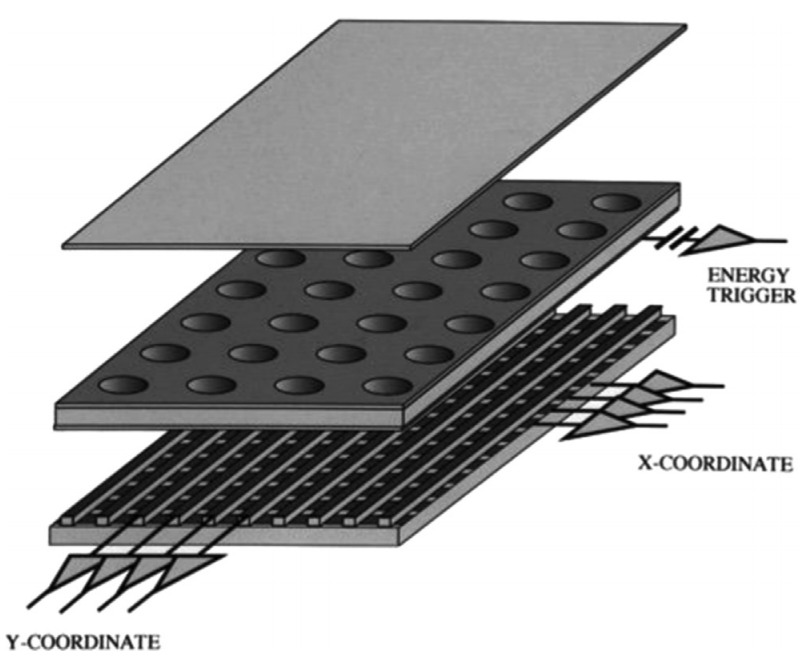
\includegraphics[width=0.7\plotwidth]{fig/chapt3/GEM.png}
		\caption{\label{fig:GEM} Schematics of a GEM showing the cathode on top, the GEM foil separating the gas volume into the drift region, in between the cathode and foil, and the induction region, in between the GEM foil and the anode, and the anode on which a 2D read-out is installed. A negative voltage is applied on the cathode while the anode is connected to the ground.}
	\end{figure}
	
	Gas Electron multipliers are gaseous detectors~\cite{SAULI97} which gas volume is confined in between 2 planar electrodes, the anode serving as read-out panel. The gas volume is divided in 2 or more regions by a single or multiple \textit{GEM foils} as showed in Figure~\ref{fig:GEM}. These foils are very thin, of the order of a few tens of \si{\micro m}, and are pierced with holes as can be seen in Figure~\ref{fig:GEM-foil}. Both surfaces of the GEM foils are clad with copper in order to apply a strong electric field in between each side that will generate very strong potentials in the holes. The gas region contained in between the cathode and the GEM foil is called the drift region as the electric field is not strong enough to cause avalanches and thus start an amplification. The primary electrons drift toward the foil and are accelerated and amplify by the very high potential within the holes, as showed in Figure~\ref{fig:GEM-foil}. Then the electrons reach the second drift region in which they will induce signal on the read-out located on the anode. By restraining the amplification process at the level of the holes, the electrons can stay in a very confined space and thus induce a very localized current, providing the GEMs with a very good spatial resolution.
	
	In order to achieve a stronger amplification, the amplification process can be repeated several times in a row. The GEMs that will be used in CMS are triple GEM detectors operated with a 70/30 gas mixture of $Ar$/$CO_2$. They contain 3 GEM foils and thus 3 electron amplifications, as can be seen in Figure~\ref{fig:GEM-drift}. The GEM foils used in CMS are \SI{50}{\micro m} foils clad with \SI{5}{\micro m} of copper on each side. The foils are pierced with double-canonical holes which inner and outer diameters are respectively 50 and \SI{70}{\micro m} which are placed \SI{140}{\micro m} from each other in an hexagonal pattern, as showed in Figure~\ref{fig:GEM-foil}. These detectors have a time resolution better than \SI{10}{ns} and reach very good spatial resolutions of less than \SI{200}{\micro rad} as indeed the position of the hits is not measured along the strips but following the azimuthal angle granularity of the radialy organized trapezoidal strips.

	\begin{figure}[H]
		\centering
		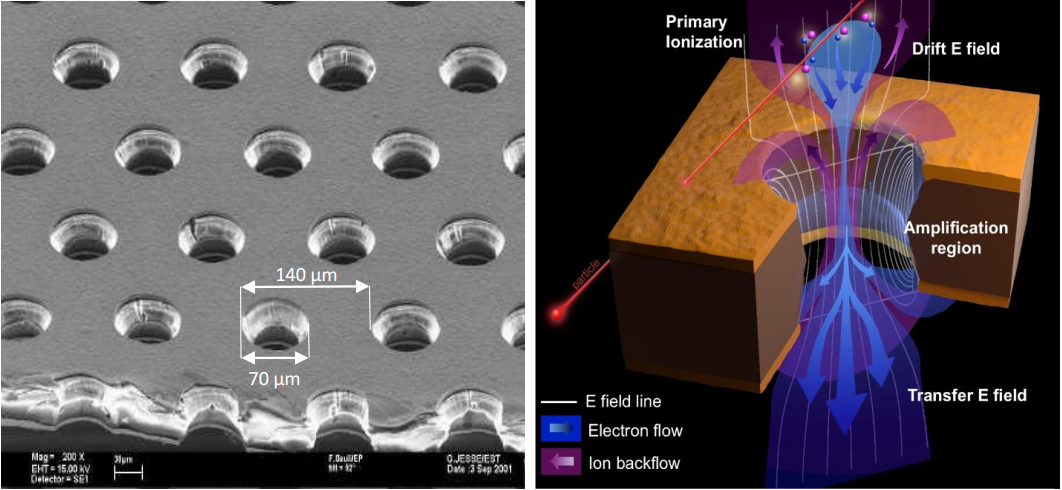
\includegraphics[width=\plotwidth]{fig/chapt3/GEM-foil-ampli.png}
		\caption{\label{fig:GEM-foil} Left: Picture of a CMS GEM foil provided by a scanning electron microscope. Righ: Representation of the electric field lines in a GEM hole and of the amplification that electrons and ions undergo in the hole's volume due to the very intense electric field.}
	\end{figure}

	\begin{figure}[H]
		\centering
		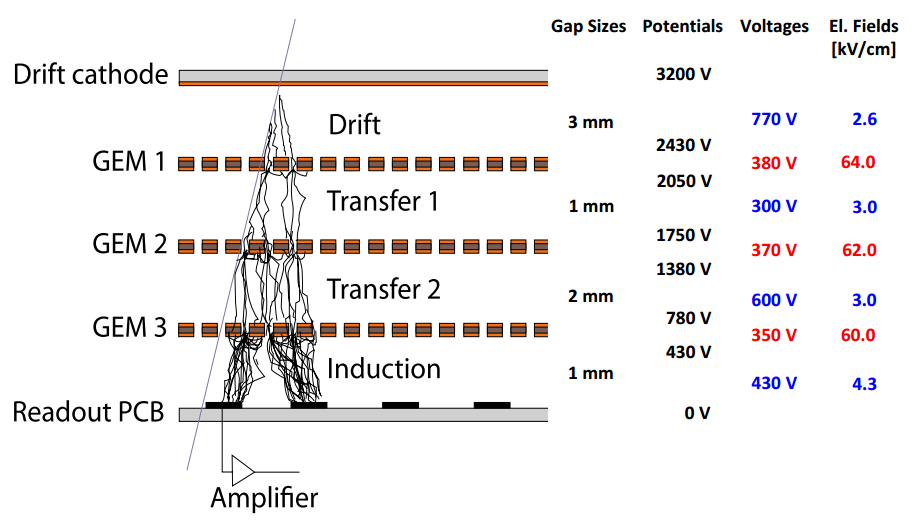
\includegraphics[width=\plotwidth]{fig/chapt3/GEM-drift.png}
		\caption{\label{fig:GEM-drift} Schematic representation of CMS triple GEMs. The gas volume is divided into 4 areas. The drift area is the region where the primary electrons are created before being amplified a first time while passing through the first GEM foil. Then the process of drift and amplification is repeated twice in following two transfer areas and GEM foils. Finally, the charges have been amplified enough to induce current in the read-out strips while in the last drift area. The dimensions, potentials and electric fields are provided.}
	\end{figure}
	
	The GEM Upgrade is divided into 3 subsystems as GE1/1 was the first approved project~\cite{GEM11TDR} and that the detectors will already be installed during LS2. GE2/1 and ME0, on the other hand, will profit of the R\&D knowledge and skills developed for GE1/1 while the requirements for each subsystem are different as they are not placed at the same distance from the interaction point. In this very forward region, a different position with respect to the center of the detector can change dramatically the conditions in which the detectors will have to be operated. In terms of rate capability, GE2/1, which is the furthest, is required to withstand \SI{2.1}{kHz/cm^2} while GE1/1 needs to be better than \SI{10}{kHz/cm^2} and ME), better than \SI{150}{kHz/cm^2}. In terms of ageing with respect to charge deposition, ME0 needs to be certified to \SI{840}{mC/cm^2}, GE1/1 to \SI{200}{mC/cm^2} and GE2/1 only to \SI{9}{mC/cm^2}. All 3 detectors need to have a time resolution better than \SI{10}{ns} and an angular resolution better than \SI{500}{\micro rad}.
	
	On each GE1/1 ring, 36 super chambers, consisting of 2 single GEM layers and spanning \SI{10}{\degree}, will be installed covering the pseudo-rapidity region \psrapr{1.6}{2.2} together with ME1/1 CSCs and the reach of the muon system will be improved thanks to the GE2/1 that will overlap with the GE1/1 and cover a region from \psrapg{1.6} to \psrapl{2.4} and complete the redundancy of ME2/1. The super chambers, built with 2 triple GEM layers each consisting of 4 single GEM modules due to the rather large surface of the GE2/1 chambers, that will be installed on the first ring of the second endcap will span \SI{20}{\degree} each, hence, a total of 72 chambers will be assembled to equip the muon system. Finally, the ME0 installed near the HCAl endcap will cover the region \psrapr{2.0}{2.8} and this subsystem will consist in super modules of 6 layers of triple GEM detectors covering an azimuthal angle of \SI{20}{\degree} leading to the construction of 216 single detectors.
	
	All these new GEM detectors will be using a similar internal layout which is described in Figure~\ref{fig:GEM-drift}. The incoming muons will create detectable electron-ion pairs in the \SI{3}{mm} thick drift volume in which an electric field of \SI{2.6}{kV/cm} is applied for the electrons to drift to the first GEM foil on which a very intense field of \SI{64}{kV/cm} is applied over a distance of only \SI{60}{\micro m} which allows for an average electronic gain of 20 to 25. After the first amplification stage, the electrons drift over the \SI{1}{mm} separating the 2 first GEM foils thanks to an electric field of \SI{3.0}{kV/cm} and are again amplified by a factor 20 to 25 while going through the second GEM foil to which is applied an electric field of \SI{62}{kV/cm}. The electron drift another \SI{2}{mm} towards the last GEM foil through a field of \SI{3.0}{kV/cm} and are multiplied one last time from a similar factor passing through the \SI{60}{kV/cm} of the last GEM foil holes. Finally, they drift along the \SI{1}{mm} of the induction volume in a field of \SI{4.3}{kV/cm} to reach the trapezoidal strips on the read-out PCB used as anode. The total detector gain is approximately of the order of $10^4$ and the resulting output signal is both due to the induction of moving charges in the induction volume and of charge pic-up once they read the read-out strips.

	\begin{figure}[H]
		\centering
		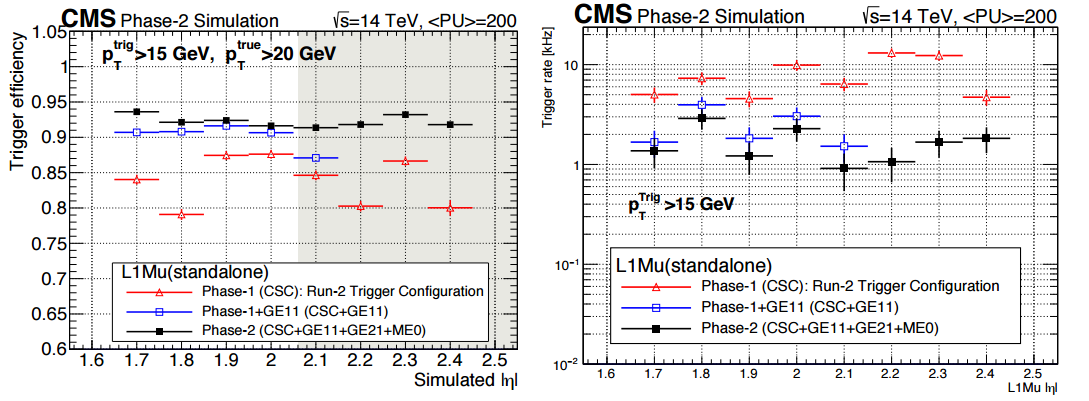
\includegraphics[width=\linewidth]{fig/chapt3/GEM-Trigger.png}
		\caption{\label{fig:GEM-Trigger} Simulated efficiency and rate of the standalone Level-1 muon trigger using tracks reconstructed in CSCs and all GEM stations compared with Phase-I values in the case where only CSCs are used or CSCs+GE1/1. The zones of inefficiency of the CSC subsystem are compensated by the addition of GEMs during Phase-II and the trigger rates is kept from increasing due to the high luminosity.}
	\end{figure}
	
	Adding the GEMs into the forward region of the muon system will allow to strongly enhance the Level-1 Trigger performance by reducing the inefficiency regions and the trigger rate as showed in Figure~\ref{fig:GEM-Trigger}. Moreover, benefiting from the good spatial and angular resolution of the GEMs, the precision into the muon measurement will also be greatly improved by the addition of GEMs as can be seen from the simulation presented in Figure~\ref{fig:GEM-Muon}.
	
	\begin{figure}[H]
		\begin{subfigure}{0.6\linewidth}
			\centering
			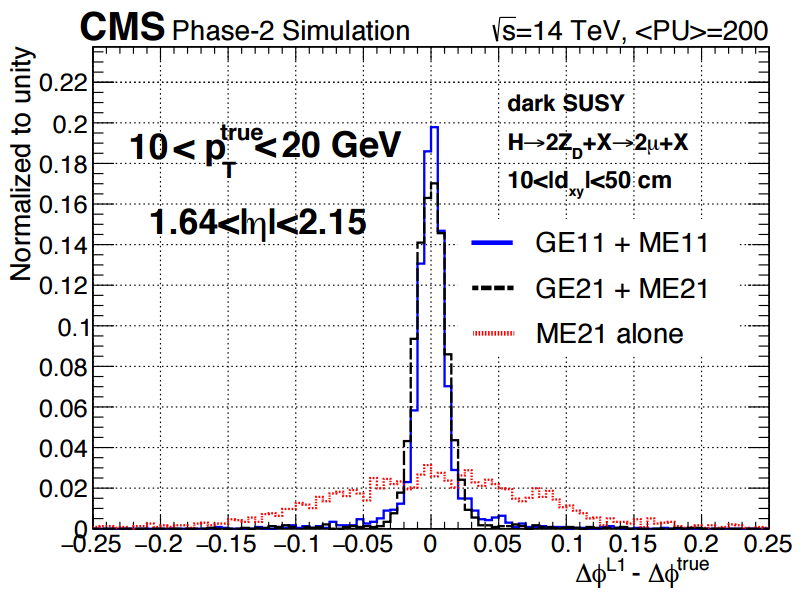
\includegraphics[height=5cm]{fig/chapt3/GEM-muon-direction.png}
			\caption{\label{fig:GEM-Muon:A}}
		\end{subfigure}
		\begin{subfigure}{0.4\linewidth}
			\centering
			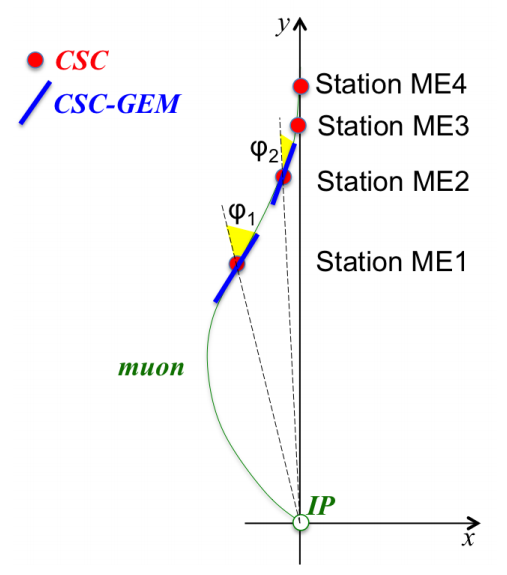
\includegraphics[height=6cm]{fig/chapt3/GEM-Muon-bending.png}
			\caption{\label{fig:GEM-Muon:B}}
		\end{subfigure}
		\caption{\label{fig:GEM-Muon} Figure~\ref{fig:GEM-Muon:A}: Simulated resolution of the muon direction measurement $\Delta\phi$ with Phase-II conditions. In the second endcap station, the resolution is compared in the case of CSCs (ME2/1) alone and CSCs+GEMs (GE2/1+ME2/1) while a similar resolution measurement is given in the case of the first station (GE1/1+ME1/1). Figure~\ref{fig:GEM-Muon:B}: The addition of GEM detectors on stations 1 and 2 (ME0 is considered to contribute to station station 1) as redundant system to CSCs allows to improve the muon momentum improvement through a more accurate measurement of the local bending angles $\phi_1$ and $\phi_2$.}
	\end{figure}

	\begin{figure}[H]
		\centering
		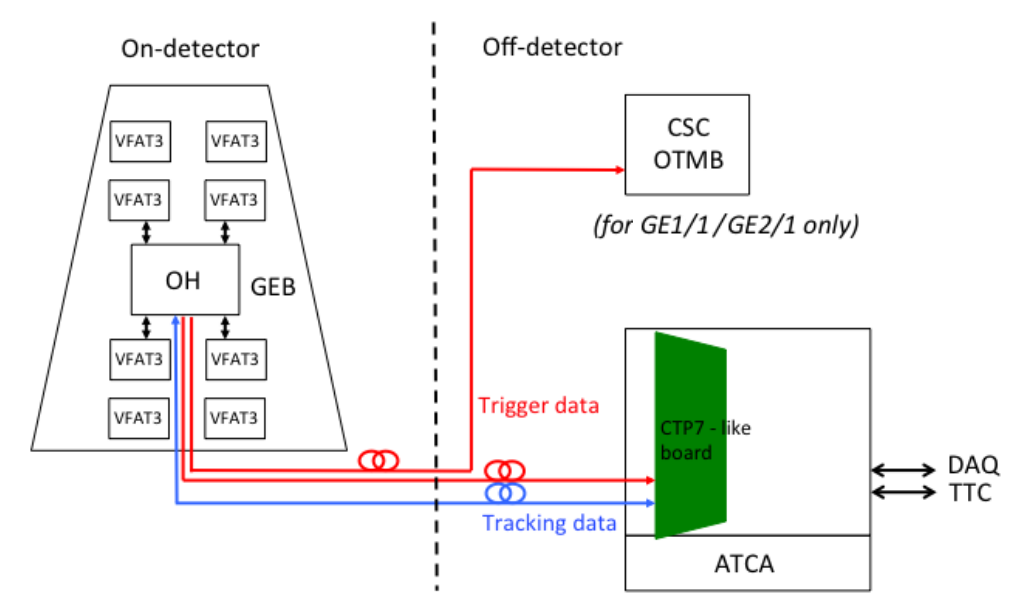
\includegraphics[width=0.8\plotwidth]{fig/chapt3/GEM-electronics.png}
		\caption{\label{fig:GEM-electronics} Schematics of the data communication chain for DAQ of the GEM subsystems. The sending of trigger data via optical links to the CSC OTMBs is only done for GE1/1 and GE2/1 to match the data with ME1/1 and ME2/1.}
	\end{figure}
	
	The read-out of GEMs will use the same technology. The anode planes used as read-out PCBs and referred to as \acf{GEB} host on their outer surface VFAT3 ASICs that connect to a total of 128 strips for a very fine angular granularity. Along the endcap radius, the strips are divided into 8 pseudo-rapidity partitions. In the case of GE1/1 and ME0, each $\eta$-partition consist in 384 read-out strips connected into 3 VFAT3 ASICs and offering a while the large GE2/1 partitions contain twice as many channels. Both GE1/1 and GE2/1 strips have an angular pitch of \SI{474}{\micro m} while this of ME0 is twice larger due to its proximity with the interaction point. The VFAT3 ASICs allow for a latency better than the \SI{12.5}{\micro s} required by CMS Level-1 Trigger and there frequencies goes up to \SI{1}{MHz}. They are connected into the \acf{OH} and this full ensemble (GEB+VAT3+OH) constitute the on-chamber electronics. The OH is then sending the data to the modules constituting the DAQ of the GEM system via optical fibers. These back-end electronics modules are located in the service cavern of CMS and host CMS communication devices, used to have a common clock, and control and links to the \acf{EMTF} system. Moreover, GE1/1 and GE2/1 also have links with the CSC OTMBs as the OH of these 2 subsystems send data into these boards. This communication chain can be seen in Figure~\ref{fig:GEM-electronics}.\\
	
	The detectors that will placed in CMS will have to live through Phase-II without significant performance degradation to ensure an efficient data taking and the possibility to investigate more exotic physics. As the 3 GEM subsystems will be using the same detector technology, the choice was made to certify the GEMs in the worst of the 3 environments, i.e. the ME0 station located right behind the HCAL. According to FLUKA simulation, including all the latest foreseen upgrades into the CMS detector geometry, it was shown that the maximal hit rate expected in ME0 would be of the order of \SI{50}{kHz/cm^2} with contributions of neutrons (\SI{6}{kHz/cm^2}), photons (\SI{35}{kHz/cm^2}), and electrons and positrons (\SI{8}{kHz/cm^2}) resulting in a charge deposition a little lower than \SI{300}{mC/cm^2} after 10 years of HL-LHC~\cite{PHASEIITP}. It is necessary to understand the classical ageing effects on the GEMs but also premature ageing due to contaminants in the gas mixture leading to polymerization on the surface of the GEM foils during operation and the effect of discharges on the detector operations if they have to happen during their lifetime.
	
	\begin{figure}[H]
		\begin{subfigure}{0.5\linewidth}
			\centering
			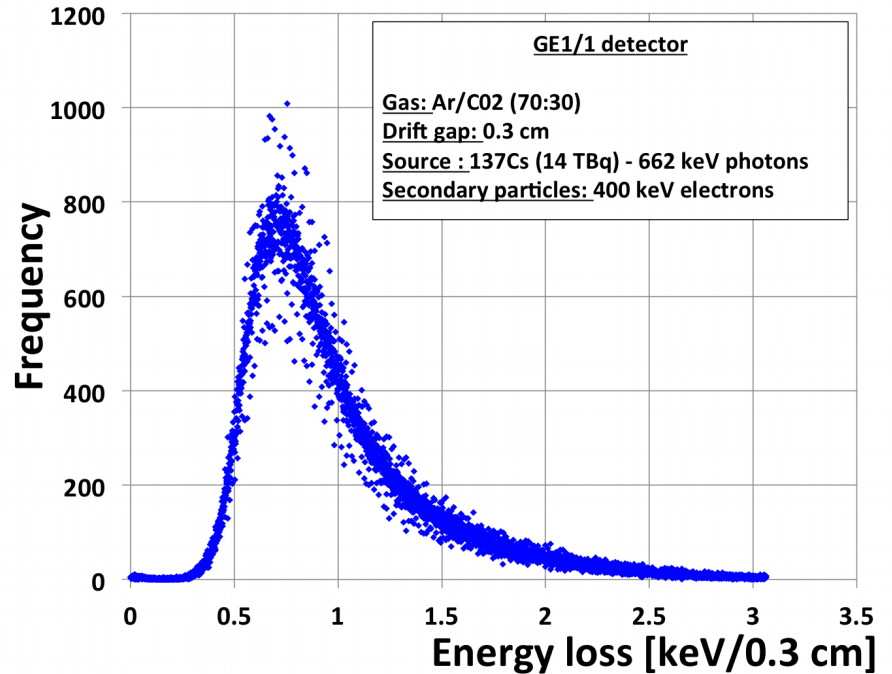
\includegraphics[height=5cm]{fig/chapt3/GEM-GIF-spectrum.png}
			\caption{\label{fig:GEM-longevity:A}}
		\end{subfigure}
		\begin{subfigure}{0.5\linewidth}
			\centering
			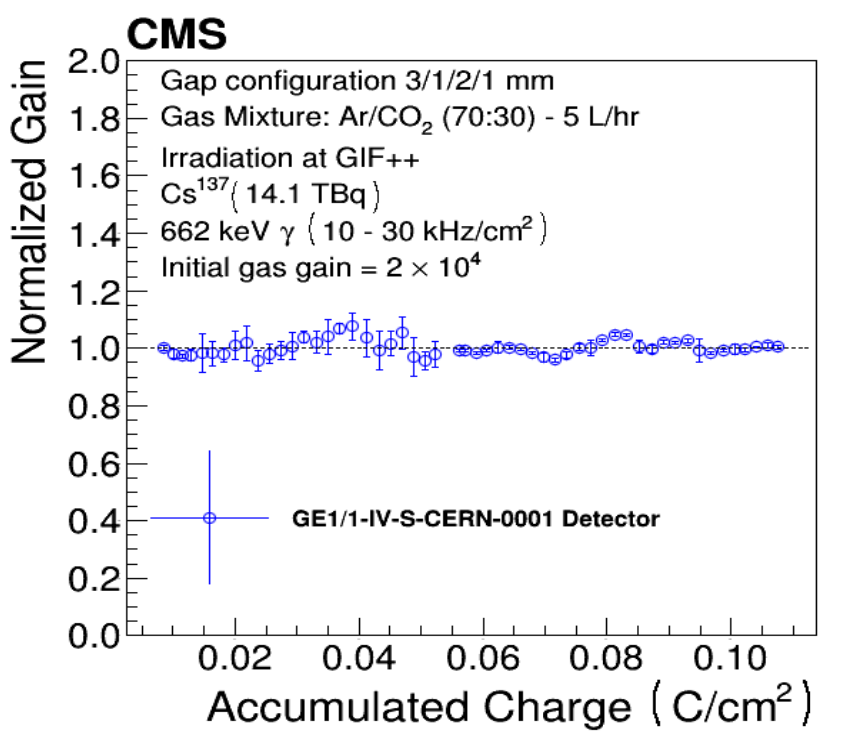
\includegraphics[height=5cm]{fig/chapt3/GEM-GIF-gain-monitor.png}
			\caption{\label{fig:GEM-longevity:B}}
		\end{subfigure}
		\caption{\label{fig:GEM-longevity} Figure~\ref{fig:GEM-longevity:A}: Energy spectrum of GIF++ $^{137}Cs$ source as measured by the GE1/1 detector installed in GIF++. Figure~\ref{fig:GEM-longevity:B}: Evolution of the normalized gain of the GE1/1 detector installed at in GIF++ as a function of the integrated charge per unit area. The first part of the study, up to a charge of \SI{55}{mC/cm^2} had been done in the former \acl{GIF} (GIF) that has now been dismantled following the construction of GIF++. No variation of the normalized gain can be observed after an accumulation of \SI{110}{mC/cm^2}.}
	\end{figure}
	
	To characterize the classical ageing effects, a campaign is being conducted in the \acf{GIF++} of CERN where a GE1/1 detector operated at its nominal gain is placed \SI{50}{cm} from the facility's \SI{14}{TBq} $^{137}Cs$ source which emits gammas at an energy of \SI{662}{keV}. In order to spot any ageing of the detector, the effective gain is kept monitored, as can be seen in Figure~\ref{fig:GEM-longevity:B}, as its variations gives clues about different aspects of the detector such as the geometry of the holes, the electric field configuration or the gas composition. The monitoring of the gamma energy distribution, showed on Figure~\ref{fig:GEM-longevity:A}, can give an idea on the evolution of the performance of the chamber and finally, the evolution of the currents through time also is a good indicator of the appearance of dark current in the detector that would be due to the emission of electrons by thin insulating layers of the detector subjected to a long lasting irradiation known as Malter effect. At the time the \acf{TDR} for the Phase-II upgrade of the muon system was written~\cite{PHASEIITP}, the GEM group had reported a total integrated charge of \SI{110}{mC/cm^2} which, if compared with 10 years of HL-LHC operation, represents a safety factor of 18 for the GE1/1 subsystem and a factor 37 for the GE2/1 subsystem but only 39\% of the total expected ME0 integrated charge. It is estimated that reaching the total integrated charge necessary to certify the detectors for Phase-II operation will take another 2 to 3 years. Nevertheless, the present status of the longevity study shows no degradation of the performance of the detector installed in GIF++ as can be seen through Figure~\ref{fig:GEM-longevity}.
	
	Aside of the classical ageing tests, outgassing of the different materials composing the GEMs have been conducted by placing the different materials to be tested into an outgassing box that consists in a stainless steel cylinder through which the CMS GEM 70/30 gas mixture of $Ar$/$CO_2$ with the possible contaminants is flowed while the detector is exposed to the continuous irradiation of a radioactive source and the heat is raised to enhance the outgassing. From the detector that was placed into this outgassing box, only one component was identified to cause loss of performance due to outgassing. This component was the polyurethane \textit{Cell-Pack} used to coat the internal frame of the GEMs and the polymerization on its surface caused a 20\% decrease of the gas gain. this polyurethane was replaced with a new one for which no outgassing effect causing a loss of performance was reported.
	
	\begin{figure}[H]
		\begin{subfigure}{0.5\linewidth}
			\centering
			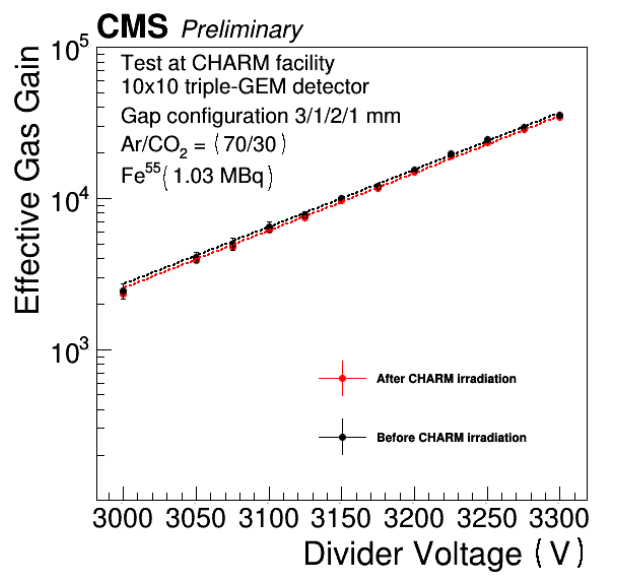
\includegraphics[height=6cm]{fig/chapt3/GEM-CHARM.png}
			\caption{\label{fig:GEM-discharges:A}}
		\end{subfigure}
		\begin{subfigure}{0.5\linewidth}
			\centering
			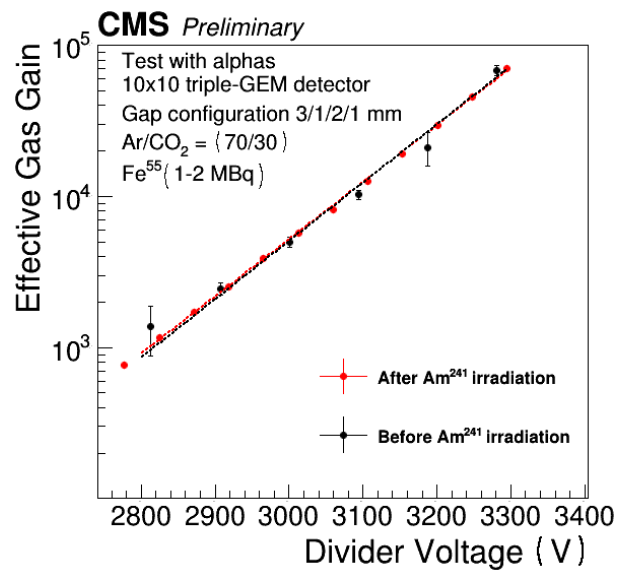
\includegraphics[height=6cm]{fig/chapt3/GEM-alpha.png}
			\caption{\label{fig:GEM-discharges:B}}
		\end{subfigure}
		\caption{\label{fig:GEM-discharges} Figure~\ref{fig:GEM-discharges:A}: Comparison of the gas gain as a function of the divider voltage before and after the irradiation of a triple-GEM by neutrons in CHARM. Figure~\ref{fig:GEM-discharges:B}: Comparison of the gas gain as a function of the divider voltage before and after the irradiation of a triple-GEM by alpha particles.}
	\end{figure}
	
	Finally, even though the triple-GEM technology makes the detectors safe of discharges thanks to its several amplification stages that allow to reach high gas gain using a relatively low electric field applied on the foils and to the distance separating the last foil from the read-out panel that is high enough to prevent discharging from developing all the way to the read-out, and hence, be stopped before it can cause any harm, it is important to have a good understanding of the discharge probability to ensure a safe operation over long periods. In order to further prevent discharges to develop in the detector volume, the GEM foils' power supply have been sectorized and protection resistors have been installed to limit the energy available for the discharge development. To reproduce the high-energy neutron background conditions of CMS, a GE1/1 detector have been placed in the CHARM facility of CERN. This facility allows to irradiate the detectors with a neutron fluence as high as $2.5 \times 10^8$ \si{/cm^2}. The detectors were operated with a slightly higher gain of $3.5 \times 10^4$. It was measured that the discharge probability for a GEM operated under CMS conditions was of $2.85 \times 10^{-9}$ per heavily ionizing particle with a 95\% confidence level that would correspond to 225 discharges per \si{cm^2} in ME0, 17 in GE1/1 and 12 in GE2/1 during the full HL-LHC period. According to Figure~\ref{fig:GEM-discharges:A}, no degradation of the performance was observed after the irradiation at CHARM were 24 discharges per unit area were reported. Nevertheless, another test were the detector was exposed to a \SI{5.5}{MeV} alpha source and were 450 discharges per unit area were reported didn't show any drop of performances either, as can be seen in Figure~\ref{fig:GEM-discharges:B}.
	
	\subsection{Installation schedule}
	\label{chapt3:ssec:schedule}
	
	The previous discussion on the different upgrade projects makes it clear that a lot of work is schedule for CMS to be ready at the end of LS3 for HL-LHC. Conducting all the upgrades of the muon system together with upgrades of the other subsystems like the replacement of the Tracker and of part of the ECAL, will prove to be very difficult as the opening of CMS to access the Barrel will be done by fully opening the endcaps leaving only the first disk to be accessible. Thus, most subsystems have planed early installation over LS2, and the following YETS until LS3 in order to give more space to LS3 schedule.\\
	
	First of all, LS2 will see the installation of GE1/1 detectors, all the on-detector schedule of CSCs and the installation of the necessary services for the improved RPCs to be installed later, such as the HV and LV power supply lines, the gas and cooling lines or signal cables. CSCs will have a huge work to do during LS2 as they will need to extract all of their detectors to refurbish them with upgraded DCFEB and ALCT mezzanine boards. The GE1/1 services were installed during LS1 together with a few demonstrator and only the detectors needs to be integrated into the first endcap disk. The detectors are presently being built and tested at the different assembly site to prepare for a smooth LS2 work.
	
	The work of GEMs will be continued during the following YETS during which is planned the installation of the GE2/1 stations to only leave the ME0 to be installed during LS3. The iRPC program will follow a similar path as the new detectors will be installed during the YETS preceding LS3 in prevision of the fact that the endcap disks will not be accessible during LS3. This way, all the subsystems, but DTs, made great effort on planing their installation and integration within CMS only to have to deal with off-detector issues during the LS3 period, such as the replacement of ODMBs and HV system in the case of CSCs or the upgrade of the RPC Link System. Finallly, during LS3 are schedules the replacement of DT minicrates electronics and the installation and integration of ME0 GEMs together with the HGCAL.
	
\section{Implications of the different upgrades on the Level-1 Trigger. Improvement of physics performance.}
\label{chapt3:sec:L1tP2}

	The upgrades of the different subsystems will have a subsequent impact on the Level-1 Trigger. Indeed, although its main scheme will not be affected, the efficiency of the trigger in efficiency identifying muons and provide the DAQ with good and fast trigger that can cope with HL-LHC instantaneous luminosity is a major improvement. In addition to the upgrade of the muon system in terms of trigger accept rate and latency, the Level-1 Trigger will get extra information in including the Tracker Trigger into its Muon Track Finder logic and combine the L1 Muon Trigger with Tracker and Calorimeter Triggers to generate a Global L1 Trigger with a much better momentum resolution, as showed in Figure~\ref{fig:L1-trigger}.

	\begin{figure}[H]
		\centering
		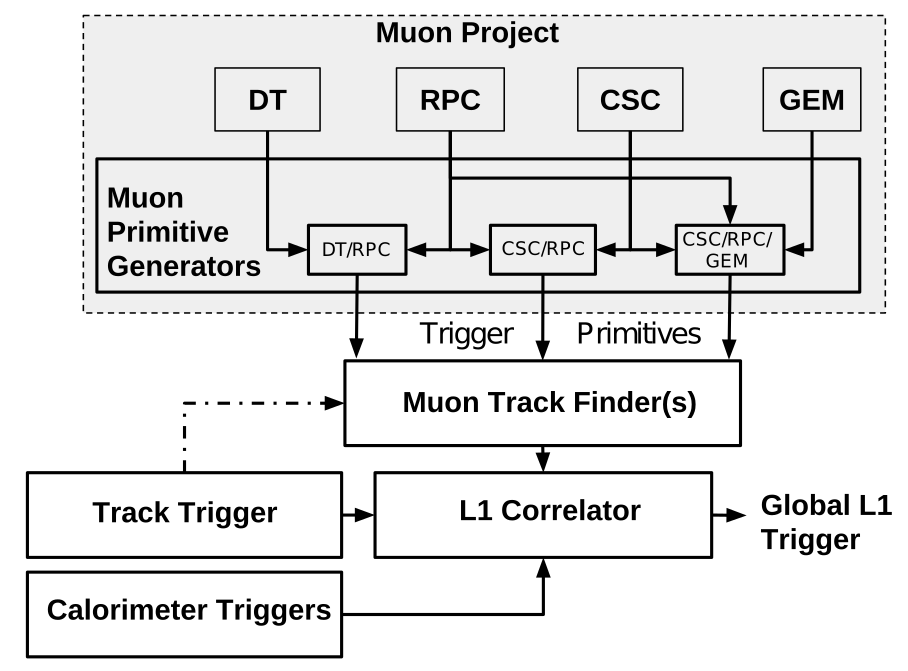
\includegraphics[width=\plotwidth]{fig/chapt3/Phase-II-L1-Trigger.png}
		\caption{\label{fig:L1-trigger} Data flow of the Level-1 Trigger during Phase-II operations.}
	\end{figure}
	
	In terms of muon trigger, 3 regions are considered due to their different track finding logic: the \acf{BMTF}, the \acf{EMTF} for both the barrel and endcap regions, and finally the \acf{OMTF} which concerns the pseudo-rapidity region in which there is a common coverage by both the barrel and endcap muon systems. This region can be seen in Figure~\ref{fig:P2Quadrant} for \psrapr{0.9}{1.2} and requires a specific more complex logic to provide with an efficient reconstruction of the muons due to the different orientation of the detectors and of the more complex magnetic field of this region that needs to be taken into account. The benefits of the upgrade for each of these track finders will be coming from different improvements and will be detailed sector by sector.\\
	
	The main contribution to the improvement of the BMTF is the time resolution improvement of RPC link systems that will allow to take profit of the full \SI{1.5}{ns} resolution of the detectors. From the perspective of RPCs only, this improvement will help reducing the neutron induced background and slightly improve the bunch crossing assignment. The upgrade of DT electronics is also to take into account as the trigger primitive generator will be renewed through the use of TDCs that will send the digitized signals directly to the back-end electronics instead of having an on-detector trigger logic as it will be the case until the end of Phase-I. The front data of both DTs and RPCs will be sent to the same back-end electronics. These upgrades were detailed in section~\ref{chapt3:sec:electronics} and will lead to a more robust operation of the trigger in the barrel region. Indeed, the combination of RPC hits together with DT primitives will bring improvement in the bunch crossing assignment and improve the efficiency of the trigger in between the wheels were the quality of DT primitives is the poorest. Moreover, having a redundant information is important in the case of failure and loos of efficiency of one of either subsystems.

	\begin{figure}[H]
		\centering
		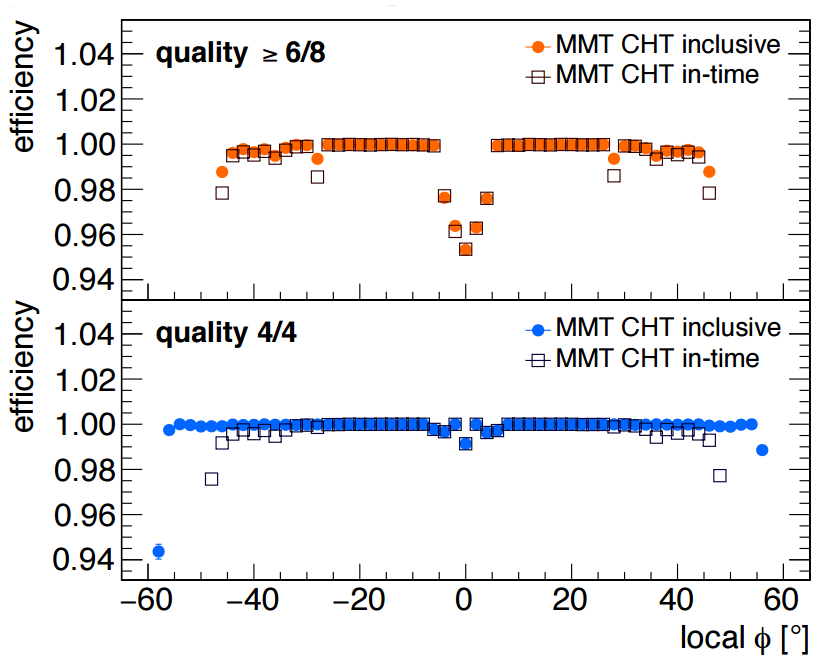
\includegraphics[width=0.7\plotwidth]{fig/chapt3/DT-efficiency-algo.png}
		\caption{\label{fig:DT-P2-eff} Comparison of Phase-II DT trigger primitives algorithmic efficiency for segments obtained with 2 super-layers (quality $\geq$ 6/8) and 1 super-lay only (quality = 4/4). The simulation was done by generating $2 \times 10^6$ muons. The candidate tracks with correct time identification is showed with open symbols.}
	\end{figure}
	
	\begin{figure}[H]
		\begin{subfigure}{0.5\linewidth}
			\centering
			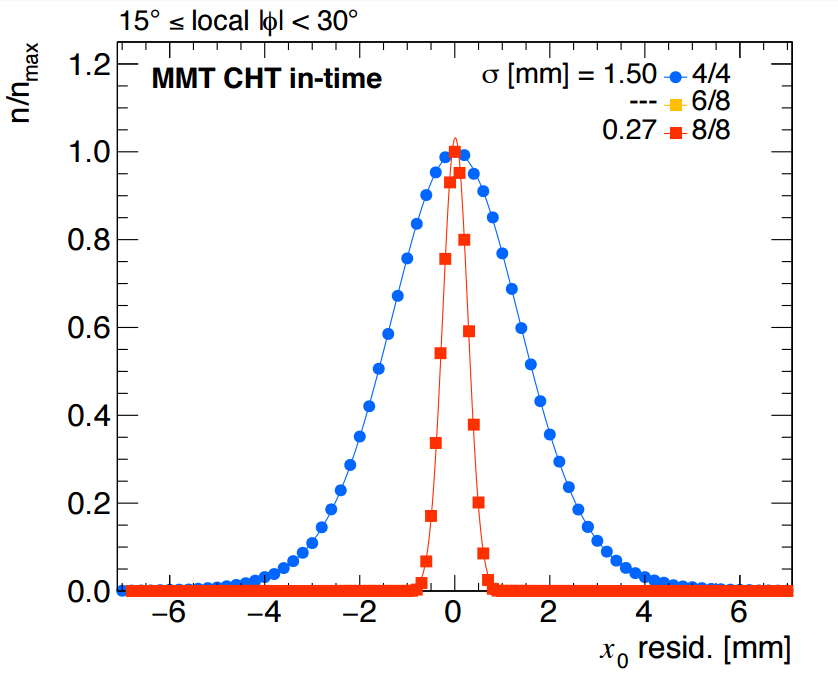
\includegraphics[height=5cm]{fig/chapt3/DT-spatial-res-algo.png}
			\caption{\label{fig:DT-P2-res:A}}
		\end{subfigure}
		\begin{subfigure}{0.5\linewidth}
			\centering
			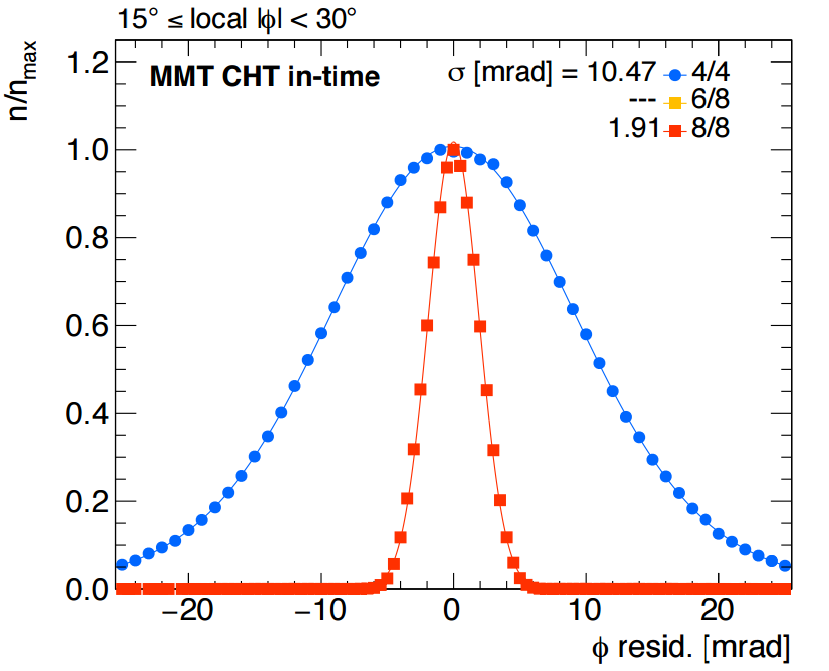
\includegraphics[height=5cm]{fig/chapt3/DT-angular-res-algo.png}
			\caption{\label{fig:DT-P2-res:B}}
		\end{subfigure}
		\caption{\label{fig:DT-P2-res} Simulated spatial (\ref{fig:DT-P2-res:A}) and angular (\ref{fig:DT-P2-res:B}) resolution of the algorithm using 8 aligned hits in both super-layers (quality = 8/8) and 4 aligned hits in only one super-layer (quality = 4/4). The contribution of intermediate quality tracks (6 aligned hits) is negligible in the angular range shown. \textbf{[Be careful to update this caption as it uses a text to close to the published one.]}}
	\end{figure}
	
	The loss of single hit efficiency of DTs due to ageing will also force the DT to change the algorithm use to identify tracks. So far, the identification was only performed at the level of a single DT super-layer, which is composed of 4 single DT layers. In the perspective the single efficiency drops, this will require to be upgraded to try to combine the data of more than a single super-layer to keep a high muon track identification efficiency. In addition to this change in trigger primitive candidate quality, new algorithms with higher efficiency are being developed. According to Figure~\ref{fig:DT-P2-eff}, the efficiency of the new algorithm, both in the cases using 1 or 2 super-layers, is higher than with the current system~\cite{CMS2013}. Moreover, the overall efficiency of an algorithm requesting at least a muon detected in 6 DT layers out of the 8 composing the 2 super-layers of a DT module would stay comparable to the 4 DT layers out of 4 algorithm within the local bending angle range. On the other hand, despite the slight loss of efficiency in the low angle range, the algorithm using more DT layers achieves both higher spatial and angular resolution according to Figure~\ref{fig:DT-P2-res}.\\
	
	With new detectors to cover the very forward region and the upgrade of RPC Link System, the EMTF will be greatly improved. The current EMTF already use more sophisticated algorithms by combining together RPC hits and CSC primitives and will also benefit from the improved time resolution of the RPC system. The GEMs, in stations 1 and 2, and the iRPCs, in stations 3 and 4, will be added into the EMTF algorithm. Both these contributions will help increasing the efficiency of the L1 trigger in the endcap region in one hand, and help lowering the L1 trigger rate in the other hand, especially in the most forward region. The improvement of the efficiency will come both from the better time resolution of RPC link boards and from the addition of more hits along the muon tracks and also a contribution from the GEMs to the lever arm of each track thanks to there high angular resolution.
	
	The rate will be partly reduced in the forward region thanks to the better spatial resolution of iRPCs, with respect to the current RPC system, that will reduce the ambiguity brought by multiple local charged tracks in CSCs, as explained through Figure~\ref{fig:LCT-ambiguity}. Indeed, as the rates will increase, the probability to record more than a single local charged track will greatly increase. This is due to the fact that the trigger algorithm uses information from 3 consecutive bunch crossings to find muon tracks. It is estimated that with iRPCs operated at 95\% efficiency the resolution of ambiguous events would be of the order of 99.7\%.
	
	\begin{figure}[H]
		\begin{subfigure}{0.5\linewidth}
			\centering
			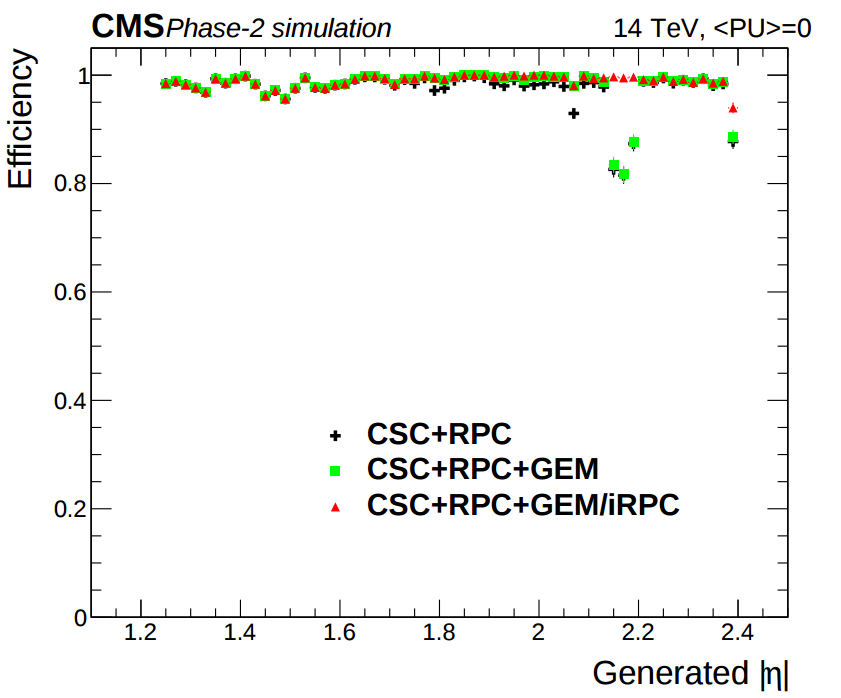
\includegraphics[height=5cm]{fig/chapt3/EMTF-eff-2of4.png}
			\caption{\label{fig:EMTF-eff:A}}
		\end{subfigure}
		\begin{subfigure}{0.5\linewidth}
			\centering
			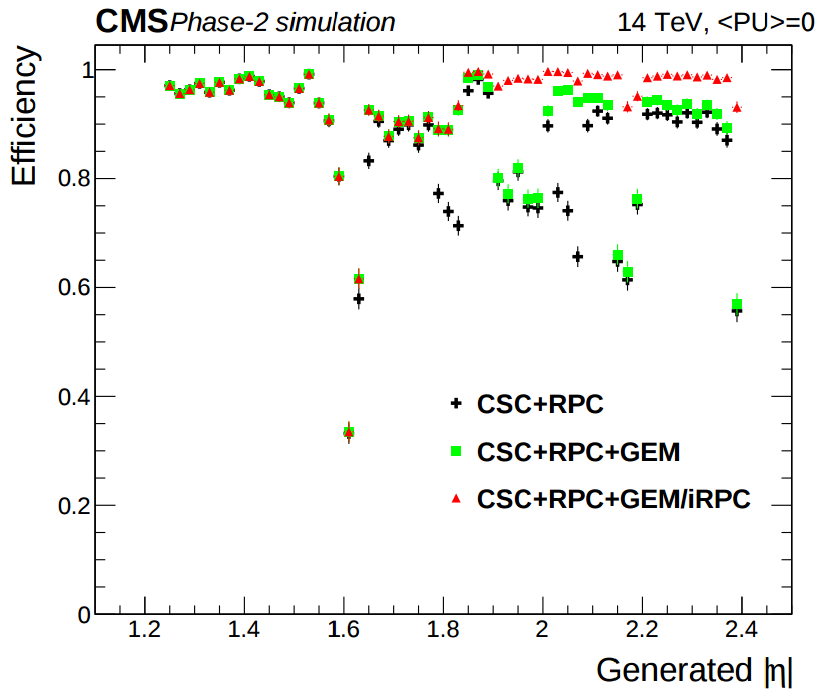
\includegraphics[height=5cm]{fig/chapt3/EMTF-eff-4of4.png}
			\caption{\label{fig:EMTF-eff:B}}
		\end{subfigure}
		\caption{\label{fig:EMTF-eff} Efficiency of the L1 trigger in the endcap region after Phase-II upgrade in the case CSC/GEM/RPC hits are requested in at least 2 stations out of four (\ref{fig:EMTF-eff:A}) and in all four stations (\ref{fig:EMTF-eff:B}).}
	\end{figure}

	\begin{figure}[H]
		\centering
		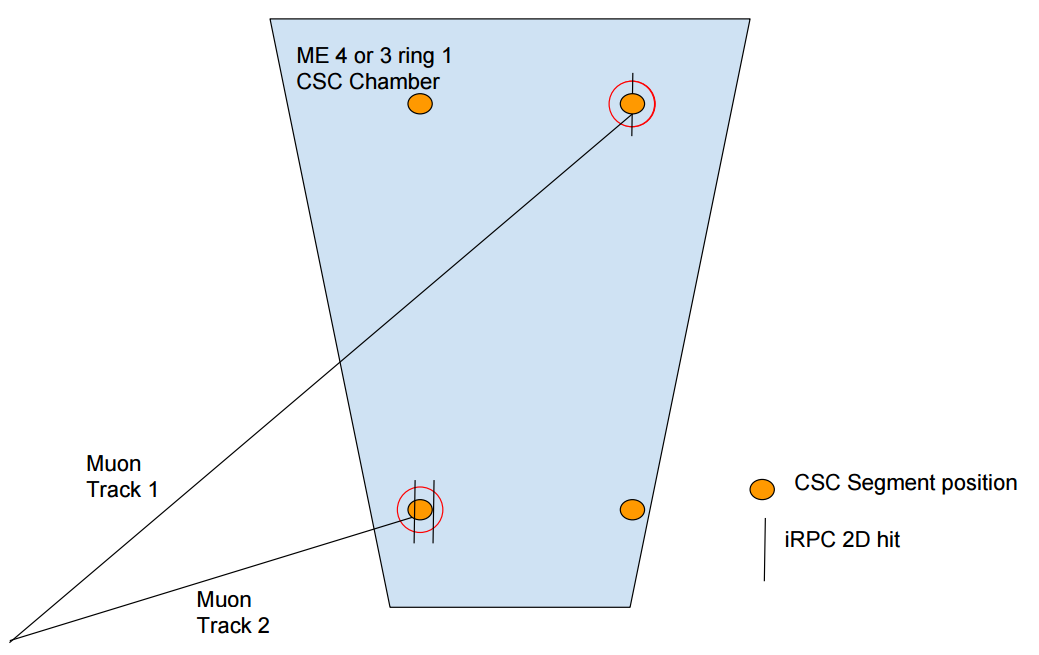
\includegraphics[width=0.9\plotwidth]{fig/chapt3/CSC-LCT-ambiguity.png}
		\caption{\label{fig:LCT-ambiguity} Resolution of the LCT ambiguous events thanks to the combination of CSC and iRPC readout data. Using CSCs only, 2 pairs of hits are possible.}
	\end{figure}
	
	The addition of GEMs will improve greatly the measured muon momentum resolution by improving the global resolution of the direction of muon tracks, as can be seen in Figure~\ref{fig:CSC-GEM-res}, which will contribute to lowering the trigger rate and increase the efficiency, as can be seen from Figure~\ref{fig:CSC-GEM-perf} that focuses especially in the most challenging pseudo-rapidity region. Data from both CSCs and GEMs are combined into the OTMB to build on each station, GEM/CSC primitives matching space and time information from both subsystems.
	
	Finally, the development of a track finder specific to the overlap region was already achieved during the Phase-I upgrade of the L1-Trigger~\cite{L1UPGRADE2016}. Nevertheless, the improvements of DT spatial resolution and RPC timing will be carried and implemented into the OMTF.
	
	\begin{figure}[H]
		\begin{subfigure}{0.5\linewidth}
			\centering
			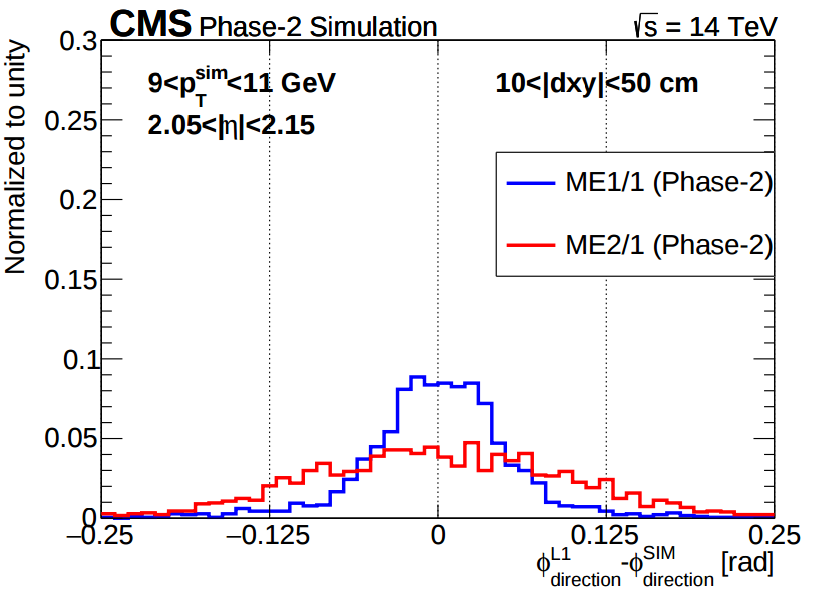
\includegraphics[height=5cm]{fig/chapt3/CSC-angular-res.png}
			\caption{\label{fig:CSC-GEM-res:A}}
		\end{subfigure}
		\begin{subfigure}{0.5\linewidth}
			\centering
			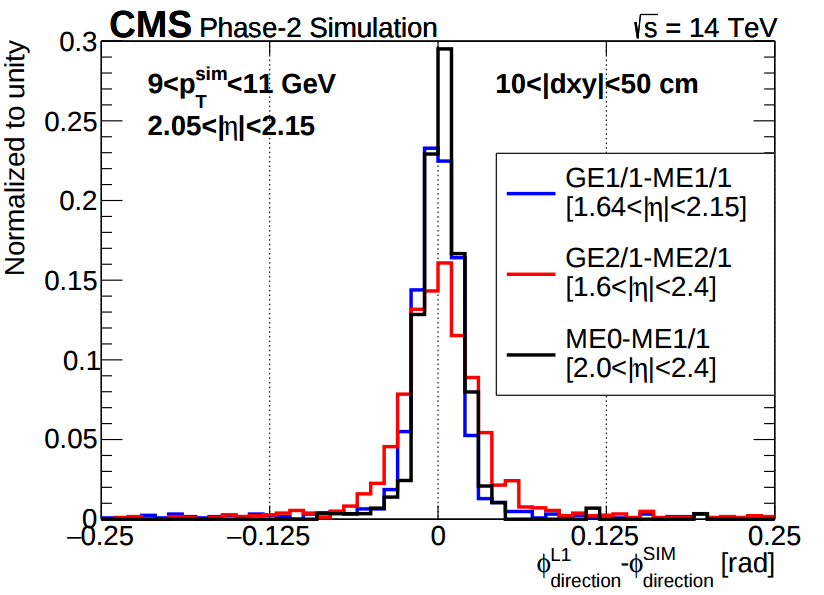
\includegraphics[height=5cm]{fig/chapt3/GEM-angular-res.png}
			\caption{\label{fig:CSC-GEM-res:B}}
		\end{subfigure}
		\caption{\label{fig:CSC-GEM-res} The angular resolution on reconstructed muon tracks in the GEM overlap region \psrapr{2.0}{2.15} is compared for Phase-II conditions in the case CSC are alone (Figure~\ref{fig:CSC-GEM-res:A}) and in the case the GEMs' data, including ME0, is combined to which of CSCs (Figure~\ref{fig:CSC-GEM-res:B}).}
	\end{figure}
	
	\begin{figure}[H]
		\begin{subfigure}{0.5\linewidth}
			\centering
			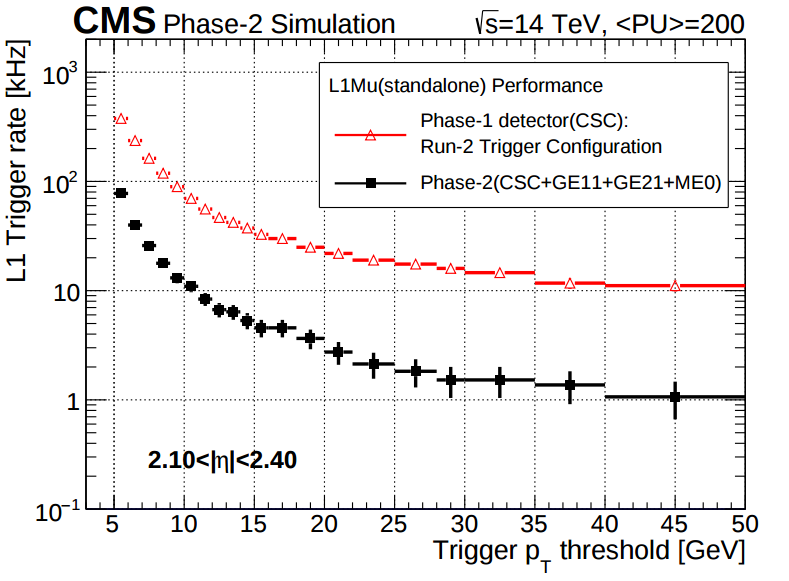
\includegraphics[height=5cm]{fig/chapt3/GEM-trigger-rate.png}
			\caption{\label{fig:CSC-GEM-perf:A}}
		\end{subfigure}
		\begin{subfigure}{0.5\linewidth}
			\centering
			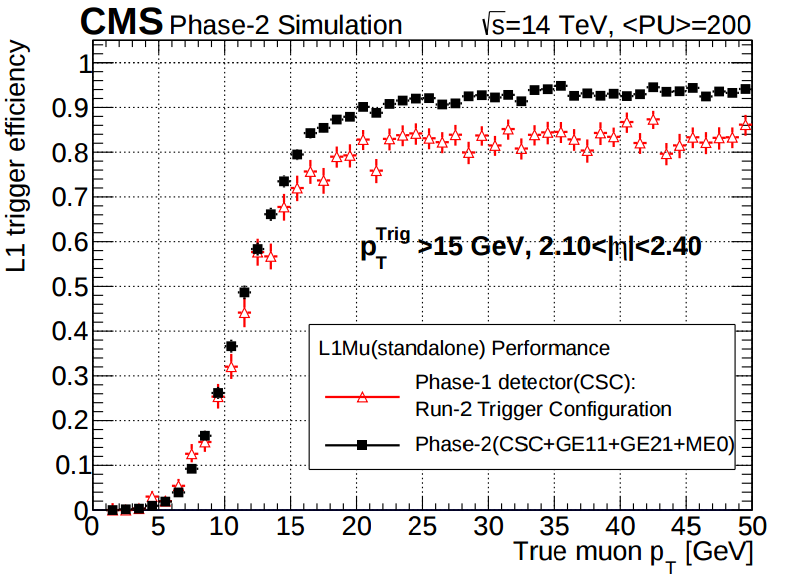
\includegraphics[height=5cm]{fig/chapt3/GEM-trigger-eff.png}
			\caption{\label{fig:CSC-GEM-perf:B}}
		\end{subfigure}
		\caption{\label{fig:CSC-GEM-perf} Comparison of L1 trigger performances for prompt muons with and without the addition of GEMs in the region \psrapr{2.1}{2.4} at Phase-II conditions. GEMs would allow a reduction of the trigger accept rate by an order of magnitude (Figure~\ref{fig:CSC-GEM-perf:A}) while increasing the trigger efficiency (Figure~\ref{fig:CSC-GEM-perf:B}).}
	\end{figure}

\section{Ecofriendly gas studies}
\label{chapt3:sec:EcoGas}

	Future strict restrictions in the use of certain gases. The European Commission adopted a new "F-gas regulation" in 2014~\cite{EUFGAS2014} with the goal to strongly control and reduce the use of fluorinated gases with high \acf{GWP}. Using $CF_4$, $C_2H_2F_4$ and $SF_6$, both CSC and RPC subsystems will need to address this problem by finding new gas mixture for the operation of their detectors. Finding a replacement for these gas component that were used for very specific reasons will be a great challenge. Indeed, CSCs use $CF_4$ in order to enhance the longevity of the detectors, increase the drift velocity of electrons and quench photons with a non-flammable gas mixture. RPCs use a mixture mainly composed of $C_2H_2F_4$, that features a high effective Townsend coefficient and the great average fast charge allowing for operations with a high threshold, and contains a small fraction of of $SF_6$ that is used for its electronegative properties that prevents the development of delta-rays in the gas volume that might trigger multiple ionization and avalanches.
	
	\begin{table}[H]
		\centering
		\begin{tabular}{l c c}
			\hline
			 & CSC & RPC\\
			\hline
			Greenhouse gases used & $CF_4$ & $C_2H_2F_4$ and $SF_6$ \\
			Greenhouse gases fraction in the gas mixture & 10\% & 95.2\% and 0.3\% \\
			Global Warming Potential (relative to $CO_2$) & 6500 & 1300 and 23900 \\
			Gas mixture re-circulation & Yes, 90\% & Yes, 85\% \\
			Gas mixture replenishing rate (\si{l/hr}) & 700 & 1100 \\
			F-gas recuperation & Yes, $\approx$40\% & No \\
			F-gas venting rate (\si{l/hr}) & 42 & 1047 and 3.3 \\
			$CO_2$-equivalent rate (\si{m^3/h}) & 273 & 1440 \\
			Relative impact (entire muon system = 100\%) & 16\% & 84\% \\
			\hline
		\end{tabular}
		\caption{\label{tab:F-GAS-CMS} Details of the greenhouse fluorinated gases used in CMS and of their GWP~\cite{PHASEIITP}.}
	\end{table}
	
	Nevertheless, all these gases have a very high GWP, as reported in Table~\ref{tab:F-GAS-CMS}, and only few options are left. The subsystems need to work on strongly decrease the loss of these gases due to leaks in the gas system or completely change their gas mixture for more ecofriendly ones. Reducing the gas leaks on the current system will require installation of a F-gas recuperation system on RPCs side and an upgrade of CSCs existing one in addition to the repair of existing leaks. It is expected that the total leak rate would represent only 1.6\% of the current levels~\cite{PHASEIITP}. In the case the F-gas were to be banned, it would be necessary to have replacement mixtures to operate CMS. CSC is presently investigating replacement for $CF_4$ such as $CF_3I$, $C_4F_6$, $IC_3F_6$, $C_3F_8$ or $CHF_3$ while RPCs, in collaboration with the ATLAS RPC group which uses the same gas mixture and, hence, faces similar restrictions, have identified $CF_3I$ (GWP $leq$ 1) and $C_3H_2F_4$ (GWP $\approx$ 6), referred to as HFO-1234ze, as potential candidates with mixtures containing $CO_2$ but more R\&D needs to be conducted for both subsystems before concluding on the best alternative. The status of RPC studies are presented in Figure~\ref{fig:RPC-eco} in which the performance (efficiency and streamer probability) of an RPC operated with alternative gas mixtures is compared to the present CMS RPC mixture.
	
	\begin{figure}[H]
		\hspace*{-0.1\linewidth}
		\begin{subfigure}{0.6\linewidth}
			\centering
			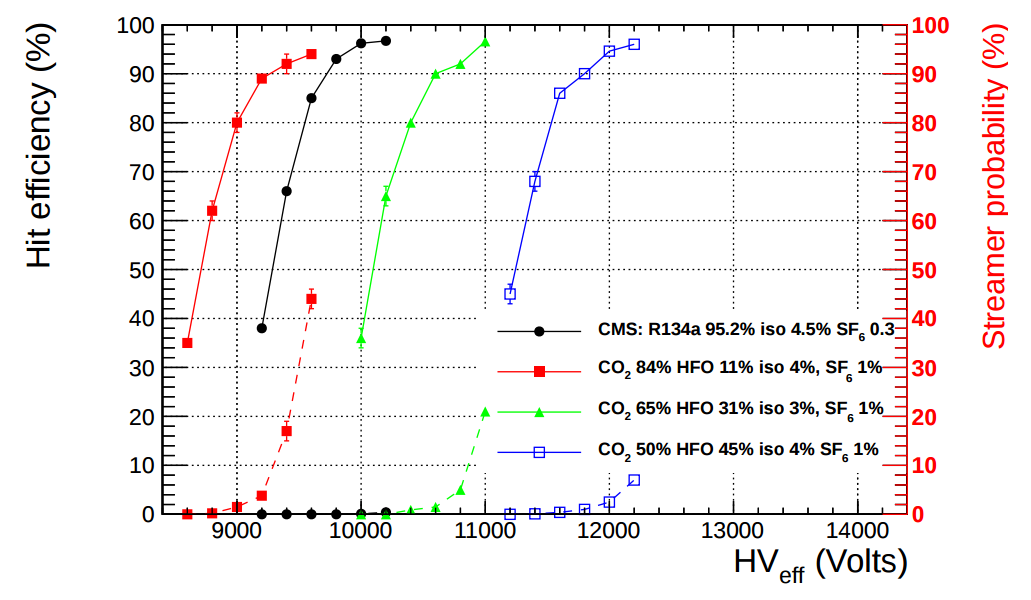
\includegraphics[height=5cm]{fig/chapt3/HFO-mixtures.png}
			\caption{\label{fig:RPC-eco:A}}
		\end{subfigure}
		\begin{subfigure}{0.6\linewidth}
			\centering
			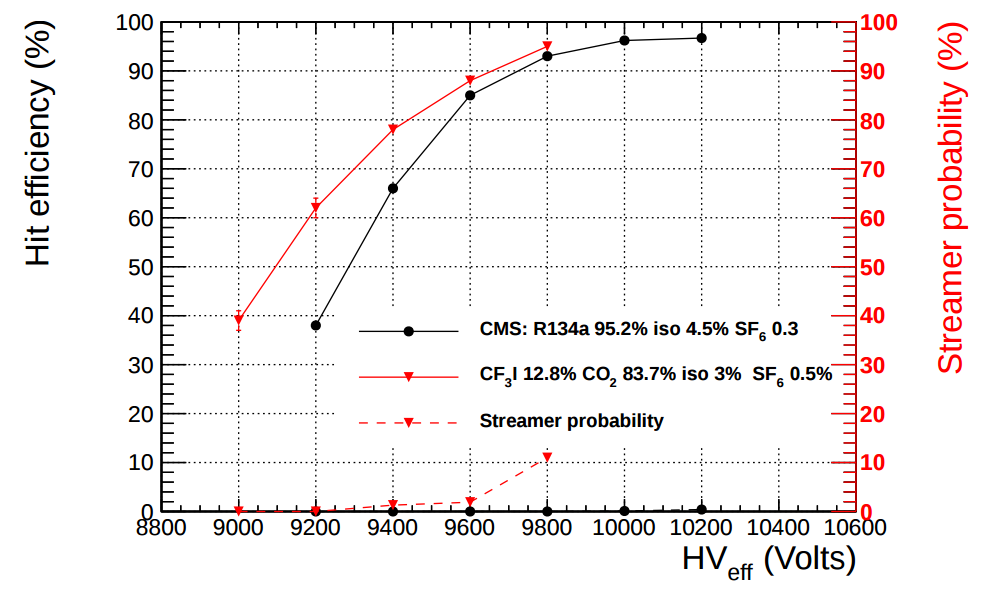
\includegraphics[height=5cm]{fig/chapt3/CF3I-mixture.png}
			\caption{\label{fig:RPC-eco:B}}
		\end{subfigure}
		\caption{\label{fig:RPC-eco} The efficiency (solid lines) and streamer probability (dashed lines) of $HFO$/$CO_2$ (Figure~\ref{fig:RPC-eco:A}) and $CF_3I$/$CO_2$ (Figure~\ref{fig:RPC-eco:B}) based gas mixtures as a function of the effective high-voltage are compared with the present CMS RPC gas mixture represented in black. The streamer probability is defined as the proportion of events with a deposited charge greater than \SI{20}{pC}.}
	\end{figure}

	\subsection{Status of the studies and potential candidates}
	\label{chapt3:ssec:GasStatus}

	\subsection{Implications in case of no suitable ecofriendly mixture}
	\label{chapt3:ssec:GasConsequences}

\clearpage{\pagestyle{empty}\cleardoublepage}
\graphicspath{{chapt_dutch/}{intro/}{chapt2/}{chapt3/}{chapt4/}{chapt5/}{chapt6/}{chapt7/}}

% Header
\renewcommand\evenpagerightmark{{\scshape\small Chapter 4}}
\renewcommand\oddpageleftmark{{\scshape\small Resistive Plate Chambers}}

\renewcommand{\bibname}{References}

\hyphenation{}

\chapter[Resistive Plate Chambers]%
{Resistive Plate Chambers}
\label{chapt:4}

\section{Principle}
\label{sec:principle}

\section{Rate capability of Resistive Plate Chambers}
\label{sec:RateCapa}

\section{High time resolution}
\label{sec:TimeRes}

\section{Resistive Plate Chambers at CMS}
\label{sec:CMS-RPC}

    \subsection{Pulse processing of CMS RPCs}
    \label{ssec:PulseProc}
	
		Signals induced by cosmic particle in the RPC strips are shaped by standard CMS RPC \acf{FEE} following the scheme of Figure~\ref{fig:DAQ}. On a first stage, analogic signals are amplified and then sent to the \acf{CFD} described in Figure~\ref{fig:CFD}. At the end of the chain, \SI{100}{ns} long pulses are sent in the LVDS output. These output signal are sent on one side to a V1190A \acf{TDC} module from CAEN and on the other to an OR module to count the number of detected signals. Trigger and hit coïncidences are monitored using scalers. The TDC is used to store the data into ROOT files. These files are thus analysed to understand the detectors performance.

			\begin{figure}[!h]
			\begin{subfigure}{\linewidth}
				\centering
				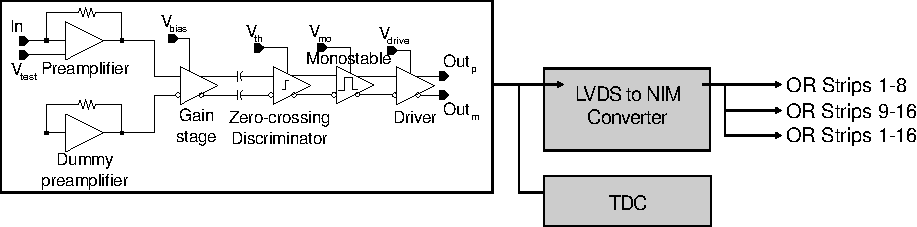
\includegraphics[width = \plotwidth]{fig/chapt5/pulse-processing.pdf}\\
				\caption{\label{fig:DAQ:A}}
			\end{subfigure}
			\begin{subfigure}{\linewidth}
				\centering
				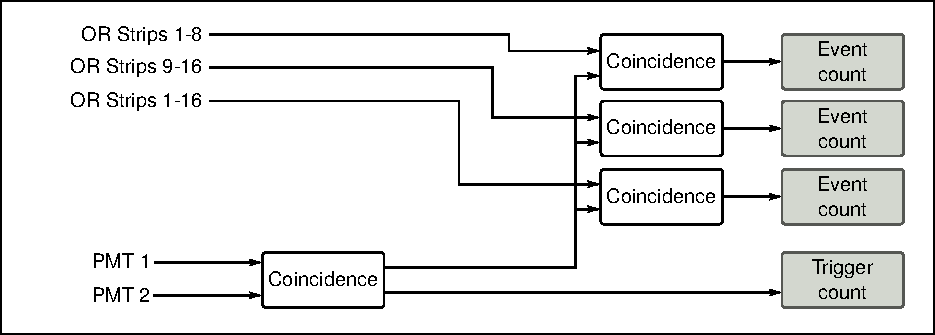
\includegraphics[width = \plotwidth]{fig/chapt5/pulse-processing-2.pdf}
				\caption{\label{fig:DAQ:B}}
			\end{subfigure}
			\caption{\label{fig:DAQ} Signals from the RPC strips are shaped by the FEE described on Figure ~\ref{fig:DAQ:A}. Output LVDS signals are then read-out by a TDC module connected to a computer or converted into NIM and sent to scalers. Figure~\ref{fig:DAQ:B} describes how these converted signals are put in coincidence with the trigger.}
		\end{figure}
		
		\begin{figure}[!h]
			\begin{subfigure}{\linewidth}
				\centering
				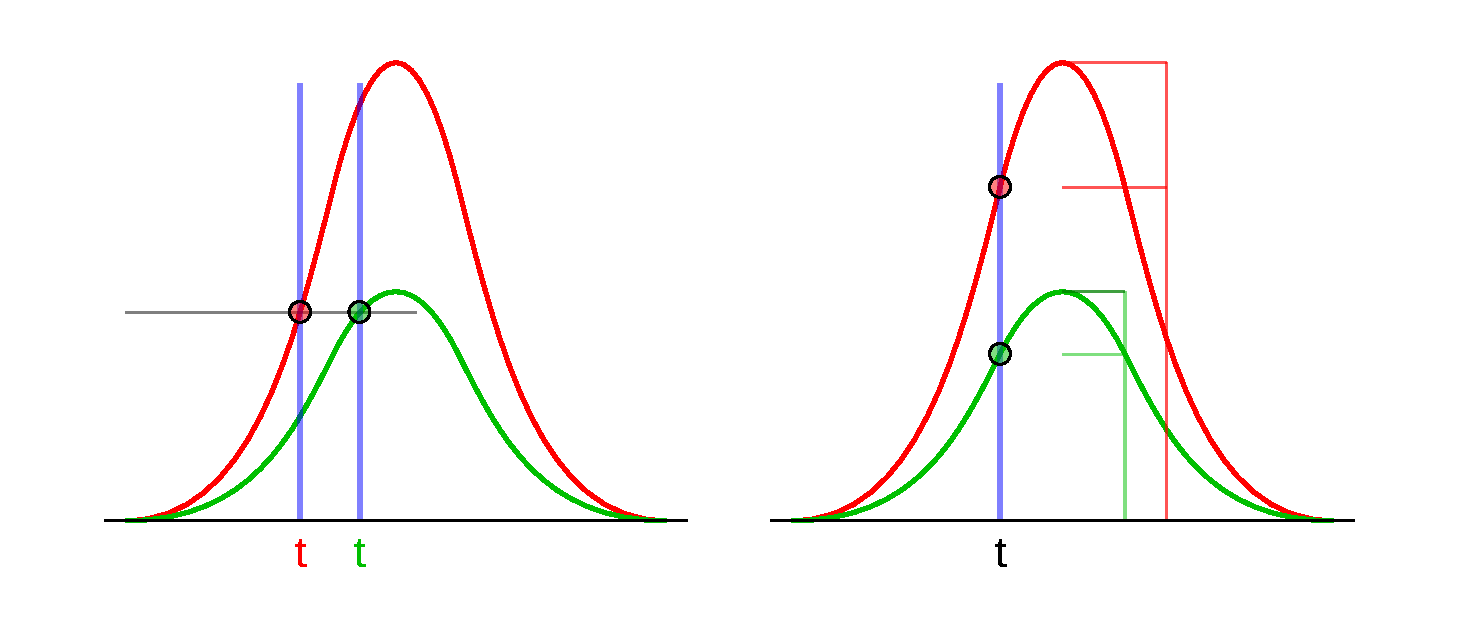
\includegraphics[width = \plotwidth]{fig/chapt5/CFD_1.pdf}\\
				\caption{\label{fig:CFD:A}}
			\end{subfigure}
			\begin{subfigure}{\linewidth}
			    \centering
				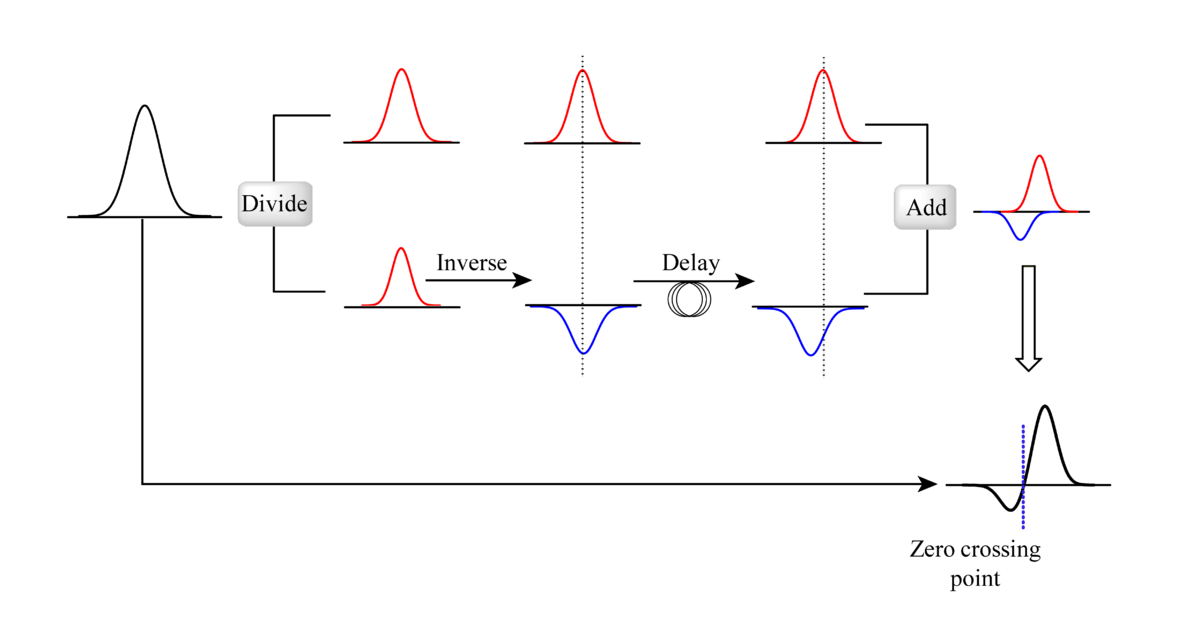
\includegraphics[width = 1.2\plotwidth]{fig/chapt5/CFD_2.png}
				\caption{\label{fig:CFD:B}}
			\end{subfigure}
			\caption{\label{fig:CFD} Description of the principle of a CFD. A comparison of threshold triggering (left) and constant franction triggering (right) is shown in Figure~\ref{fig:CFD:A}. Constant franction triggering is obtained thanks to zero-crossing technique as explained in Figure~\ref{fig:CFD:B}. The signal arriving at the input of the CFD is split into three components. A first one is delayed and connected to the inverting input of a first comparator. A second component is connected to the noninverting input of this first comparator. A third component is connected to the noninverting input of another comparator along with a threshold value connected to the inverting input. Finally, the output of both comparators is fed through an AND gate.}
		\end{figure}

\clearpage{\pagestyle{empty}\cleardoublepage}

% Header
\renewcommand\evenpagerightmark{{\scshape\small Chapter 5}}
\renewcommand\oddpageleftmark{{\scshape\small Longevity studies and Consolidation of the present CMS RPC subsystem}}

\renewcommand{\bibname}{References}

\hyphenation{}

\chapter[Longevity studies and Consolidation of the present CMS RPC subsystem]{Longevity studies and Consolidation of the present CMS RPC subsystem}
\label{chapt5}
    
	The RPC system, located in both barrel and endcap regions, provides a fast, independent muon trigger with a looser \pT threshold over a large portion of the pseudo-rapidity range (\psrapl{1.6}). During HL-LHC operations the expected conditions in terms of background and pile-up will make the identification and correct \pT assignment a challenge for the muon system. The goal of RPC upgrade is to provide additional hits to the Muon System with more precise timing. All this information will be elaborated by the Trigger System in a global way enhancing the performance of the trigger in terms of efficiency and rate control. The RPC Upgrade is based on two projects: an improved Link Board System and the extension of the RPC coverage up to \psrape{2.4}.

	The Link Board System is responsible for the processing, the synchronization and the zero-suppression the signals coming from the RPC FEBs. The Link Board components have been produced between 2006 and 2007 and will be subjected to ageing and failure on a long term scale. An upgraded Link Board System will overcome the ageing problems and will allow for a more precise timing information to the RPC hits from 25 to \SI{1.5}{ns}.\\
	In order to develop an improved RPC that fulfills CMS requirements, an extensive R\&D program is being conducted. The benefits of adding two new RPC layers in the innermost ring of stations 3 and 4 will be mainly observed in the neutron-induced background reduction and efficiency improvement for both trigger and offline reconstruction.

	The coverage of the RPC System up to higher pseudo-rapidity \psrape{2.1} was part of the original CMS TDR. Nevertheless, the expected background rates being higher than the certified rate capability of the present CMS RPCs in that region and the budget being limited, RPCs were restricted to a shorter range. Even though the iRPC technology that will equip the extension of the Muon System will be different than the current CMS RPC technology, it is necessary to certify the rate capability and longevity of the existing detectors as the radiation level will increase together with the increase of instantaneous luminosity of the LHC. For this purpose, spare RPC detectors built but not installed in CMS have been installed in different irradiation facilities, first of all, to certify the detectors to the new levels of irradiation they will be subjected to and, finally, to study their ageing and certify their good operation throughout the HL-LHC program.

\section{Testing detectors under extreme conditions}
\label{chapt5:sec:extreme}

	The upgrade from LHC to HL-LHC will increase the peak luminosity from \Ord{34} \siflux to reach \Sci{5}{34} \siflux, increasing in the same way the total expected background to which the RPC System will be subjected to. Mainly composed of low energy gammas, neutrons, and electrons and positrons from $p$-$p$ collisions, but also of low momentum primary and secondary muons, punch-through hadrons from calorimeters, and particles produced in the interaction of the beams with collimators, the background will mostly affect the regions of CMS that are the closest to the beam line, i.e. the RPC detectors located in the endcaps.
    
	\begin{figure}[H]
		\begin{subfigure}{0.5\linewidth}
			\centering
			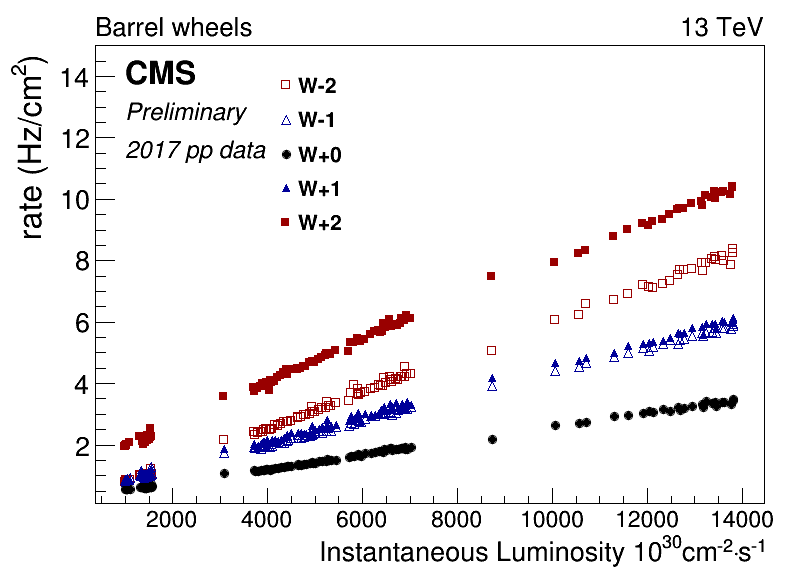
\includegraphics[height=5cm]{fig/chapt5/Rate-vs-Lumi-Barrel.png}
			\caption{\label{fig:Rate-I-vs-Lumi:A}}
		\end{subfigure}
		\begin{subfigure}{0.5\linewidth}
			\centering
			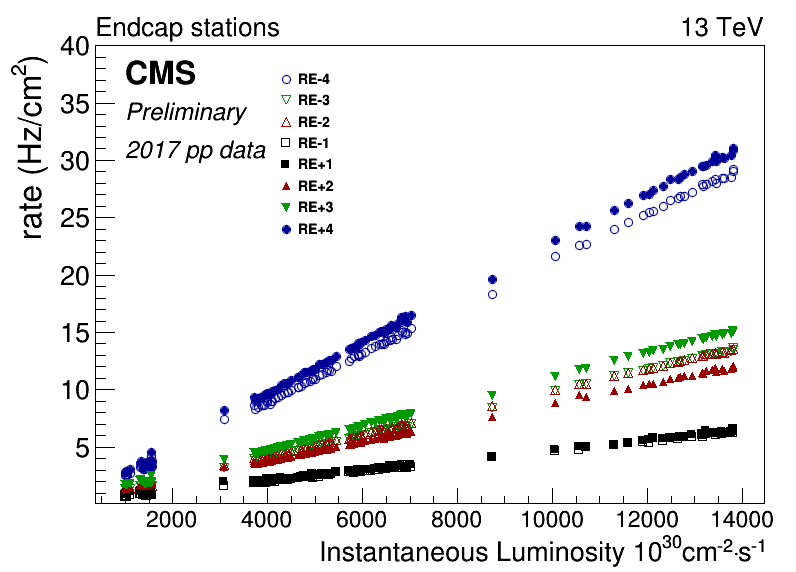
\includegraphics[height=5cm]{fig/chapt5/Rate-vs-Lumi-Endcap.png}
			\caption{\label{fig:Rate-I-vs-Lumi:B}}
		\end{subfigure}
		\begin{subfigure}{0.5\linewidth}
			\centering
			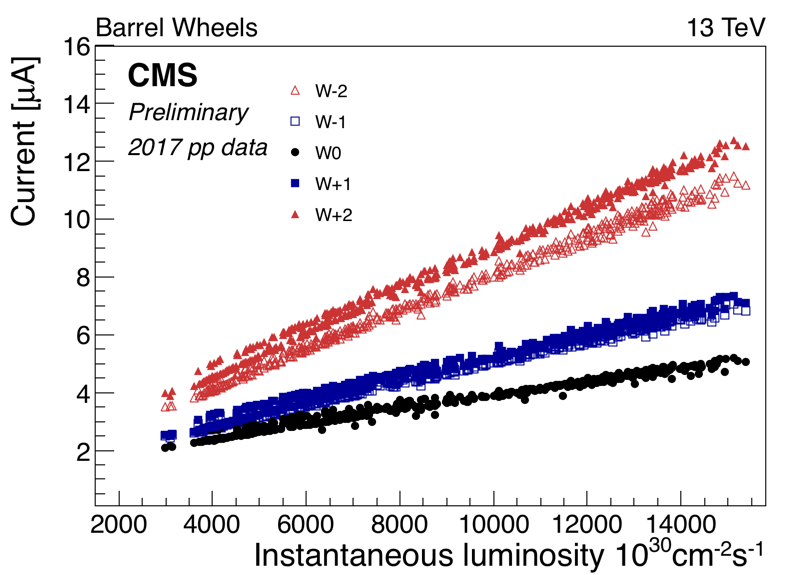
\includegraphics[height=5cm]{fig/chapt5/Current-vs-Lumi-Barrel.png}
			\caption{\label{fig:Rate-I-vs-Lumi:C}}
		\end{subfigure}
		\begin{subfigure}{0.5\linewidth}
			\centering
			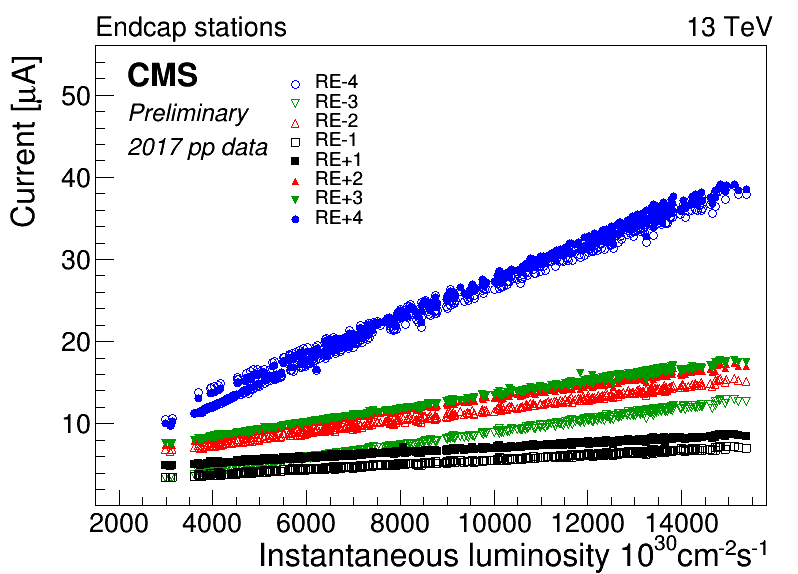
\includegraphics[height=5cm]{fig/chapt5/Current-vs-Lumi-Endcap.png}
			\caption{\label{fig:Rate-I-vs-Lumi:D}}
		\end{subfigure}
		\caption{\label{fig:Rate-I-vs-Lumi} Mean RPC Barrel (left column) and Endcap (right column) rate (top row) and current (bottom row) as a function of the instantaneous luminosity as measured in 2017 $p$-$p$ collision data.}
	\end{figure}

	Data collected over 2017, presented through Figure~\ref{fig:Rate-I-vs-Lumi}, allows to study the values of the background rate in all the RPC System. This was achieved thanks to a monitoring of the rates in each RPC rolls, where rolls correspond to the pseudo-rapidity partitioning of the readout electronics, and of the current in each HV channel. A linear dependence in between the mean rate or current with instantaneous luminosity is showed in selected runs with identical LHC running parameters. In Figure~\ref{fig:RPC-HL-LHC}, a linear extrapolation of the distribution of the background hit rate per unit area as well as the integrated charge is showed at a HL-LHC condition. The maximum rate per unit area in the endcap detectors at HL-LHC conditions is expected to be of the order of \SIrate{600} while the charge deposition should reach approximately \SI{800}{mC/cm^2}. These extrapolations are provided with a required safety factor 3 for the certification study.
    
	\begin{figure}[H]
		\begin{subfigure}{0.5\linewidth}
			\centering
			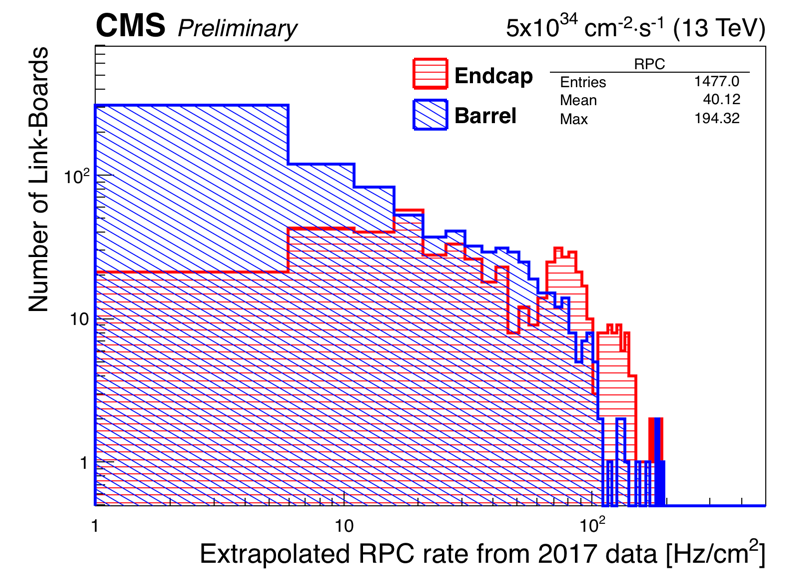
\includegraphics[height=5cm]{fig/chapt5/RPC-Rate-HL-LHC_2017.png}
			\caption{\label{fig:RPC-HL-LHC:A}}
		\end{subfigure}
		\begin{subfigure}{0.5\linewidth}
			\centering
			\includegraphics[height=5cm]{fig/chapt5/RPC-IC-HL-LHC_2016.png}
			\caption{\label{fig:RPC-HL-LHC:B}}
		\end{subfigure}
		\caption{\label{fig:RPC-HL-LHC} Figure~\ref{fig:RPC-HL-LHC:A}: The hit rate per region (Barrel, Endcap) is linearly extrapolated to HL-LHC highest instantaneous luminosity (\Sci{5}{34} \siflux) using the rate as a function of instantaneous luminosity recorded by RPCs in 2017 showing a linear dependence. Figure~\ref{fig:RPC-HL-LHC:B}: The integrated charge per region (Barrel, Endcap) is extrapolated to HL-LHC integrated luminosity (\SI{3000}{fb^{-1}}) using the data accumulated in 2016 in every HV channels.}
	\end{figure}
    
	\begin{figure}[H]
		\begin{subfigure}{0.5\linewidth}
			\centering
			\includegraphics[height=5cm]{fig/chapt5/Mean-Int-charge-Barrel.png}
			\caption{\label{fig:Mean-Int-Charge:A}}
		\end{subfigure}
		\begin{subfigure}{0.5\linewidth}
			\centering
			\includegraphics[height=5cm]{fig/chapt5/Mean-Int-charge-Endcap.png}
			\caption{\label{fig:Mean-Int-Charge:B}}
		\end{subfigure}
		\caption{\label{fig:Mean-Int-Charge} CMS RPC mean integrated charge in the Barrel region (Figure~\ref{fig:Mean-Int-Charge:A}) and the Endcap region (Figure~\ref{fig:Mean-Int-Charge:B}). The integrated charge per year is shown in blue. The red curve shows the evolution of the accumulated integrated charge through time. The blank period in 2013 and 2014 corresponds to LS1. The total integrated charge for the entire operation period (Oct.2009 - Dec.2017) is estimated to be about \SI{1.66}{mC/cm^2} in the Barrel and \SI{4.58}{mC/cm^2} in the Endcap.}
	\end{figure}

	In the past, extensive long-term tests were carried out at several gamma and neutron facilities certifying the detector performance. Both full size and small prototype RPCs have been irradiated with photons up to an integrated charge of $\sim$\SI{0.05}{C/cm^2} and $\sim$\SI{0.4}{C/cm^2} respectively and were certified for rates reaching \SIrate{200}~\cite{GIF2004,AGING2009}. Since the beginning of Run-I until December 2017, the RPC system provided stable operation and excellent performance and did not show any ageing effects for a maximum integrated charge in a detector of the order of \SI{0.01}{C/cm^2} - the average being of the order of \SI{2}{mC/cm^2} in the Barrel and \SI{5}{mC/cm^2} in the Endcap, closer to the beam line, as can be seen from Figure~\ref{fig:Mean-Int-Charge} - and a peak luminosity reaching \Sci{1.4}{34} \siflux during 2017 data taking period.
	
	To perform the necessary studies on the present CMS RPC detectors, facilities offering the possibility to irradiate the chambers are necessary in order to recreate HL-LHC conditions or stronger and study their performance through time. Such facilities exist at CERN and were exploited to conduct this study. A first series of preliminary studies were conducted in the former gamma facility of CERN (GIF) before its dismantlement. This preliminary study was used as a stepping stone towards the building of a more powerful irradiation fully dedicated to longevity studies of CMS and ATLAS subsystems in the perspective of HL-LHC. The period of preliminary work has also been a key moment in the elaboration and improvement of data acquisition, offline analysis and online monitoring tools that are extensively used in the new gamma irradiation facility.
	
		\subsection{GIF}
		\label{chapt5:ssec:GIF}
	
	\begin{figure}[H]
		\centering
		\includegraphics[width = \plotwidth]{fig/chapt5/GIF-Layout.pdf}\\
		\caption{\label{fig:GIFLayout} Layout of the test beam zone called X5c GIF at CERN. Photons from the radioactive source produce a sustained high rate of random hits over the whole area. The zone is surrounded by \SI{8}{m} high and \SI{80}{cm} thick concrete walls. Access is possible through three entry points. Two access doors for personnel and one large gate for material. A crane allows installation of heavy equipment in the area.}
	\end{figure}
		
	Located in the SPS West Area at the downstream end of the X5 test beam, the \acf{GIF} was a test area in which particle detectors were exposed to a particle beam in presence of an adjustable gamma background~\cite{AGOSTEO1999}. Its goal was to reproduce background conditions these detectors would suffer in their operating environment at LHC. GIF layout is showed in Figure ~\ref{fig:GIFLayout}. Gamma photons are produced by a strong $^{137}$Cs source installed in the upstream part of the zone inside a lead container. The source container includes a collimator, designed to irradiate a \SIsurface{6}{6}{m} area at \SI{5}{m} maximum to the source. A thin lens-shaped lead filter helps providing with a uniform out-coming flux in a vertical plane, orthogonal to the beam direction. The photon rate is controlled by further lead filters allowing the maximum rate to be limited and to vary within a range of four orders of magnitude. Particle detectors under test are then placed within the pyramidal volume in front of the source, perpendicularly to the beam line in order to profit from the homogeneous photon flux. Adjusting the background flux of photons can then be done by using the filters and choosing the position of the detectors with respect to the source.
			
	As described on Figure~\ref{fig:CsSource}, the $^{137}$Cs source emits a \SI{662}{keV} photon in 85\% of the decays. An activity of \SI{740}{GBq} was measured on the \Th{5} of March 1997. To estimate the strength of the flux in 2014, was considered the nuclear decay through time associated to the Cesium source whose half-life is well known ($t_{1/2}=$ \SIerror{30.05}{0.08}{y}). The GIF tests where done in between the \Th{20} and the \St{31} of August 2014, i.e. at a time $t=$ \SIerror{17.47}{0.02}{y} resulting in an attenuation of the activity from \SI{740}{GBq} in 1997 to \SI{494}{GBq} in 2014.

	\begin{figure}[H]
		\centering
		\includegraphics[width = \plotwidth]{fig/chapt5/Cs137.pdf}\\
		\caption{\label{fig:CsSource} $^{137}$Cs decays by $\beta^-$ emission to the ground state of $^{137}$Ba (BR = 5.64\%) and via the \SI{662}{keV} isomeric level of $^{137}$Ba (BR = 94.36\%) whose half-life is 2.55min.}
	\end{figure}
		
		\subsection{GIF++}
		\label{chapt5:ssec:GIF++}
		
	The \acf{GIF++}, located in the SPS North Area at the downstream end of the H4 test beam, has replaced its predecessor during LS1 and has been operational since spring 2015~\cite{JAKEL2014}. Like GIF, GIF++ features a $^{137}$Cs source of \SI{662}{keV} gamma photons, their fluence being controlled with a set of filters of various attenuation factors. The source provides two separated large irradiation areas for testing several full-size muon detectors with continuous homogeneous irradiation, as presented in Figure~\ref{fig:GIFpp-Layout}.
	
	 The source activity was measured to be about \SI{13.5}{TBq} in March 2016. The photon flux being far greater than HL-LHC expectations, GIF++ provides an excellent facility for accelerated ageing tests of muon detectors. The source is situated in a bunker designed to perform irradiation test along a muon beam line, the muon beam being available during selected periods throughout the year. The H4 beam, providing the area with muons with a maximum momentum of about \SI{150}{GeV/c}, passes through the GIF++ zone and is used to periodically study the performance of the detectors placed under continuous irradiation. Its flux is of \SI{104}{particles/s/\square\cm} focused in an area similar to \SIsurface{10}{10}{cm}. Therefore, with properly adjusted filters, one can simulate the background expected at HL-LHC and study the performance and ageing of muon detectors in HL-LHC environment.\\
	
	\begin{figure}[H]
		\centering
		\includegraphics[width = 0.8\plotwidth]{fig/chapt5/GIFpp-Layout.png}\\
		\caption{\label{fig:GIFpp-Layout} Floor plan of the GIF++ facility. When the facility downstream of the GIF++ takes electron beam, a beam pipe is installed along the beam line (z-axis). The irradiator can be displaced laterally (its center moves from $x=$ \SI{0.65}{m} to \SI{2.15}{m}), to increase the distance to the beam pipe.}
	\end{figure}
	 
	\begin{figure}[H]
		\begin{subfigure}{0.5\linewidth}
		    \centering
			\includegraphics[width = 0.6\plotwidth]{fig/chapt5/GIFpp-gCurrent-XZ.png}\\
			\caption{\label{fig:GIFpp-gCurrent:XZ}}
		\end{subfigure}
		\begin{subfigure}{0.5\linewidth}
		    \centering
			\includegraphics[width = 0.6\plotwidth]{fig/chapt5/GIFpp-gCurrent-YZ.png}
			\caption{\label{fig:GIFpp-gCurrent:YZ}}
		\end{subfigure}
		\caption{\label{fig:GIFpp-gCurrent} Simulated unattenuated current of photons in the xz plane (Figure~\ref{fig:GIFpp-gCurrent:XZ}) and yz plane (Figure~\ref{fig:GIFpp-gCurrent:YZ}) through the source at $x=$ \SI{0.65}{m} and $y=$ \SI{0}{m}. With angular correction filters, the current of \SI{662}{keV} photons is made uniform in xy planes.}
    \end{figure}
	 
\section{Preliminary studies at GIF}
\label{chapt5:sec:GIFtests}

	\subsection{RPC test setup}
	\label{chapt5:ssec:RPCSetup}
	
	During summer 2014, preliminary tests have been conducted in the GIF area on an endcap chamber of type RE4/2 and labeled \texttt{RE-4-2-BARC-161} produced for the extension of the endcap with a fouth disk in 2013. This chamber has been placed into a trolley covered with a tent. The position of the RPC inside the tent and of the tent with respect to the source in the bunker are described in Figure~\ref{fig:GIFSetup}. The goal of the study were to have a preliminary understanding of the rate capability of the present technology used in CMS. It was decided to measure the efficiency of the RPC under irradiation at detecting cosmic muons as, at the time of the tests, the beam not operational anymore. Three different absorber settings were used and compared to the case where the detector was not irradiated in order to study the evolution of the performance of the detector with increasing exposition to gamma radiation. First of all, measurements were done with fully opened source. To complete this preliminary study, the gamma flux has been attenuated by a factor 2, a factor 5 and finally the source was shut down. Was measured the efficiency of the RPC at detecting the cosmic muons in coincidence with a cosmic trigger as well as the background rate as seen by the detectors.

	\begin{figure}[H]
		\begin{subfigure}{0.5\linewidth}
		    \centering
			\includegraphics[width = 0.5\plotwidth]{fig/chapt5/GIF-Setup-A.pdf}
			\caption{\label{fig:GIFSetup:A}}
		\end{subfigure}
		\begin{subfigure}{0.5\linewidth}
		    \centering
			\includegraphics[width = 0.5\plotwidth]{fig/chapt5/GIF-Setup-B.pdf}
			\caption{\label{fig:GIFSetup:B}}
		\end{subfigure}
		\caption{\label{fig:GIFSetup} Description of the RPC setup. Dimensions are given in \si{mm}. A tent containing RPCs is placed at \SI{1720}{mm} from the source container. The source is situated in the center of the container. RE-4-2-BARC-161 chamber is \SI{160}{mm} inside the tent. This way, the distance between the source and the chambers plan is \SI{2060}{mm}. Figure~\ref{fig:GIFSetup:A} provides a side view of the setup in the $xz$ plane while Figure~\ref{fig:GIFSetup:B} shows a top view in the $yz$ plane.}
	\end{figure}
	
	The trigger system was composed of 2 plastic scintillators and was placed in front of the setup with an inclination of \SI{10}{\degree} with respect to the detector plane in order to look at cosmic muons. Using this particular trigger layout, showed in Figure~\ref{fig:GIF-RPCSetup}, leads to a cosmic muon hit distribution into the chamber similar to the one of Figure~\ref{fig:HitProf}. Measured without gamma irradiation, two peaks can be seen on the profile of readout partition B, centered on strips 52 and 59. Section~\ref{chapt5:ssec:GeoAcc} will help us understand that these two peaks are due respectively to forward and backward coming cosmic particles where forward coming particles are first detected by the scintillators and then the RPC while the backward coming muons are first detected in the RPC.

	\begin{figure}[H]
		\centering
		\includegraphics[width = 0.8\plotwidth]{fig/chapt5/GIF-RPCSetup.jpg}\\
		\caption{\label{fig:GIF-RPCSetup} \texttt{RE-4-2-BARC-161} chamber is inside the tent as described in Figure~\ref{fig:GIFSetup}. In the top right, the two scintillators used as trigger can be seen. This trigger system has an inclination of \SI{10}{\degree} relative to horizontal and is placed above half-partition B2 of the RPCs. PMT electronics are shielded thanks to lead blocks placed in order to protect them without stopping photons from going through the scintillators and the chamber.}
	\end{figure}

		\begin{figure}[H]
		\centering
		\includegraphics[width = 0.7\plotwidth]{fig/chapt5/Data-21-profile.pdf}\\
		\caption{\label{fig:HitProf} Hit distributions over all 3 partitions of \texttt{RE-4-2-BARC-161} chamber is showed. Top, middle and bottom figures respectively correspond to partitions A, B, and C. The profiles show that some events still occur in other half-partitions than B2, which corresponds to strips 49 to 64, in front of which the trigger is placed, contributing to the inefficiency of detection of cosmic muons. In the case of partitions A and C, the very low amount of data can be interpreted as noise. On the other hand, it is clear that a little portion of muons reach the half-partition B1, corresponding to strips 33 to 48.}
	\end{figure}
	
	The data taking is then performed thanks to a \texttt{CEAN} TDC module of type \texttt{V1190A}~\cite{V1190AMUT} to which is connected the digitized output of the RPC \acl{FEB}, as described in Figure~\ref{fig:DAQ:A} and the trigger signal from the telescope. The communication with the computer is performed thanks to a \texttt{CAEN} communication module of type \texttt{V1718}~\cite{V1718MUT}. In order to control the rates recorded by the detector, the digitized RPC signals are also sent to scalers as described in Figure~\ref{fig:DAQ:B}. The \texttt{C++} DAQ software used in GIF was developed as an early attempt towards the understanding of the \texttt{CAEN} libraries and the data collected by the TDCs was saved into \texttt{.dat} files is analysed with an algorithm computing parameters such as efficiency, hit profile, cluster size, or gamma and noise rates which was developed with \texttt{C++} as well. Finally, histograms and curves are produced using \texttt{ROOT}.

	\begin{figure}[H]
		\begin{subfigure}{\linewidth}
			\centering
			\includegraphics[width = \plotwidth]{fig/chapt5/pulse-processing.pdf}\\
			\caption{\label{fig:DAQ:A}}
		\end{subfigure}
		\begin{subfigure}{\linewidth}
			\centering
			\includegraphics[width = \plotwidth]{fig/chapt5/pulse-processing-2.pdf}
			\caption{\label{fig:DAQ:B}}
		\end{subfigure}
		\caption{\label{fig:DAQ} Signals from the RPC strips are shaped by the FEE described on Figure ~\ref{fig:DAQ:A}. Output LVDS signals are then read-out by a TDC module connected to a computer or converted into NIM and sent to scalers. Figure~\ref{fig:DAQ:B} describes how these converted signals are put in coincidence with the trigger.}
	\end{figure}
	
	\subsection{Geometrical acceptance of the setup layout to cosmic muons}
	\label{chapt5:ssec:GeoAcc}
				
	In order to profit from a constant gamma irradiation, the detectors inside of the GIF bunker need to be placed in a plane orthogonal to the beam line. The muon beam that used to be available was meant to test the performance of detectors under test. This beam not being active anymore, an other solution to test detector performance had to be used. Thus, it has been decided to use cosmic muons detected through a telescope composed of two scintillators. Lead blocks were used as shielding to protect the photomultipliers from gammas as can be seen from Figure~\ref{fig:GIF-RPCSetup}.
				
	An inclination of $\sim$\SI{10}{\degree} has been given to the cosmic telescope to maximize the muon flux. A good compromise had to be found between good enough muon flux and narrow enough hit distribution to be sure to contain all the events into only one half partitions as required from the limited available readout hardware. It was then foreseen to detect muons and read them out only from half-partition B2, the last 16 channels of readout partition B (i.e. strips 49 to 64). Nevertheless, a consequence of the misplaced trigger, that can be seen as a loss of events in half-partition B1 (strips 33 to 48) in Figure~\ref{fig:HitProf}, is an inefficiency. The observed inefficiency of approximately 20\% highlighted in Figure~\ref{fig:EffCompar} by comparing the performance of chamber \texttt{RE-4-2-BARC-161} as measured prior to the study at GIF and at GIF without irradiation seems too important, compared to the 12.7\% of data contained into the first 16 strips observed on Figure~\ref{fig:HitProf}, to only be explained by the geometrical acceptance of the setup itself. Simulations have been conducted to show how the setup brings inefficiency.

	\begin{figure}[H]
            \centering
		\includegraphics[width = \plotwidth]{fig/chapt5/Compared-Efficiency.pdf}
		\caption{\label{fig:EffCompar} Results are derived from data taken on half-partition B2 only. On the \Th{18} of June 2014, data has been taken on chamber \texttt{RE-4-2-BARC-161} at CERN building 904 (Prevessin Site) with cosmic muons providing us a reference efficiency plateau of \numerror{97.54}{0.15}\% represented by a black curve. A similar measurement has been done at GIF on the \St{21} of July with the same chamber giving a plateau of \numerror{78.52}{0.94}\% represented by a red curve.}
	\end{figure}
	
		\subsubsection{Description of the simulation layout}
		\label{chapt5:sssec:SimLayout}
		
	The layout of GIF setup has been reproduced, only roughly using Figure~\ref{fig:GIF-RPCSetup} due to the lack of measures, and incorporated into a \texttt{C++} \acf{MC} simulation to study the geometrical acceptance of the telescope projected onto the readout strips~\cite{GEOACCEPT}. A 3D view of the simulated layout is given into Figure~\ref{fig:SimGIFLay}. Muons are generated randomly in a horizontal plane located at a height corresponding to the lowest point of the PMTs. This way, the needed size of the plane in order to simulate events happening at very large azimuthal angles (i.e. $\theta\approx\pi$) can be kept relatively small while the total number of muon tracks to propagate is kept relatively small. The muon flux is designed to follow the usual $cos^2\theta$ distribution for cosmic particles. The goal of the simulation is to look at muons that pass through the telescope composed of the two scintillators and define their distribution onto the RPC read-out plane. During the reconstruction, the read-out plane is then divided into read-out strips and each muon track is assigned to a strip.

	\begin{figure}[H]
		\begin{subfigure}{\linewidth}
			\centering
			\includegraphics[width = 0.8\plotwidth]{fig/chapt5/GIFSetup-SimA.png}\\
			\caption{\label{fig:SimGIFLay:A}}
		\end{subfigure}
		\begin{subfigure}{\linewidth}
			\centering
			\includegraphics[width = 0.8\plotwidth]{fig/chapt5/GIFSetup-SimB.png}
			\caption{\label{fig:SimGIFLay:B}}
		\end{subfigure}
		\caption{\label{fig:SimGIFLay} Representation of the layout used for the simulations of the test setup. The RPC read-out plane is represented as a yellow trapezoid while the two scintillators as blue cuboids looking at the sky. The green plane corresponds to the muon generation plane within the simulation. Figure~\ref{fig:GIFSetup:A} shows a global view of the simulated setup. Figure~\ref{fig:GIFSetup:B} shows a zoomed view that allows to see the 2 scintillators as well as the full RPC plane.}
	\end{figure}
		
		\subsubsection{Simulation procedure}
		\label{chapt5:sssec:SimProc}
		
	$N_{\mu}=$ \Ord{8} muons are randomly generated inside the muon plane with an azimutal angle $\theta$ chosen to follow a $cos^2\theta$ distribution. Infinite planes are associated to each surface of the scintillators. Knowing the muon position into the muon generation plane and its direction allows, by assuming that muons travel in a straight line, to compute the intersection of the muon track with these planes. Applying conditions to the limits on the contours of the scintillators' faces then gives an answer to weither or not the muon passed through the scintillators. In the case the muon was not \textit{detected} into both scintillators, the simulation discards the muon and generates a new one.
	
	On the contrary, if the muon is labeled as good, its position within the RPC read-out plane is computed and the corresponding strip, determined through geometrical tests, gets a \textit{hit}. Muon hits fill different histograms weither they are associated to forward or backward coming muons. A discrimination is performed according to their direction components. An $(x,y,z)$ position  into the generation plane as well as a ($\theta$;$\phi$) pair are associated to each generated muon providing with information on the direction the track follows. This way, muons satisfying the condition $0\leq\phi<\pi$ are labeled as \textit{backward} coming muons while muons satisfying $\pi\leq\phi<2\pi$ as \textit{forward} coming muons.
		
		\subsubsection{Results and limitations}
		\label{chapt5:sssec:SimRes}
	
	The output from the simulation is given in Figure~\ref{fig:SimResult} in which the distribution is showed for all muons but also for the separate contributions of forward and backward coming muons. The strip number is here given in a range of 1 to 32 corresponding to the 32 strips contained in each RPC read-out partition, without taking into account the fact that partition B of an RPC correponds, by convention, to strips 33 to 64. Comparing the number of muons recoreded respectively in the first 16 strips and the in all of the 32 strips of the RPC read-out panel, it can be established than, out of the total amount of muons that have passed through the telescope and reached the RPC, 16.8\% where to be detected in the 16 first strip of the read-out plane corresponding to half partition B1. This brings a geometrical inefficiency of the same amount that can then be used to correct the data by scaling up by a factor $c_{geo} = 1/(1-0.168)$ the maximum efficiency measured during data taking.

	\begin{figure}[H]
		\begin{subfigure}{\linewidth}
			\centering
			\includegraphics[width = 0.6\plotwidth]{fig/chapt5/Geometrical-acceptance.pdf}\\
			\caption{\label{fig:SimResult:A} Full acceptance distribution}
		\end{subfigure}
		\begin{subfigure}{0.5\linewidth}
			\centering
			\includegraphics[width = 0.6\plotwidth]{fig/chapt5/Geometrical-acceptance-forward.pdf}
			\caption{\label{fig:SimResult:B} Forward acceptance}
		\end{subfigure}
		\begin{subfigure}{0.5\linewidth}
			\centering
			\includegraphics[width = 0.6\plotwidth]{fig/chapt5/Geometrical-acceptance-backward.pdf}
			\caption{\label{fig:SimResult:C} Backward acceptance}
		\end{subfigure}
		\caption{\label{fig:SimResult} Geometrical acceptance distribution as provided by the \acl{MC} simulation.}
	\end{figure}
	
	Nevertheless, it is difficult to evaluate a systematical uncertainty on this geometrical correction for different reasons. First of all, eventhough the dimensions of the scintillators and of the RPC are well known, the position of each element of the setup with respect to one another was not measured. It was then necessary, using known dimensions, to extract the positions of each element from Figure~\ref{fig:GIF-RPCSetup} with unknown uncertainty. The inclination is also roughly measured to be \SI{10}{\degree} and even if the position of each peak, distant in the simulation of 7 strips, tends to confirm this assumption, the geometrical inefficiency would be affected by a variation of the inclination angle. Introducing in the simulation an error of $\pm$\SI{2}{\degree} would lead to a correction factor $c_{geo} = 1.20^{+0.04}_{-0.03}$ that allows for a good improvement of the efficiency measured in GIF, as can be seen from Figure~\ref{fig:EffCorrection}. GIF measurement is in agreement with the reference curve within statistical errors.

	\begin{figure}[H]
            \centering
		\includegraphics[width = \plotwidth]{fig/chapt5/Compared-Efficiency-Correction.pdf}
		\caption{\label{fig:EffCorrection} Correction of the efficiency without source. The efficiency after correction gets much closer to the Reference measurement performed before the study in GIF by reaching a plateau of \numerror{93.52}{2.64}\%.}
	\end{figure}
	
	Further corrections could be also be brought as it can easily be understood that the distribution showed through Figure~\ref{fig:SimResult:A} differs from the measured hit profile showed in Figure~\ref{fig:HitProf}. The contributions of forward and backward muon indicate that 28.1\% of the total geometrical acceptance should contribute to detecting backward muons whereas it is measured that the hit profile contains 22.0\% of backward data only. This estimation of the backward versus forward content in the data was done through a fit using a sum of two skew distribution, one acting on the forward muon peak while the other acts on the backward muon fit, as showed in Figure~\ref{fig:Fit-data}. Although a skew distribution lacks physical interpretation, it allows to easily fit such kind of data. A description of a skew distribution, as the product of a gaussian and a sigmoid (Formula~\ref{eq:gaus-sig}), is given through Formula~\ref{eq:skew}.
	
	\begin{equation}
	\label{eq:gaus-sig}
	g(x) = A_g e^{\frac{-(x-\bar{x})^2}{2\sigma^2}}\; , \quad s(x) = \frac{A_s}{1+e^{-\lambda(x-x_i)}}
	\end{equation}
	
	\begin{equation}
	\label{eq:skew}
	sk(x) = g(x)\times s(x) = A_{sk}\frac{e^{\frac{-(x-\bar{x})^2}{2\sigma^2}}}{1+e^{-\lambda(x-x_i)}}
	\end{equation}

	\begin{figure}[H]
            \centering
		\includegraphics[width = 0.7\plotwidth]{fig/chapt5/Cosmic-data-21-skew-fit.pdf}
		\caption{\label{fig:Fit-data} Hit distributions over read-out partition B of \texttt{RE-4-2-BARC-161} chamber together with skew distribution fits corresponding to forward and backward coming muons.}
	\end{figure}
	
	From the obvious difference in between geometrical simulation and data, it is necessary to realize that the geometrical acceptance and the hit profile are two dinstinct information. When the geometrical acceptance only provides with the information about what the detector can expect to see in a perfect world where all muons are detected in the exact same way independantly from their energy, angle of incidence, fluctuation of the detector gain due to complexe avalanche development, thresholds applied on the scintillators and on the RPC FEEs to reduce the noise, the cross-talk and corresponding spread of the induced charge observed on the read-out strips, the hit profile provides the final product of all the previously mentioned contributions and can greatly differ from purely geometrical considerations. A full physics analysis involving softwares such as \texttt{GEANT} would be required to further refine the correction on the measured efficiency at GIF.
	
	\subsection{Photon flux at \acs{GIF}}
	\label{chapt5:ssec:gFlux}
		
	In order to understand and evaluate the $\gamma$ flux in the GIF area, simulations had been conducted at the time GIF was opened for research purposes~\cite{AGOSTEO1999}. Table~\ref{tab:Sim1997} presented in this article gives the $\gamma$ flux for different distances $D$ to the source. The simulation was done using GEANT and a \acf{MCNP} transport code, and the flux $F$ is given with the estimated error from these packages expressed in \%.
	
	\begin{table}[H]
		\centering
		\begin{tabular}{|*{5}{c|}}
			\hline
			Nominal & \multicolumn{4}{c|}{Photon flux $F$ [\siflux]} \\
			\cline{2-5}
			ABS & at $D=$ \SI{50}{cm} & at $D=$ \SI{155}{cm} & at $D=$ \SI{300}{cm} & at $D=$ \SI{400}{cm} \\
			\hline
			1 & \Sci{0.12}{8} $\pm$ 0.2\% & \Sci{0.14}{7} $\pm$ 0.5\% & \Sci{0.45}{6} $\pm$ 0.5\% & \Sci{0.28}{6} $\pm$ 0.5\% \\
			\hline
			2 & \Sci{0.68}{7} $\pm$ 0.3\% & \Sci{0.80}{6} $\pm$ 0.8\% & \Sci{0.25}{6} $\pm$ 0.8\% & \Sci{0.16}{6} $\pm$ 0.6\% \\
			\hline
			5 & \Sci{0.31}{7} $\pm$ 0.4\% & \Sci{0.36}{6} $\pm$ 1.2\% & \Sci{0.11}{6} $\pm$ 1.2\% & \Sci{0.70}{5} $\pm$ 0.9\% \\
			\hline
		\end{tabular}
		\caption{\label{tab:Sim1997} Total photon flux ($E\gamma \leq$ \SI{662}{keV}) with statistical error predicted considering a $^{137}$Cs activity of \SI{740}{GBq} at different values of the distance $D$ to the source along the x-axis of irradiation field~\cite{AGOSTEO1999}.}
	\end{table}
	
	The simulation does not provide with an estimated flux at the level of the RPC under test. First of all, it is necessary to extract the value of the flux from the available data contained in the original paper and then to estimate the flux in 2014 at the time the experimentation took place. In the case of a pointlike source emiting isotrope and homogeneous gamma radiations, the gamma flux $F$ at a distance $D$ from the source with respect to a reference point situated at $D_0$ where a known flux $F_0$ is measured will be expressed like in Formula~\ref{eq:Flux}, assuming that the flux decreases as $1/D^2$, where $c$ is a fitting factor that can be written from Formula~\ref{eq:Flux} as Formula~\ref{eq:Factor}. Finally, using Equation~\ref{eq:Factor} and the data of Table~\ref{tab:Sim1997}, with $D_0=$ \SI{50}{cm} as reference point, Table~\ref{tab:CorrFactor} can be built. It is interesting to note that $c$ for each value of $D$ doesn't depend on the absorption factor.
	
	\begin{equation}
	\label{eq:Flux}
	F^{ABS} = F_0^{ABS} \times \left( \frac{c D_0}{D} \right)^2
	\end{equation}
	
	\begin{equation}
	\label{eq:Factor}
	c = \frac{D}{D_0}\sqrt{\frac{F^{ABS}}{F_0^{ABS}}} \; , \quad \Delta c = \frac{c}{2}\left(\frac{\Delta F^{ABS}}{F^{ABS}}+\frac{\Delta F^{ABS}_0}{F^{ABS}_0}\right)
	\end{equation}
	
	\begin{table}[H]
		\centering
		\begin{tabular}{|*{4}{c|}}
			\hline
			Nominal & \multicolumn{3}{c|}{Correction factor $c$} \\
			ABS & at $D=$ \SI{155}{cm} & at $D=$ \SI{300}{cm} & at $D=$ \SI{400}{cm} \\
			\hline
			1 & $1.059 \pm 0.70\%$ & $1.162 \pm 0.70\%$ & $1.222 \pm 0.70\%$ \\
			\hline
			2 & $1.063 \pm 1.10\%$ & $1.150 \pm 1.10\%$ & $1.227 \pm 0.90\%$ \\
			\hline
			5 & $1.056 \pm 1.60\%$ & $1.130 \pm 1.60\%$ & $1.202 \pm 1.30\%$ \\
			\hline
		\end{tabular}
		\caption{\label{tab:CorrFactor} Correction factor c is computed thanks to Formula~\ref{eq:Factor} taking as reference $D_0 =$ \SI{50}{cm} and the associated flux $F_0^{ABS}$ for each absorption factor available in table~\ref{tab:Sim1997}.}
	\end{table}
	
	For the range of $D/D_0$ values available, it is possible to use a simple linear fit to get the evolution of $c$ that can be expressed as $c(D/D_0)=aD/D_0+b$. Using Formula~\ref{eq:FluxLinearAp}, but neglecting the incertainty on $D$ that will only be used when extrapolating the values for the position of the RPC under test whose position is not perfectly known, the results showed in Figure~\ref{fig:CorrFactor} is obtained. Figure~\ref{fig:CorrFactor:B} confirms that using only a linear fit to extract $c$ is enough as the evolution of the rate that can be obtained superimposes well on the simulation points.
	
	\begin{equation}
	\label{eq:FluxLinearAp}
	F^{ABS} = F^{ABS}_0 \left( a + \frac{bD_0}{D} \right)^2 \; , \quad \Delta F^{ABS} = F^{ABS} \left[\frac{\Delta F^{ABS}_0}{F^{ABS}_0} + 2\frac{\Delta a + \Delta b\frac{D_0}{D} + \Delta D\frac{bD_0}{D^2}}{a + \frac{bD_0}{D}}\right]
	\end{equation}
	
	In the context of the 2014 GIF tests, the RPC read-out plane is located at a distance $D=$ \SI{206}{cm} from the source. Moreover, to estimate the strength of the flux in 2014 it is necessary to consider the nuclear decay through time assiciated to the Cesium source whose half-life is well known ($t_{1/2}=$ \SIerror{30.05}{0.08}{y}). The very first source activity measurement has been done on the \Th{5} of March 1997 while the GIF tests where done in between the \Th{20} and the \Th{31} of August 2014, i.e. at a time $t=$ \SIerror{17.47}{0.02}{y} resulting in an attenuation of the activity from \SI{740}{GBq} in 1997 to \SI{494}{GBq} in 2014. All the needed information to extrapolate the expected flux through the detector at the moment of GIF preliminary tests has now been assembled, leading to Table~\ref{tab:extra2014}. By assuming a sensitivity of the RPC to $\gamma$ of \Sci{2}{-3}, the order of magnitude of the expected hit rate per unit area would be of the order of the \si{kHz} for the fully opened source, as reported in the last column of the table.
	
	\begin{figure}[H]
		\begin{subfigure}{\linewidth}
			\centering
			\includegraphics[width = 0.8\plotwidth]{fig/chapt5/flux_correction.pdf}\\
			\caption{\label{fig:CorrFactor:A}}
		\end{subfigure}
		\begin{subfigure}{\linewidth}
			\centering
			\includegraphics[width = 0.8\plotwidth]{fig/chapt5/correction_model.pdf}
			\caption{\label{fig:CorrFactor:B}}
		\end{subfigure}
		\caption{\label{fig:CorrFactor} Figure~\ref{fig:CorrFactor:A} shows the linear approximation fit performed on data extracted from table~\ref{tab:CorrFactor}. Figure~\ref{fig:CorrFactor:B} shows a comparison of Formula~\ref{eq:FluxLinearAp} with the simulated flux using $a$ and $b$ given in figure~\ref{fig:CorrFactor:A} in formulae ~\ref{eq:Flux} and the reference value $D_0 =$ \SI{50}{cm} and the associated flux for each absorption factor $F_0^{ABS}$ from table~\ref{tab:Sim1997}}
	\end{figure}
	
	\begin{table}[H]
		\begin{tabular}{|*{5}{c|}}
			\hline
			Nominal & \multicolumn{3}{c|}{Photon flux $F$ [\siflux]} & Rate [\sirate] \\
			ABS & at $D_0^{97}=$ \SI{50}{cm} & at $D^{97}=$ \SI{206}{cm} & at $D^{2014}=$ \SI{206}{cm} & at $D^{2014}=$ \SI{206}{cm} \\
			\hline
			1 & \Sci{0.12}{8} $\pm$ 0.2\% & \Sci{0.84}{6} $\pm$ 1.2\% & \Sci{0.56}{6} $\pm$ 1.2\% & $1129 \pm 14$ \\
			\hline
			2 & \Sci{0.68}{7} $\pm$ 0.3\% & \Sci{0.48}{6} $\pm$ 1.2\% & \Sci{0.32}{6} $\pm$ 1.2\% & $640 \pm 8$ \\
			\hline
			5 & \Sci{0.31}{7} $\pm$ 0.4\% & \Sci{0.22}{6} $\pm$ 1.2\% & \Sci{0.15}{6} $\pm$ 1.2\% & $292 \pm 4$ \\
			\hline
		\end{tabular}
		\caption{\label{tab:extra2014} The data at $D_0$ in 1997 is taken from~\cite{AGOSTEO1999}. Using Formula~\ref{eq:FluxLinearAp}, the flux at $D$, including an error of \SI{1}{cm}, can be estimated in 1997. Then, taking into account the attenuation of the source activity, the flux at $D$ can be estimated at the time of the tests in GIF in 2014. Assuming a sensitivity of the RPC to $\gamma$ $s =$ \Sci{2}{-3}, an estimation of the hit rate per unit area is obtained.}
	\end{table}
	
	The goal of the study will be to have a good measurement of the intrinsic performance without source irradiation. Then, taking profit of the two working absorbers, at absorbtion factors 5 (\SI{300}{Hz}) and 2 ($\sim$\SI{600}{Hz}) the goal will be to show that the detectors fulfill the performance certification of CMS RPCs. Finally, a first idea of the performance of the detectors at higher background will be provided with absorbtion factor 1 (no absorbtion and $>$\SI{1}{kHz})).
	
	\subsection{Results and discussions}
	\label{chapt5:ssec:resultsGIF}
	
	The data taking at GIF has been conducted in between the \St{21} and the \St{31} of August, 2014. Data has been collected with both source OFF and ON using three different absorber settings (ABS 5, 2 and 1) in order to vary the irradiation on the RPC. For each source setting, two HV scans have been performed with two different trigger settings. During a first scan the trigger sent to the TDC module was the coincidence of the two scintillators composing the telescope while during a second scan the trigger was a pulse coming from a pulse generator in order to measure the noise or gamma rate seen by the chamber. Indeed, using a pulse allows to trigger at moments not linked to any physical event and, hence, to obtain a \textit{RANDOM} trigger on noise and gamma events to measure the associated rates, the probability to have a pulse in coincidence with a cosmic muon being negligible.
	
	From the cosmic trigger scans, a summary of the effiencies and corresponding cluster sizes is showed in Figure~\ref{fig:GIFEffCS}. The efficiency curves with Source ON show a shift with respect to the case without irradiation. With ABS 5, the general shape of the efficiency curve stays unchanged whereas a clear alteration of the performance is observed at ABS 2 and ABS 1. From the cluster size results, a reduction of the cluster size under irradiation can be oberved at equivalent efficiency. This effect can be due to the perturbation of the electric field by the strong rate of gamma particles starting avalanches in the gas volume of the detector.
	
	\begin{figure}[H]
    	\begin{subfigure}{0.5\linewidth}
			\centering
			\includegraphics[width = 0.7\plotwidth]{fig/chapt5/Efficiency.pdf}
        	\caption{\label{fig:GIFEffCS:A}}
    	\end{subfigure}
    	\begin{subfigure}{0.5\linewidth}
			\centering
			\includegraphics[width = 0.7\plotwidth]{fig/chapt5/Cluster-Size.pdf}
        	\caption{\label{fig:GIFEffCS:B}}
    	\end{subfigure}
		\caption{\label{fig:GIFEffCS} Efficiency (Figure~\ref{fig:GIFEffCS:A}) and cluster size (Figure~\ref{fig:GIFEffCS:B}) of chamber \texttt{RE-4-2-BARC-161} measured at GIF with Source OFF (red) and Source ON using different absorber settings: ABS 5 (green), ABS 2 (blue) and ABS 1 (yellow). The results are compared to the Reference values obtained with cosmics.}
	\end{figure}
	
	It is necessary to study the evolution of the performance of the chamber with the increasing rate. In Figure~\ref{fig:GIFRate:A}, the noise rate when the source is OFF stays low but increases at voltages above \SI{9500}{V}. The rise of the noise rate in the detector can be related to the increased streamer probability observed with such a large electric field. The rates with source ON measured at GIF all show a similar behaviour until a high voltage of approximately \SI{9400}{V} at which the rate of ABS 5 saturates, corresponding to the chamber reaching full efficiency. It is important to note that, eventhough the rates look similar independently from the gamma flux, relatively to the efficiency of the chamber, the rate actually increases with increasing flux at equivalent efficiency. A rough way to measure the rate effectively observed by the detector for each source setting would be to normalize the measured rates to the efficiency of the detector. This exercise was done with Figure~\ref{fig:GIFRate:B} from which constant fits where done on Source ON data in order to extract the rate the chamber was subjected to.
	
	\begin{figure}[H]
    	\begin{subfigure}{0.5\linewidth}
			\centering
			\includegraphics[width = 0.7\plotwidth]{fig/chapt5/Gamma-Rate.pdf}
        	\caption{\label{fig:GIFRate:A}}
    	\end{subfigure}
    	\begin{subfigure}{0.5\linewidth}
			\centering
			\includegraphics[width = 0.7\plotwidth]{fig/chapt5/Unconvoluted-Gamma-Rate.pdf}
        	\caption{\label{fig:GIFRate:B}}
    	\end{subfigure}
		\caption{\label{fig:GIFRate} Rates in chamber \texttt{RE-4-2-BARC-161} measured at GIF with Source OFF (red) and Source ON using different absorber settings: ABS 5 (green), ABS 2 (blue) and ABS 1 (yellow). On Figure~\ref{fig:GIFRate:B}, the rates of Figure~\ref{fig:GIFRate:A} were normalized to the measured efficiency and constant fits are performed on Source ON data showing the gamma rate in the chamber.}
	\end{figure}
	
	\begin{figure}[H]
    	\begin{subfigure}{0.5\linewidth}
			\centering
    		\includegraphics[width = 0.7\plotwidth]{fig/chapt5/HV-Knee-ABS.pdf}
        	\caption{\label{fig:Evolution:A}}
    	\end{subfigure}
    	\begin{subfigure}{0.5\linewidth}
			\centering
    		\includegraphics[width = 0.7\plotwidth]{fig/chapt5/Eff-ABS.pdf}\\
        	\caption{\label{fig:Evolution:B}}
    	\end{subfigure}
		\caption{\label{fig:Evolution} Evolution of the voltages at half maximum and at 95\% of the maximum efficiency (Figure~\ref{fig:Evolution:A}), and of the maximum efficiency (Figure~\ref{fig:Evolution:B}) as a function of the rate in chamber \texttt{RE-4-2-BARC-161}. The data is extracted from the fits in Figures~\ref{fig:GIFEffCS:A} and~\ref{fig:GIFRate:B}.}
	\end{figure}
	
	The results need to be taken with care as a better estimation of the rate would have been to push the detector towards higher voltages to reach the efficiency plateau for each absorber configuration and only then extract the measured rate at working voltage, defined as in Formula~\ref{eq:KneeWP}. Nevertheless, using this method to estimate the rate the chamber is subjected to, it is possible to look at the evolution of the $HV_{50}$ and $HV_{knee}$ (the working voltage being defined to be \SI{150}{V} above the knee in the endcap) as a function of the increasing rate as showed in Figure~\ref{fig:Evolution}. The results from GIF suggest that at a rate of \SIrate{600} the working voltage of the chamber is increased by a thousand \si{V} while the efficiency is reduced to approximately 80\%, although the result still is consistent with an efficiency better than 90\% due to the large error on the measurement. Moreover, it is likely that the rates obtained through fitting on normalized values is underestimated. Indeed, monitoring the current in the 3 gaps composing a CMS endcap RPC (Figure~\ref{fig:EndcapRPC}) while knowing the rate, the charge deposition per avalanche $q_\gamma$ can be computed.
	
	\begin{figure}[H]
    	\begin{subfigure}{0.69\linewidth}
			\centering
    		\includegraphics[height = 5cm]{fig/chapt5/Endcap-3D.pdf}
        	\caption{\label{fig:EndcapRPC:A}}
    	\end{subfigure}
    	\begin{subfigure}{0.29\linewidth}
			\centering
    		\includegraphics[height = 5cm]{fig/chapt5/Endcap-side.pdf}\\
        	\caption{\label{fig:EndcapRPC:B}}
    	\end{subfigure}
		\caption{\label{fig:EndcapRPC} Presentation of a double-gap endcap RPC with its 3 RPC gaps. Due to the partitioniing of the read-out strips into 3 rolls, the TOP layer of gap is divided into 2 gaps: TOP NARROW (TN) and TOP WIDE (TW). The BOTTOM (B) only consists in 1 gap.}
	\end{figure}
	
	A charge is expressed in \si{C} which is consistent with a current density, expressed in \si{A/cm^2}, divided by a rate per unit area, expressed in \si{Hz/cm^2}. The current driven by the RPC is assumed to be due to the irradiation, hence, to the avalanches developing in the gas volume due to the photons of the Cesium source. On the other hand, the rate is supposed to be a measure of the number of photons interacting with the detector. This way, it comes that the charge deposition per avalanche is expressed like $q_\gamma = J_{mon}/R_\gamma$, $J_{mon}$ being the monitored current density and $R_\gamma$ the measured $\gamma$ rate. The current density is computed as the sum of the current density measured on the top gap layer and of which measured in the bottom gap layer, $J_{mon} = (I_{mon}^{TW}+I_{mon}^{TW})/(A_{TW}+A_{TN}) + I_{mon}^B/A_B$, $A_{B,TN,TW}$ being the active area and $I_{mon}^{B,TN,TW}$ the monitored currents of the gaps. According to Figure~\ref{fig:Charge}, the charge deposition per avalanche consistently converges to a value of the order of \SI{50}{pC} for each absorber setting which corresponds to a value more than twice greater than what reported in litterature for CMS detectors~\cite{PUGLIESE2002,PUGLIESE2003} indicating that the rates could have been wrongly evaluated during the short study performed at GIF. An increase of the $\gamma$ rate by a factor 2 would be consistent with the expected rates calculated in Table~\ref{tab:extra2014}, assuming the sensitivity to $\gamma$ to be of the order of \Sci{2}{-3}.
	
	\begin{figure}[H]
    	\begin{subfigure}{0.5\linewidth}
			\centering
    		\includegraphics[width = 0.7\plotwidth]{fig/chapt5/Current-Density.pdf}
        	\caption{\label{fig:Charge:A}}
    	\end{subfigure}
    	\begin{subfigure}{0.5\linewidth}
			\centering
    		\includegraphics[width = 0.7\plotwidth]{fig/chapt5/Charge-per-gamma.pdf}
        	\caption{\label{fig:Charge:B}}
    	\end{subfigure}
		\caption{\label{fig:Charge} Current density and charge deposition per gamma avalanche, defined as the current density normalized to the measured rate taken from Figure~\ref{fig:GIFRate:A} as a function of the effective high voltage in chamber \texttt{RE-4-2-BARC-161} measured at GIF with Source ON using different absorber settings: ABS 5 (green), ABS 2 (blue) and ABS 1 (yellow).}
	\end{figure}
	
	Overall, working at GIF has been a rewarding experience as it offered CMS RPC R\&D team the possibility to start developping the necessary skills and tools that would become the core of GIF++ experiment. The quality of the results can be argued both due to the little robustness of the experimental setup and the lack of available statistics to draw conclusions from, bringing large errors on the final result. The confrontation of the data to known results pointed to a failure in correctly measuring the $\gamma$ rate at working voltage and, hence, to an overestimation of the charge per avalanche and of the drift of working voltage with increasing rate. Nevertheless, the prototypes of DAQ and offline analysis tools proved to be reliable.

\section{Longevity tests at \acs{GIF++}}
\label{chapt5:sec:GIFpptests}

	\subsection{Selection and characterization of CMS RPCs for longevity at GIF++}
	\label{chapt5:ssec:selection}

	First proposed in 2009~\cite{GIF++2009}, the \acl{GIF++} of CERN was thought in the perscpective of future upgrades of PHC that would bring detectors to be operated in a high irradiation environment. GIF++ would thus provide all LHC R\&D teams working on behalf of the different LHC experiment with a facility to perform longevity studies using a very intense Cesium gamma source.
	
	In the specific case of CMS RPC, the longevity studies imply a constant irradiation of selected detectors in order to accumulate a charge equivalent to what is expected during HL-LHC, i.e. a charge of \SI{0.8}{C/cm^2} according to Figure~\ref{fig:RPC-HL-LHC} including a safety factor 3, while other detectors are left non irradiated to be used as references. Throughout the irradiation campaign, the performance of the irradiated and reference detectors will be periodically probed using the high intensity H4 muon beam. Dedicated test beam periods will be used to measure the efficiency and $\gamma$ rate at the level of the detectors with different source absorber settings to have access to the rate capability of CMS RPCs, that needs to be certified above \SIrate{600}, and to identify signs of ageing in the case the performance of the irradiated detectors diverges from those of the reference detectors with increasing accumulated charge. Other than the performance of the detectors, signs of ageing could come from increasing dark current that would be related to local ageing of the electrodes. A close monitoring of the current driven by the detectors will then be necessary as well as dedicated periodical electrode resistivity measurement.
	
	\begin{figure}[H]
    	\begin{subfigure}{0.5\linewidth}
			\centering
    		\includegraphics[width = 0.7\plotwidth]{fig/chapt5/Consolidation-Efficiency.pdf}
        	\caption{\label{fig:consolidation:A}}
    	\end{subfigure}
    	\begin{subfigure}{0.5\linewidth}
			\centering
    		\includegraphics[width = 0.7\plotwidth]{fig/chapt5/Consolidation-Cluster-Size.pdf}
        	\caption{\label{fig:consolidation:B}}
    	\end{subfigure}
    	\begin{subfigure}{0.5\linewidth}
			\centering
    		\includegraphics[width = 0.7\plotwidth]{fig/chapt5/Consolidation-Noise-Rate.pdf}
        	\caption{\label{fig:consolidation:C}}
    	\end{subfigure}
    	\begin{subfigure}{0.5\linewidth}
			\centering
    		\includegraphics[width = 0.7\plotwidth]{fig/chapt5/Consolidation-Current-Density.pdf}
        	\caption{\label{fig:consolidation:D}}
    	\end{subfigure}
		\caption{\label{fig:consolidation} Characterization of CMS RPC detectors foreseen to be used at GIF++ for longevity studies of the present system. Using cosmic muons, efficiency (Figure~\ref{fig:consolidation:A}) and cluster size (Figure~\ref{fig:consolidation:B}) were measured as well as noise rate (Figure~\ref{fig:consolidation:C}) and current density (Figure~\ref{fig:consolidation:D}). For each detector, the working voltage, defined as in Formula~\ref{eq:KneeWP}, was extracted from sigmoid fits performed in Figure~\ref{fig:consolidation:A} and the values of efficiency, cluster size, noise rate and current density at this voltage are reported using open crosses.}
	\end{figure}
	
    As the maximum background is found in the endcap, the choice naturally was made to focus the GIF++ longevity studies on endcap chambers. Most of the RPC system was installed in 2007. Nevertheless, the large chambers in the fourth endcap (RE4/2 and RE4/3) have been installed during LS1 in 2014. The Bakelite of these two different productions having different properties, four spare chambers of the present system were selected. From the original CMS RPC system, two RE2/2 spares were selected along two RE4/2 spares from the newest detectors. Having two chambers of each type allows to always keep one of them non irradiated as reference. Due to the limited gas flow in GIF++, the RE4 chamber remained non-irradiated until end of November 2016 where the longevity studies could finally be started on those chambers.
    
    The performance of the chambers prior to the start of the longevity campaign has been characterized in Ghent before being shipped to CERN to be installed in GIF++. The results of the characterization are showed in Figure~\ref{fig:consolidation} and summarized in Table~\ref{tab:consolidation}. A clear difference in performance for both types of chambers is observed as the working voltages of the newest chambers, of type RE4, are 300 to \SI{400}{V} lower to the older chambers indicating that the gap thickness of RE4 detectors could be thinner. This conclusion could as well be supported by the lower cluster size at working voltages that also are smaller in RE4 chambers. Even though the measured currents are low, RE4 detectors draw less current without irradiation than RE2 detectors pointing to a difference in electrode resistivity that were produced at different moments. Efficiency and noise rate levels are of the same order of magnitude for both type of RPCs.
	
	\begin{table}[H]
		\hspace*{-1cm}
		\begin{tabular}{|*{5}{c|}}
			\hline
			RPC & \footnotesize{\texttt{RE2-2-NDP-BARC-08}} & \footnotesize{\texttt{RE2-2-NDP-BARC-09}} & \footnotesize{\texttt{RE4-2-CERN-165}} & \footnotesize{\texttt{RE4-2-CERN-166}} \\
			\hline
			Used as & Reference & Irradiation & Reference & Irradiation \\
			\hline
			$HV_{WP}$ [\si{V}] & \numerror{9762}{6} & \numerror{9833}{6} & \numerror{9449}{5} & \numerror{9464}{5} \\
			\hline
			Efficiency at WP & \numerror{96.2}{0.3} & \numerror{96.6}{0.3} & \numerror{95.9}{0.3} & \numerror{95.5}{0.3} \\
			\hline
			Cluster size at WP & \numerror{2.19}{0.04} & \numerror{2.27}{0.05} & \numerror{1.88}{0.04} & \numerror{1.80}{0.04} \\
			\hline
			Noise at WP [\sirate] & \numerror{0.51}{0.01} & \numerror{0.39}{0.01} & \numerror{0.44}{0.00} & \numerror{0.15}{0.01} \\
			\hline
			$J^{WP}$ [\si{pA/cm^2}] & \numerror{30.1}{0.1} & \numerror{22.2}{0.1} & \numerror{3.8}{0.0} & \numerror{10.2}{0.0} \\
			\hline
		\end{tabular}
		\caption{\label{tab:consolidation} Summary of the characterization measurement performed in Ghent on CMS RPC detectors foreseen to be used at GIF++ for longevity studies of the present system. For each detector, the working voltage, defined as in Formula~\ref{eq:KneeWP}, was extracted from sigmoid fits performed in Figure~\ref{fig:consolidation:A} and the values of efficiency, cluster size, noise rate and current density at this voltage are reported.}
	\end{table}

	\subsection{RPC test setup}
	\label{chapt5:ssec:GIFppSetup}
	
	For an easy manipulation of the detectors, a trolley with a structure containing slots in which the RPCs can be slid vertically and referred to as \texttt{T1} was used. In this position, each chamber is in a plane perpendicular to the beam line and the source flux as can be seen through Figure~\ref{fig:GIFppSetup}, recieving a uniform irradiation. Moreover the trolley allows for easy movement of the system. Indeed, the position of trolley varies according to the period of the year.
	
	During the dedicated test beam periods during which GIF++ longevity experiments are in control of the muon beam, the trolley is placed in the upstream region of the bunker, in the beam line, as described through Figure~\ref{fig:GIFppSetup:A}. The CMS RPC detectors are the ones being further away from the source on this side of the source as other detectors need to be certified at higher background rates. An additional trolley, reffered to as \texttt{T3}, containing iRPCs and tracking RPCs is placed in between the source and the trolley containing present CMS RPCs. Indeed, iRPCs need to be certified at higher rates and thus need to be placed closer to the source to receive a stronger irradiation using the same absorber settings. The space on \texttt{T1} being limited, the tracking RPCs used for extra offline information during the analysis are placed on the same trolley than iRPCs and are kept at full efficiency at all time to reconstruct muon tracks in correlate them with hits recorded in \texttt{T1} chambers. The beam trigger system is composed of 2 scintillators placed outside on each side of the bunker and of a third scintillator placed in between \texttt{T1} and the wall of the bunker along the beam line.
	
	However, most of the year, \texttt{T1} is placed in the so called \textit{ageing position} corresponding to the furthest position from the source outside of the beam line, which needs to stay clear during periods where GIF++ doesn't have the control of the beam so that a beam tube can be installed through the bunker, as can be seen in Figure~\ref{fig:GIFppSetup:B}. The reason for placing the chambers as far as possible from the source comes from the too high irradiation delivered by the source during the continuous irradiation periods where all the other experiment having placed detectors into the bunker requires to integrate as much charge as possible. Hence, the source is operated with any absorbers. On the contrary, during the test beam periods, all the groups working in GIF++ are interested in operating the source using various absorber settings to study the performance of their detectors under different irradiation conditions. The time spent with a source fully opened and during which the RPCs of \texttt{T1} are kept at a standby voltage of \SI{6500}{V} much lower than what necessary to grow avalanches in the gas is then small compared to the time spent with other source settings and during which data can be taken.
	
	\begin{figure}[H]
    	\begin{subfigure}{0.5\linewidth}
			\centering
    		\includegraphics[height = 65mm]{fig/chapt5/GIFpp-Setup-A.pdf}
        	\caption{\label{fig:GIFppSetup:A} Test beam position}
    	\end{subfigure}
    	\begin{subfigure}{0.5\linewidth}
			\centering
    		\includegraphics[height = 65mm]{fig/chapt5/GIFpp-Setup-B.pdf}
        	\caption{\label{fig:GIFppSetup:B} Ageing position}
    	\end{subfigure}
    	\begin{subfigure}{\linewidth}
    		\vspace*{5mm}
			\centering
    		\includegraphics[width = 0.8\plotwidth]{fig/chapt5/GIFpp-T1.pdf}
        	\caption{\label{fig:GIFppSetup:C}}
    	\end{subfigure}
		\caption{\label{fig:GIFppSetup} CMS RPC setup inside of GIF++ bunker during test beam (Figure~\ref{fig:GIFppSetup:A}) and ageing periods (Figure~\ref{fig:GIFppSetup:B}). The space in between the RPCs and the source is usually used by other detectors while the space in between \texttt{T1} and the upstream wall is not filled. Due to the presence of the beam pipe, the trolley is moved away from the beam line during irradiation periods and placed further away from the source for less intense irradiation. The position of the trolley can vary due to the use of the space by other setups and is then not exact. In the contrary, the position of the chambers in the trolley is fixed and given in Figure~\ref{fig:GIFppSetup:C}.}
	\end{figure}
	
	From the bunker area, the detectors are conected to the service area, visible in Figure~\ref{fig:GIFpp-Layout}, through the wooden floor thanks to long cable. The service area hosts all the high and low voltage power supplies, the TDCs and computers used for data acquisition and preliminary offline analysis used to fill the \acf{DCS} webpage, referred to as WebDCS, with \acf{DQM} histograms useful for the shifters on duty in the control room located further in the building, away from the beam lines, as well as the gas system required for the gaseous detectors installed in GIF++~\cite{WEBDCS}. The detectors read-out is, as in the case of GIF, connected to \texttt{V1190A} VME TDCs communicating with the DAQ computer thanks to a \texttt{V1718} VME bridge manufactured by \texttt{CAEN}. Moreover, a constant monitoring of all the environmental parameters, in different points of the bunker area, gas parameters, to control its composition, temperature and pressure, and of the voltages and currents delivered by the power supplies is performed and displayed on the homepage of the WebDCS interface.

	\subsection{GIF++ data flow}
	\label{chapt5:ssec:dataflow}
	
	At GIF++, the CMS RPC R\&D experiment collects different types of data coming from the detectors monitored parameters, such as voltage and currents, the gas, source, and environemental parameters, and, of course, the TDC data in which are collected the actual muon and gamma physics. These different data source compose 3 different data flows as presented in Figure~\ref{fig:dataflow}.

	\begin{figure}[H]
        \centering
		\includegraphics[width = \plotwidth]{fig/chapt5/GIFpp-setup.pdf}
		\caption{\label{fig:dataflow} Visualtion of the main data flows in GIF++. The yellow flow lines corresponds to the DIP flow used for source, environmental and gas information. The red flow lines are for the CAEN flow through which the WebDCS communicates the voltages to be applied on the detectors using pressure and temperature informformation and retrieves the monitored voltages and currents. Finally, the blue flow lines corresponds to the DAQ flow through which the RPC data is collected from the TDCs by the computer.}
	\end{figure}
	
	The \textit{DIP flow}, DIP being a communication system allowing for exchange of real-time information between systems, concerns all the data coming from the gas composition, temperature and humidity, the environmental temperature and pressure, the source settings and the radiation monitoring sensors. The experimental area is in charge of measuring, storing and distributing the data of interest for all of the users of the facility (source settings, radiation monitoring, gas composition at the exit of the gas mixer and general environmental information). Retrieving this data is done by accessing to the database of the experimental hall in which GIF++ is located through DIP communication. More specific data such as gas flow, temperature and humidity at the level of the detectors (upstream and downstream of the detectors) as well as environmental parameters are at the charge of the users. For this reason, several pressure, temperature and humidity sensors were installed on the gas distribution system of the RPC trolleys. The corresponding data flow, although not related to DIP itself, is saved together with the DIP data into the local CMS RPC database and displayed on the front page of the WebDCS together with alerts in the case the values measured are out of optimal working range. The data is particularly important to perform the PT correction described in Section~\ref{chapt4:sec:PTcorrection} of Chapter~\ref{chapt4} and keep stable the effective voltage of the detectors. Monitoring history plots are made using \texttt{JavaScript} are also displayed for an easy access to past information, as showed in Figure~\ref{fig:DIP-monitoring}.

	\begin{figure}[H]
        \centering
		\includegraphics[width = \plotwidth]{fig/chapt5/DIP_monitoring_history.png}
		\caption{\label{fig:DIP-monitoring} DIP monitoring history accessed through GIF++ WebDCS interface.}
	\end{figure}
	
	The data flow related to the monitoring of detector high voltages and currents, referred to as \textit{CAEN flow} as a reference to the manufacturer of power supplies, is retrieved thanks to computer to main frame communications. Indeed, during the operations (continuous irradiation or beam period), these values can be accessed directly through the bus of the main frame hosting the high voltage supplies. Finally, the DAQ flow concerns all data acquired through the use of the TDCs, i.e. all the muon or gamma data recorded by the detectors under test at GIF++.

	\subsection{Measurements performed during beam periods}
	\label{chapt5:ssec:beamperiods}
	
	As previously described, two types of measurement are performed on the chambers during beam periods. On one hand, it is interesting to measure the efficiency of the RPCs with increasing voltage with different source absorber settings but on the other hand, it is important to correlate the efficiency information to the gamma rate seen by the chambers at the voltages that were scaned for efficiency. The choice was made to separate efficiency measurements from rate measurements to better manage time and data volume. In both cases, TDC data recorded during so called \textit{HV scans} is divided into \textit{runs}, one for each high voltage point, whose data is stored into ROOT files. The TDC settings used during both these scans as well as the ROOT data structure are detailed in Section~\ref{app1:ssec:DataReader} of Appendix~\ref{app1}.
	
	The goal of both efficiency and rate scans is to measure the rate capability of the detectors but also to monitor any degradation of the performance due to ageing. This way, during test beam periods the efficiency and corresponding gamma background are measured to correlate the evolution of rate capability at different stages of irradiation. In the absence of other signs of ageing, a reduction of the rate capability could be related to an increase of the electrodes resistivity.
	
		\subsubsection{Efficiency scans}
		\label{chapt5:sssec:effscan}
	
	The HV scans performed to specifically measure the muon detection efficiency under different irradiation conditions follow a standardized procedure. Data using the DAQ is taken at the same 12 HV points for all chambers, ranging from \SI{9}{kV} to \SI{10.1}{kV} by steps of \SI{100}{V}. For each HV run, a minimum of 5000 muon beam triggers, provided by the coincidence of the 3 scintillators, is required in order to accumulate enough statistics for a reliable computation of the efficiency of the detectors. In addition to the 4 RPCs held on \texttt{T1}, 2 tracking RPCs installed on \texttt{T3} are kept at a fixed voltage of \SI{9,7}{kV} to provide the analysis software~\cite{GIFOffline} with beam position information to exclude off-track signals. The tracking RPCs, whose design is based on which of CMS RPCs, are double gap detectors featuring \SI{2}{mm} HPL electrodes and \SI{2}{mm} gas gaps. Finally, the monitored currents and voltages are recorded in histograms along the TDC data in a different ROOT file for each run.
	
	HV scans are taken for different source settings as the goal is to irradiate all the detectors with a minimal rate of \SIrate{600}. Usually, a full study of the performance of the detectors is performed with Source OFF, and then with 9 absorber settings that attenuate the nominal gamma flux by factors from more than 200 to only 3, settings with fully opened source being avaoided with RPCs in test beam position. Adjusting the gamma flux is possible thanks to the 3 layers of absorbers featured on the Cesium source~\cite{GIFFILTERS}.
	
		\subsubsection{Rate scans}
		\label{chapt5:sssec:ratescan}
		
		These background measurement are performed using a similar HV scan procedure than in the case of efficiency measurements. The HV scan in test beam period will be taken fewer HV points than for the efficiency scans as the region of interest is located around the knee and efficiency plateau of the detectors in order to extract through linear interpolation the value of the rate at the working voltage deduced from the efficiency scan. Thus, these scans are performed only on 6 HV points ranging from \SI{9.5}{kV} to \SI{10}{kV}. Rate scans are substantially heavier than efficiency scans. Indeed, a good estimation of the rate requires a long enough integrated time worth of data. The way data is collected, detailed in Appendix~\ref{app1}, makes the DAQ search for data stored in the TDC buffers prior to the trigger signal. The time window from which the data is collected ranges in between only \SI{25}{ns} to more than \SI{50}{\mu s}. The Cesium source delivering a consistent gamma flux, it was decided than a total integrated time of \SI{0.2}{s} would be enough to have a reliable calculation of the $\gamma$ rate. This is achieved by taking 20,000 random trigger pulses delivered by a pulse generator at a frequency of \SI{300}{Hz} while extracting \SI{10}{\mu s} of data from the buffers for each trigger.
		
		Separating rate measurements from efficiency measurement was motivated by the inconsistency of the muon beam provided in GIF++. Using periods without beam to measure rates with a good statistics allows for faster study programs. Moreover, depending on the muon strength that can strongly vary due to users placed upstream of GIF++ and using magnets, the number of muon delivered per beam spill can make the accumulation of 20,000 events too long for the other users of GIF++. Hence, efficiency scans are performed with lower statistics and the time window from which the data is extracted is strongly reduced (\si{400}{ns} for efficiency scans versus \SI{10}{\mu s} for rate scans) to keep the data size to its bare minimum.

	\subsection{Measurements performed during continuous irradiation periods}
	\label{chapt5:ssec:irradiation}
	
		\subsubsection{Longevity scans}
		\label{chapt5:sssec:longscan}
	
	But the CAEN flow doesn't necessary need to be correlated to the DAQ flow. Indeed, during continuous irradiation, the DAQ only is a secondary process. The high voltage and current need to be recorded at all time while the rates only are measured once a day for a short period. Thus, CAEN data is continously saved into the GIF++ database and displayed online thanks to \texttt{JavaScript} but no ROOT file is created for the purpose of data storing. The data is then used to calculate and update the integrated charge on a daily basis using a \texttt{PyROOT} analysis algorithm.
	
		\subsubsection{Daily rate monitoring scans}
		\label{chapt5:sssec:dailyratescan}
	
	When taking data with the DAQ flow, the CAEN flow monitors the values of high voltage and currents during the duration of each runs of the HV scans. In the GIF++ RPC data base, the CAEN data is then saved into a ROOT file associated to every DAQ ROOT file and this is the case as well during the short HV scans at standby and working voltage performed every night to monitor once a day the gamma background.
	
	during irradiation time, only key high voltage points will be taken: standby voltage and working voltage and this not only for the RPCs operated in double-gap mode but also single-gap, by keeping one of the two RPC layers in standby, in order to spot ageing at the gap level.
	
		\subsubsection{Weekly noise monitoring scans}
		\label{chapt5:sssec:noisescan}
	
		\subsubsection{Weekly source scans}
		\label{chapt5:sssec:sourcescan}
	
		\subsubsection{Resistivity measurements}
		\label{chapt5:sssec:resistivity}
	
	The WebDCS interface also offers a third use of the CAEN flow alone by proposing HV scans dedicated to construct $I/V$ curves and during which the DAQ is not called. This last use of the CAEN flow generates CAEN ROOT files, one for each high voltage point and is used for weekly control of the dark current driven by the chambers without irradiation or for electrode resistivity measurements. Indeed, aside of the parameters monitored to spot ageing, the resistivity of the HPL planes is measured regularly before or after test beam periods through HV scan of the detectors operated with pure Argon. The electric field strength at which Argon breaks down being well known, the breakdown voltage in the detectors is measured and gives an information about the resistance of the electrodes, as above the breakdown voltage Argon turns into a conductive plasma and thus does not offer electric resistance anymore, which then can be used to calculate the resistivity of the electrode material.
	
	\subsection{Results and discussions}
	\label{chapt5:ssec:resultsGIFpp}
    
	Figures~\ref{Fig:Eff-vs-Rate} and \ref{Fig:WP-vs-Rate} give us for different test beam periods, and thus for increasing integrated charge through time, a comparison of the maximum efficiency, obtained using a sigmoid-like function, and of the working point of both irradiated and non irradiated chambers~\cite{ABBRESCIA2005}. No aging is yet to see from this data, the shifts in $\gamma$ rate per unit area  in between irradiated and non irradiated detectors and RE2 and RE4 types being easily explained by a difference of sensitivity due to the various Bakelite resistivities of the HPL electrodes used for the electrode production.\\
     Collecting performance data at each test beam period allows us to extrapolate the maximum efficiency for a background hit rate of \SIflux{300} corresponding to the expected HL-LHC conditions. Aging effects could emerge from a loss of efficiency with increasing integrated charge over time, thus Figure~\ref{Fig:Eff-vs-Qint} helps us understand such degradation of the performance of irradiated detectors in comparison with non irradiated ones. The final answer for an eventual loss of efficiency is given in Figure~\ref{Fig:Eff-Bef-Aft} by comparing for both irradiated and non irradiated detectors the efficiency sigmoids before and after the longevity study. Moreover, to complete the performance information, the Bakelite resistivity is regularly measured thanks to $Ag$ scans (Figure~\ref{Fig:Res-vs-Qint}) and the noise rate is monitored weekly during irradiation periods (Figure~\ref{Fig:Noise-vs-Qint}). At the end of 2016, no signs of aging were observed and further investigation is needed to get closer to the final integrated charge requirements proposed for the longevity study of the present CMS RPC sub-system.\\
    
    \begin{figure}[H]
    	\begin{subfigure}{0.5\linewidth}
			\centering
    		\includegraphics[width=\linewidth]{fig/chapt5/Eff-vs-Rate-RE2.png}\\
        	\caption{\label{Fig:Eff-vs-Rate:RE2}}
    	\end{subfigure}
    	\begin{subfigure}{0.5\linewidth}
			\centering
    		\includegraphics[width=\linewidth]{fig/chapt5/Eff-vs-Rate-RE4.png}\\
        	\caption{\label{Fig:Eff-vs-Rate:RE4}}
    	\end{subfigure}
        \caption{\label{Fig:Eff-vs-Rate} Evolution of the maximum efficiency for RE2 (\ref{Fig:Eff-vs-Rate:RE2}) and RE4 (\ref{Fig:Eff-vs-Rate:RE4}) chambers with increasing extrapolated $\gamma$ rate per unit area at working point. Both irradiated (blue) and non irradiated (red) chambers are shown.}
    \end{figure}
    
    \begin{figure}[H]
    	\begin{subfigure}{0.5\linewidth}
			\centering
    		\includegraphics[width=\linewidth]{fig/chapt5/WP-vs-Rate-RE2.png}\\
        	\caption{\label{Fig:WP-vs-Rate:RE2}}
    	\end{subfigure}
    	\begin{subfigure}{0.5\linewidth}
			\centering
    		\includegraphics[width=\linewidth]{fig/chapt5/WP-vs-Rate-RE4.png}\\
        	\caption{\label{Fig:WP-vs-Rate:RE4}}
    	\end{subfigure}
        \caption{\label{Fig:WP-vs-Rate} Evolution of the working point for RE2 (\ref{Fig:WP-vs-Rate:RE2}) and RE4 (\ref{Fig:WP-vs-Rate:RE4}) with increasing extrapolated $\gamma$ rate per unit area at working point. Both irradiated (blue) and non irradiated (red) chambers are shown.}
    \end{figure}
    
    \begin{figure}[H]
    	\begin{subfigure}{0.5\linewidth}
			\centering
    		\includegraphics[width=\linewidth]{fig/chapt5/Eff-vs-Qint-RE2.png}\\
        	\caption{\label{Fig:Eff-vs-Qint:RE2}}
    	\end{subfigure}
    	\begin{subfigure}{0.5\linewidth}
			\centering
    		\includegraphics[width=\linewidth]{fig/chapt5/Eff-vs-Qint-RE4.png}\\
        	\caption{\label{Fig:Eff-vs-Qint:RE4}}
    	\end{subfigure}
        \caption{\label{Fig:Eff-vs-Qint} Evolution of the maximum efficiency at HL-LHC conditions, i.e. a background hit rate per unit area of \SI{300}{Hz/cm^2}, with increasing integrated charge for RE2 (\ref{Fig:Eff-vs-Qint:RE2}) and RE4 (\ref{Fig:Eff-vs-Qint:RE4}) detectors. Both irradiated (blue) and non irradiated (red) chambers are shown. The integrated charge for non irradiated detectors is recorded during test beam periods and stays small with respect to the charge accumulated in irradiated chambers.}
    \end{figure}
    
    \begin{figure}[H]
    	\begin{subfigure}{0.5\linewidth}
			\centering
    		\includegraphics[width=\linewidth]{fig/CMSlogo.png}\\
        	\caption{\label{Fig:Eff-Bef-Af:RE2}}
    	\end{subfigure}
    	\begin{subfigure}{0.5\linewidth}
			\centering
    		\includegraphics[width=\linewidth]{fig/CMSlogo.png}\\
        	\caption{\label{Fig:Eff-Bef-Af:RE4}}
    	\end{subfigure}
        \caption{\label{Fig:Eff-Bef-Aft} Comparison of the efficiency sigmoid before (triangles) and after (circles) irradiation for RE2 (\ref{Fig:Eff-Bef-Af:RE2}) and RE4 (\ref{Fig:Eff-Bef-Af:RE4}) detectors. Both irradiated (blue) and non irradiated (red) chambers are shown.}
    \end{figure}
    
    \begin{figure}[H]
    	\begin{subfigure}{0.5\linewidth}
			\centering
    		\includegraphics[width=\linewidth]{fig/chapt5/Res-vs-Qint-RE2.png}\\
        	\caption{\label{Fig:Res-vs-Qint:RE2}}
    	\end{subfigure}
    	\begin{subfigure}{0.5\linewidth}
			\centering
    		\includegraphics[width=\linewidth]{fig/chapt5/Res-vs-Qint-RE4.png}\\
        	\caption{\label{Fig:Res-vs-Qint:RE4}}
    	\end{subfigure}
        \caption{\label{Fig:Res-vs-Qint} Evolution of the Bakelite resistivity for RE2 (\ref{Fig:Res-vs-Qint:RE2}) and RE4 (\ref{Fig:Res-vs-Qint:RE4}) detectors. Both irradiated (blue) and non irradiated (red) chambers are shown.}
    \end{figure}
    
    \begin{figure}[H]
		\centering
    	\includegraphics[width=0.5\linewidth]{fig/chapt5/Noise-vs-Qint-RE2.png}\\
        \caption{\label{Fig:Noise-vs-Qint} Evolution of the noise rate per unit area for the irradiated chamber RE2-2-BARC-9 only.}
    \end{figure}

\clearpage{\pagestyle{empty}\cleardoublepage}
% Header
\renewcommand\evenpagerightmark{{\scshape\small Chapter 6}}
\renewcommand\oddpageleftmark{{\scshape\small Conclusions and outlooks}}

\hyphenation{}

\chapter[Conclusions and outlooks]%
{Conclusions and outlooks}
\label{chapt:6}

\section{Conclusions}
\label{chapt6:sec:conclu}

\section{Outlooks}
\label{chapt6:sec:outlook}

%\renewcommand*{\thesection}{\thechapter.\arabic{section}}       % reset again to chaptnum.sectnum

\clearpage{\pagestyle{empty}\cleardoublepage}

\newpage
\appendix
\graphicspath{{chapt_dutch/}{intro/}{chapt2/}{chapt3/}{chapt4/}{chapt5/}{chapt6/}{chapt7/}}

% Header
\renewcommand\evenpagerightmark{{\scshape\small Appendix A}}
\renewcommand\oddpageleftmark{{\scshape\small A data acquisition software for VME CAEN TDCs}}

\renewcommand{\bibname}{References}

\hyphenation{}

\chapter[A data acquisition software for VME CAEN TDCs]%
{A data acquisition software for VME CAEN TDCs}
\label{app1}

Certifying detectors in the perspective of HL-LHC required to develop tools for the GIF++ experiment. One of them was the \acf{DAQ} software that allows to make the communications in between the computer and the TDC modules in order to retrieve the RPC data. In this appendix, details about the software, as of how the software was written, how it functions and how it can be exported to another similar setup.

\section{Introduction}


\clearpage{\pagestyle{empty}\cleardoublepage}

% Header
\renewcommand\evenpagerightmark{{\scshape\small Appendix B}}
\renewcommand\oddpageleftmark{{\scshape\small Details on the online analysis package}}

\renewcommand{\bibname}{References}

\hyphenation{}

\chapter[Details on the offline analysis package]%
{Details on the offline analysis package}
\label{app2}

The data collected in GIF++ thanks to the DAQ described in Appendix~\ref{app1} is difficult to interpret by a human user that doesn't have a clear idea of the raw data architecture of the ROOT data files. In order to render the data human readable, a C++ offline analysis tool was designed to provide users with detector by detector histograms that give a clear overview of the parameters monitored during the data acquisition~\cite{GIFOffline}. In this appendix, details about this software in the context of GIF++, as of how the software was written and how it functions will be given.

\section{GIF++ Offline Analysis file tree}
\label{app2:sec:code}

	GIF++ Offline Analysis source code is fully available on github at \url{https://github.com/afagot/GIF_OfflineAnalysis}. The software requires \href{https://root.cern.ch/downloading-root}{ROOT} as non-optionnal dependency as it takes ROOT files in input and write an output ROOT file containing histograms. To compile the GIF++ Offline Analysis project is compiled with cmake. To compile, first a \textinline{build/} directory must be created to compile from there:\\

	\begin{bashcode}
 mkdir build
 cd build
 cmake ..
 make
 make install
	\end{bashcode}
\vspace{5mm}
	To clean the directory and create a new build directory, the bash script \textinline{cleandir.sh} can be used:\\
	
	\begin{bashcode}
 ./cleandir.sh
	\end{bashcode}
\vspace{5mm}
	The source code tree is provided below along with comments to give an overview of the files' content. The different objects created for this project (\cppinline{Infrastructure}, \cppinline{Trolley}, \cppinline{RPC}, \cppinline{Mapping}, \cppinline{RPCHit}, \cppinline{RPCCluster} and \cppinline{Inifile}) will be described in details in the following sections.\\

	\dirtree{%
	 .1 GIF\_OfflineAnalysis.
	 .2 bin.
	 .3 offlineanalysis\DTcomment{executable}.
	 .2 build\DTcomment{cmake compilation directory}.
	 .3 ....
	 .2 include\DTcomment{list of C++ header files}.
	 .3 Cluster.h\DTcomment{declaration of object RPCCluster}.
	 .3 Current.h\DTcomment{declaration of GetCurrent analysis macro}.
	 .3 GIFTrolley.h\DTcomment{declaration of object Trolley}.
	 .3 Infrastructure.h\DTcomment{declaration of object Infrastructure}.
	 .3 IniFile.h\DTcomment{declaration of object IniFile for ini parser}.
	 .3 Mapping.h\DTcomment{declaration of object Mapping}.
	 .3 MsgSvc.h\DTcomment{declaration of offline log messages}.
	 .3 OfflineAnalysis.h\DTcomment{declaration of data analysis macro}.
	 .3 RPCDetector.h\DTcomment{declaration of object RPC}.
	 .3 RPCHit.h\DTcomment{declararion of object RPCHit}.
	 .3 types.h\DTcomment{definition of useful variable types}.
	 .3 utils.h\DTcomment{declaration of useful functions}.
	 .2 obj\DTcomment{binary files created by compiler}.
	 .3 ....
	 .2 src\DTcomment{list of C++ source files}.
	 .3 Cluster.cc\DTcomment{definition of object RPCCluster}.
	 .3 Current.cc\DTcomment{definition of GetCurrent analysis macro}.
	 .3 GIFTrolley.cc\DTcomment{definition of object Trolley}.
	 .3 Infrastructure.cc\DTcomment{definition of object Infrastructure}.
	 .3 IniFile.cc\DTcomment{definition of object IniFile for ini parser}.
	 .3 main.cc\DTcomment{main file}.
	 .3 Mapping.cc\DTcomment{definition of object Mapping}.
	 .3 MsgSvc.cc\DTcomment{definition of offline log messages}.
	 .3 OfflineAnalysis.cc\DTcomment{definition of data analysis macro}.
	 .3 RPCDetector.cc\DTcomment{definition of object RPC}.
	 .3 RPCHit.cc\DTcomment{definition of object RPCHit}.
	 .3 utils.cc\DTcomment{definition of useful functions}.
	 .2 cleandir.sh\DTcomment{bash script to clean build directory}.
	 .2 CMakeLists.txt\DTcomment{set of instructions for cmake}.
	 .2 config.h.in\DTcomment{definition of version number}.
	 .2 README.md\DTcomment{REAMDE file for github}.
	}
	
\section{Usage of the Offline Analysis}
\label{app2:sec:usage}

	In order to use the Offline Analysis tool, it is necessary to know the Scan number and the HV Step of the run that needs to be analysed. This information needs to be written in the following format:\\
	
	\begin{bashcode}
 Scan00XXXX_HVY
	\end{bashcode}
\vspace{5mm}
	where \textinline{XXXX} is the scan ID and \textinline{Y} is the high voltage step (in case of a high voltage scan, data will be taken for several HV steps). This format corresponds to the base name of data files in the database of the GIF++ webDCS. Usually, the offline analysis tool is automatically called by the webDCS at the end of data taking or by a user from the webDCS panel if an update of the tool was brought. Nontheless, an expert can locally launch the analysis for tests on the GIF++ computer, or a user can get the code on is local machine from github and download data from the webDCS for is own analysis. To launch the code, the following command can be used from the \textinline{GIF_OfflineAnalysis} folder:\\
	
	\begin{bashcode}
 bin/offlineanalysis /path/to/Scan00XXXX_HVY
	\end{bashcode}
\vspace{5mm}
	where, \textinline{/path/to/Scan00XXXX_HVY} refers to the local data files. Then, the offline tool will by itself take care of finding all available ROOT data files present in the folder, as listed bellow:

	\begin{itemize}
		\item[•] \textinline{Scan00XXXX_HVY_DAQ.root} containing the TDC data as described in Appendix~\ref{app1:ssec:DataReader} (events, hit and timestamp lists), and
		\item[•] \textinline{Scan00XXXX_HVY_CAEN.root} containing the CAEN mainframe data recorded by the monitoring tool webDCS during data taking (HVs and currents of every HV channels). This file is created independently of the DAQ.
	\end{itemize}
	
	\subsection{Output of the offline tool}
	\label{app2:ssec:output}
	
		\subsubsection{ROOT file}
		\label{app2:sssec:ROOT}
	
	The analysis gives in output ROOT datafiles that are saved into the data folder and called using the naming convention \textinline{Scan00XXXX_HVY_Offline.root}. Inside those, a list of \cppinline{TH1} histograms can be found. Its size will vary as a function of the number of detectors in the setup as each set of histograms is produced detector by detector. For each partition of each chamber, can be found:

	\begin{itemize}
		\item[•] \textinline{Time_Profile_Tt_Sc_p} shows the time profile of all recorded events (number of events per time bin),
		\item[•] \textinline{Hit_Profile_Tt_Sc_p} shows the hit profile of all recorded events (number of events per channel),
		\item[•] \textinline{Hit_Multiplicity_Tt_Sc_p} shows the hit multiplicity (number of hits per event) of all recorded events (number of occurences per multiplicity bin),
		\item[•] \textinline{Time_vs_Strip_Profile_Tt_Sc_p} shows the 2D time vs strip profile of all recorded events (number of events per time bin per strip),
		\item[•] \textinline{Strip_Mean_Noise_Tt_Sc_p} shows noise/gamma rate per unit area for each strip in a selected time range. After filters are applied on \textinline{Time_Profile_Tt_Sc_p}, the filtered version of \textinline{Hit_Profile_Tt_Sc_p} is normalised to the total integrated time and active detection area of a single channel,
		\item[•] \textinline{Strip_Activity_Tt_Sc_p} shows noise/gamma activity for each strip (normalised version of previous histogram - strip activity = strip rate / average partition rate),
		\item[•] \textinline{Strip_Homogeneity_Tt_Sc_p} shows the \textit{homogeneity} of a given partition (homogeneity = exp(-strip rates standard deviation(strip rates in partition/average partition rate)) ),
		\item[•] \textinline{mask_Strip_Mean_Noise_Tt_Sc_p} shows noise/gamma rate per unit area for each masked strip in a selected time range. Offline, the user can control the noise/gamma rate and decide to mask the strips that are judged to be noisy or dead. This is done via the \textit{Masking Tool} provided by the webDCS,
		\item[•] \textinline{mask_Strip_Activity_Tt_Sc_p} shows noise/gamma activity per unit area for each masked strip with repect to the average rate of active strips,
		\item[•] \textinline{NoiseCSize_H_Tt_Sc_p} shows noise/gamma cluster size, a cluster being constructed out of adjacent strips giving a signal at the \textit{same time} (hits within a time window of \SI{25}{ns}),
		\item[•] \textinline{NoiseCMult_H_Tt_Sc_p} shows noise/gamma cluster multiplicity (number of reconstructed clusters per event),
		\item[•] \textinline{Chip_Mean_Noise_Tt_Sc_p} shows the same information than \textinline{Strip_Mean_Noise_Tt_Scp} using a different binning (1 chip corresponds to 8 strips),
		\item[•] \textinline{Chip_Activity_Tt_Sc_p} shows the same information than \textinline{Strip_Activity_Tt_Scp} using chip binning,
		\item[•] \textinline{Chip_Homogeneity_Tt_Sc_p} shows the homogeneity of a given partition using chip binning,
		\item[•] \textinline{Beam_Profile_Tt_Sc_p} shows the estimated beam profile when taking efficiency scan. This is obtained by filtering \textinline{Time_Profile_Tt_Sc_p} to only consider the muon peak where the noise/gamma background has been subtracted. The resulting hit profile corresponds to the beam profile on the detector channels,
		\item[•] \textinline{Efficiency_Fake_Tt_Ss_p} shows the efficiency given by fake hits by probing outside the peak in an uncorrelated window as wide as the peak window,
		\item[•] \textinline{Efficiency_Peak_Tt_Ss_p} shows the efficiency given by hits contained in the peak window,
		\item[•] \textinline{PeakCSize_H_Tt_Sc_p} shows the cluster size that was estimated using all the hits in the peak window,
		\item[•] \textinline{PeakCMult_H_Tt_Sc_p} shows the cluster multiplicity that was estimated using all the hits in the peak window,
		\item[•] \textinline{L0_Efficiency_Tt_Sc_p} shows the level 0 muon efficiency that was estimated \textbf{without} muon tracking after correction,
		\item[•] \textinline{MuonCSize_H_Tt_Sc_p} shows the level 0 muon cluster size that was estimated \textbf{without} muon tracking after correction, and
		\item[•] \textinline{MuonCMult_H_Tt_Sc_p} shows the level 0 muon cluster multiplicity that was estimated \textbf{without} muon tracking after correction.
	\end{itemize}

	In the histogram labels, \textinline{t} stands for the trolley number (1 or 3), \textinline{c} for the chamber slot label in trolley  \textinline{t} and \textinline{p} for the partition label (A, B, C or D depending on the chamber layout) as explained in Chapter~\ref{chapt5:sec:GIFpptests}.\\
	
	In the context of GIF++, an extra script called by the webDCS is called to extract the histograms from the ROOT files. The histograms are then stored in PNG and PDF formats into the corresponding folder (a single folder per HV step, so per ROOT file). An example of histogram organisation is given bellow for an hypothetical scan 001000 with at least 3 HV steps and whose chamber located in slot 1 of trolley 1 is called \textit{Example\_RPC1} and has at least 2 read-out partitions A and B. The goal is to then display the histograms graphs on the \acf{DQM} page of the webDCS, as presented in Figure~\ref{fig:DQM-DAQ}, in order for the users to control the quality of the data taking at the end of data taking.\\
	
	\dirtree{%
	 .1 Scan001000.
	 .2 Scan001000\_HV1\_DAQ.root.
	 .2 Scan001000\_HV1\_CAEN.root.
	 .2 Scan001000\_HV1\_Offline.root.
	 .2 HV1.
	 .3 DAQ.
	 .4 Beam\_Profile\_T1\_S1\_A.png.
	 .4 Beam\_Profile\_T1\_S1\_A.pdf.
	 .4 Beam\_Profile\_T1\_S1\_B.png.
	 .4 Beam\_Profile\_T1\_S1\_B.pdf.
	 .4 ....
	 .3 CAEN.
	 .4 HVapp\_Example\_RPC1.pdf.
	 .4 HVapp\_Example\_RPC1.png.
	 .4 ....
	 .2 Scan001000\_HV2\_DAQ.root.
	 .2 Scan001000\_HV2\_CAEN.root.
	 .2 Scan001000\_HV2\_Offline.root.
	 .2 HV2.
	 .3 DAQ.
	 .4 ....
	 .3 CAEN.
	 .4 ....
	 .2 Scan001000\_HV3\_DAQ.root.
	 .2 Scan001000\_HV3\_CAEN.root.
	 .2 Scan001000\_HV3\_Offline.root.
	 .2 HV3.
	 .3 ....
	 .2 ....
	}
	\vspace{5mm}
	
		\subsubsection{CSV files}
		\label{app2:sssec:CSV}

	Moreover, up to 4 CSV files can be created depending on which ones of the 3 input files were in the data folder:

	\begin{itemize}
		\item[•] \textinline{Offline-Corrupted.csv} , is used to keep track of the amount of data that was corrupted and removed from old data format files that don't contain any data quality flag.
		\item[•] \textinline{Offline-Current.csv} , contains the summary of the currents and voltages applied on each RPC HV channel.
		\item[•] \textinline{Offline-L0-EffCl.csv} , is used to write the efficiencies, cluster size and cluster multiplicity of efficiency runs. Note that \textinline{L0} refers here to \textit{Level 0} and means that the results of effiency and clusterization are a first approximation calculated without performing any muon tracking in between the different detectors. This offline tool provides the user with a preliminar calculation of the efficiency and of the muon event parameters. Another analysis software especially dedicated to muon tracking is called on selected data to retrieve the results of efficiency and muon clusterization using a tracking algorithm to discriminate noise or gamma from muons as muons are the only particles that pass through the full setup, leaving hits than can be used to reconstruct their tracks.
		\item[•] \textinline{Offline-Rate.csv} , is used to write the noise or gamma rates measured in the detector readout partitions.
	\end{itemize}
	
	Note that these 4 CSV files are created along with their \textit{headers} (\textinline{Offline-[...]-Header.csv} containing the names of each data columns) and are automatically merged together when the offline analysis tool is called from the webDCS, contrary to the case where the tool is runned locally from the terminal as the merging bash script is then not called. Thus, the resulting files, used to make official plots, are:

	\begin{itemize}
		\item[•] \textinline{Corrupted.csv} ,
		\item[•] \textinline{Current.csv} ,
		\item[•] \textinline{L0-EffCl.csv} .
		\item[•] \textinline{Rate.csv} .
	\end{itemize}
	
\section{Analysis inputs and information handling}
\label{app2:sec:inputs}
	
	The usage of the Offline Analysis tool as well as its output have been presented in the previous section. It is now important to dig further and start looking at the source code and the inputs necessary for the tool to work. Indeed, other than the raw ROOT data files that are analysed, more information needs to be imported inside of the program to perform the analysis such as the description of the setup inside of GIF++ at the time of data taking (number of trolleys, of RPCs, dimensions of the detectors, etc...) or the mapping that links the TDC channels to the coresponding RPC channels in order to translate the TDC information into human readable data. Two files are used to transmit all this information:\\
	
	\begin{itemize}
		\item[•] \textinline{Dimensions.ini}, that provides the necessary setup and RPC information, and
		\item[•] \textinline{ChannelsMapping.csv}, that gives the link between the TDC and RPC channels as well as the \textit{mask} for each channel (masked or not?).
	\end{itemize}
	
	\subsection{Dimensions file and IniFile parser}
	\label{app2:ssec:dimensions}
	
	GIF++ CMS RPC setup consists in detectors held into trolleys inside of the GIF++ bunker. Each of these detector may have a read-out segmented to cover different pseudo-rapidity range once intalled in CMS. The segmentation of the read-out is referred to as "partitions". This input file, present in every data folder, allows the analysis tool to know of the number of active trolleys, the number of active RPCs in those trolleys, and the details about each RPCs such as the number of RPC gaps, the number of pseudo-rapidity partitions, the number of strips per partion or the dimensions. To do so, there are 3 types of groups in the INI file architecture. Groups are sections of the INI file content starting with a title encapsulated in between sqaure brackets. A first general group, appearing only once at the head of the document, gives information about the number of active trolleys as well as their IDs, as presented in Source Code~\ref{ini:general}. For each active trolley, a group similar to Source Code~\ref{ini:trolley} can be found containing information about the number of active detectors in the trolley and their IDs. Each trolley group as a \textinline{Tt} name format, where \textinline{t} is the trolley ID. Finally, for each detector stored in slots of an active trolley, there is a group providing information about their names and dimensions, as shown in Source Code~\ref{ini:slot}. Each slot group as a \textinline{TtSs} name format, where \textinline{s} is the slot ID of trolley \textinline{t} where the active RPC is hosted.\\
	
	\begin{code}
	\begin{inicode}
[General]
nTrolleys=2
TrolleysID=13
	\end{inicode}
	\captionof{listing}{Example of \iniinline{[General]} group as might be found in \textinline{Dimensions.ini}. In GIF++, only 2 trolleys are available to hold RPCs and place them inside of the bunker for irradiation. The IDs of the trolleys are written in a signle string as "13" and then read character by character by the program.}
	\label{ini:general}
	\vspace{5mm}
	\end{code}
	
	\begin{code}
	\begin{inicode}
[T1]
nSlots=4
SlotsID=1234
	\end{inicode}
	\captionof{listing}{Example of trolley group as might be found in \textinline{Dimensions.ini}. In this example, the file tells that there are 4 detectors placed in the holding slots of the trolley \textinline{T1} and that their IDs, written as a single string variable, are 1, 2, 3 and 4.}
	\label{ini:trolley}
	\vspace{5mm}
	\end{code}
	
	\begin{code}
	\begin{inicode}
[T1S1]
Name=RE2-2-NPD-BARC-8
Partitions=3
Gaps=3
Gap1=BOT
Gap2=TN
Gap3=TW
AreaGap1=11694.25
AreaGap2=6432
AreaGap3=4582.82
Strips=32
ActiveArea-A=157.8
ActiveArea-B=121.69
ActiveArea-C=93.03
	\end{inicode}
	\captionof{listing}{Example of slot group as might be found in \textinline{Dimensions.ini}. In this example, the file provides information about a detector named \textinline{RE2-2-NPD-BARC-8}, having 3 pseudo-rapidity readout partitions and stored in slot \textinline{S1} of trolley \textinline{T1}. This is a CMS RE2-2 type of detector. This information will then be used for example to compute the rate per unit area calculation.}
	\label{ini:slot}
	\vspace{5mm}
	\end{code}
	
	This information is read-out and stored in a C++ object called \cppinline{IniFile}, that parses the information of the INI input file and stores it into a local buffer for later use. This INI parser is the exact same one that was previously developped for the GIF++ DAQ and described in Appendix~\ref{app1:ssec:inifile}.
	
	\subsection{TDC to RPC link file and Mapping}
	\label{app2:ssec:mapping}
	
	The same way the INI dimension file information is stored using \cppinline{map}, the channel mapping and mask information making the link in between TDC channels and RPC strips is stored and accessed through \cppinline{map}. First of all, the mapping CSV file is organised into 3 columns separated by tabulations:\\
	
	\begin{textcode}
 RPC_channel	TDC_channel	mask
	\end{textcode}
	\vspace{5mm}
	
	using as formatting for each field:\\
	
	\begin{textcode}
 TSCCC	TCCC	M
	\end{textcode}
	
	\begin{itemize}
		\item[\textinline{TSCCC}] is a 5-digit integer where \textinline{T} is the trolley ID, \textinline{S} the slot ID in which the RPC is held inside the trolley \textinline{T} and \textinline{CCC} is the RPC channel number, or \textit{strip} number, that can take values up to 3-digits depending on the detector,
		\item[\textinline{TCCC}] is a 4 digit integer where \textinline{T} is the TDC ID to which the RPC is connected, \textinline{CCC} is the TDC channel number linked to the RPC strip that can take values in between 0 and 127, and
		\item[\textinline{M}] is a 1-digit integer indicating if the channel should be considered (\textinline{M} $=1$) or discarded (\textinline{M} $=0$) during analysis. Note that the absence of a third column is interpreted by the mapping file parser as \textinline{M} $=1$ by default.
	\end{itemize}
	
	This mapping and masking information is readout and stored thanks to the object \cppinline{Mapping}, presented in Source Code~\ref{cpp:mapping}. Similarly to \cppinline{IniFile} objects, this class has private methods to provide with parser rules. The first one, \cppinline{Mapping::CheckIfNewLine()} is used to find the newline character \cppinline{'\n'} or return character \cppinline{'\r'} (depending on which kind of operating system interacted with the file). Finding and identifying a newline or return character is used for the simple reason that the masking information has been introduced only during the year 2017 but the channel mapping files exist since 2015 and the very beginning of data taking at GIF++. This means that in the older data folders, before the upgrade, the channel mapping file only had 2 columns, the RPC channel and the TDC channel. For compatibility reasons, this method helps controling the character following the readout of the 2 first fields of a line. In case any end of line character is found, no mask information is present in the file and the default \textinline{M} $=1$ is used. On the contrary, if the next character was a tabulation or a space, the mask information is present.
	
	Once the 3 fields have been readout, the second private method \cppinline{Mapping::CheckIfTDCCh()} is used to control that the TDC channel is an existing TDC channel by checking its format. Finally, the information is stored into 3 different maps (\cppinline{Link}, \cppinline{ReverseLink} and \cppinline{Mask}) thanks to the public method \cppinline{Mapping::Read()}. \cppinline{Link} allows to get the RPC channel by knowing the TDC channel while \cppinline{ReverseLink} does the opposite by returning the TDC channel by knowing the RPC channel. Finally, \cppinline{Mask} returns the mask associated to a given RPC channel.\\
	
	\begin{code}
	\begin{cppcode}
typedef map<Uint,Uint> MappingData;

class Mapping {
    private:
        bool        CheckIfNewLine(char next);
        bool        CheckIfTDCCh(Uint channel);
        string      FileName;
        MappingData Link;
        MappingData ReverseLink;
        MappingData Mask;
        int         Error;

    public:
        Mapping();
        Mapping(string baseName);
        ~Mapping();

        void SetFileName(const string filename);
        int Read();
        Uint GetLink(Uint tdcchannel);
        Uint GetReverse(Uint rpcchannel);
        Uint GetMask(Uint rpcchannel);
};
	\end{cppcode}
	\captionof{listing}{Description of C++ object \cppinline{Mapping} used as a parser for the channel mapping and mask file.}
	\label{cpp:mapping}
	\vspace{5mm}
	\end{code}
	
\section{Description of GIF++ setup within the Offline Analysis tool}
\label{app2:sec:GIFsetup}

	In the previous section, the tool input files have been discussed. The dimension file information is stored in a map hosted by the IniFile object. But this information is then used to create a series of new objects that helps defining the GIF++ infrastructure directly into the Offline Analysis. Indeed, from the \cppinline{RPC}, to the more general \cppinline{Infrastructure}, every element of the GIF++ infrastrucutre is recreated for each data analysis based on the information provided in input. All this information about the infrastructure will be used to assign each hit signal to a specific strip channel of a specific detector, and having a specific active area. This way, rate per unit area calculation is possible.\\
	
	\subsection{RPC objects}
	\label{app2:ssec:RPC}
	
	\cppinline{RPC} objects have been developped to represent physical active detectors in GIF++ at the moment of data taking. Thus, there are as many RPC objects created during the analysis than there were active RPCs tested during a run. Each \cppinline{RPC} hosts the information present in the corresponding INI slot group, as showed in~\ref{ini:slot}, and organises it using a similar architecture. This can been seen from Source Code~\ref{cpp:RPC}.
	
	To make the object more compact, the lists of gap labels, of gap active areas and strip active areas are stored into \cppinline{vector} dynamical containers. \cppinline{RPC} objects are always contructed thanks to the dimension file information stored into the \cppinline{IniFIle} and their ID, using the format \textinline{TtSs}. Using the RPC ID, the constructor calls the methods of \cppinline{IniFile} to initialise the \cppinline{RPC}. The other constructors are not used but exist in case of need. Finally, some getters have been written to access the different private parameters storing the detector information.\\
	
	\subsection{Trolley objects}
	\label{app2:ssec:Trolley}
	
	\cppinline{Trolley} objects have been developped to represent physical active trolleys in GIF++ at the moment of data taking. Thus, there are as many trolley objects created during the analysis than there were active trolleys hosting RPCs under test during a run. Each \cppinline{Trolley} hosts the information present in the corresponding INI trolley group, as shown in~\ref{ini:trolley}, and organises it using a similar architecture. In addition to the information hosted in the INI file, these objects have a dynamical container of \cppinline{RPC} objects, representing the active detectors the active trolley was hosting at the time of data taking. This can been seen from Source Code~\ref{cpp:Trolley}.
	
	\cppinline{Trolley} objects are always contructed thanks to the dimension file information stored into the \cppinline{IniFIle} and their ID, using the format \textinline{Tt}. Using the Trolley ID, the constructor calls the methods of \cppinline{IniFile} to initialise the \cppinline{Trolley}. Retrieving the information of the RPC IDs via \cppinline{SlotsID}, a new \cppinline{RPC} is constructed and added to the container \cppinline{RPCs} for each character in the ID \cppinline{string}. The other constructors are not used but exist in case of need. Finally, some getters have been written to access the different private parameters storing the trolley and detectors information.\\
	
	\subsection{Infrastructure object}
	\label{app2:ssec:Infra}
	
	The \cppinline{Infrastructure} object has been developped to represent the GIF++ bunker area dedicated to CMS RPC experiments. With this very specific object, all the information about the CMS RPC setup within GIF++ at the moment of data taking is stored. It hosts the information present in the corresponding INI general group, as shown in~\ref{ini:general}, and organises it using a similar architecture. In addition to the information hosted in the INI file, this object have a dynamical container of \cppinline{Trolley} objects representing the active tolleys in GIF++ area, themselves containing \cppinline{RPC} objects. This can been seen from Source Code~\ref{cpp:Infrastructure}.
	
	The \cppinline{Infrastructure} object is always contructed thanks to the dimension file information stored into the \cppinline{IniFIle}. Retrieving the information of the trolley IDs via \cppinline{TrolleysID}, a new \cppinline{Trolley} is constructed and added to the container \cppinline{Trolleys} for each character in the ID \cppinline{string}. By extension, it is easy to understand that the process described in Section~\ref{app2:ssec:Trolley} for the construction of RPCs takes place when a trolley is constructed. The other constructors are not used but exist in case of need. Finally, some getters have been written to access the different private parameters storing the infrastructure, trolleys and detectors information.\\
	
	\begin{code}
	\begin{cppcode}
class RPC{
    private:
        string          name;        //RPC name as in webDCS database
        Uint            nGaps;       //Number of gaps in the RPC
        Uint            nPartitions; //Number of partitions in the RPC
        Uint            nStrips;     //Number of strips per partition
        vector<string>  gaps;        //List of gap labels (BOT, TOP, etc...)
        vector<float>   gapGeo;      //List of gap active areas
        vector<float>   stripGeo;    //List of strip active areas

    public:
        RPC();
        RPC(string ID, IniFile* geofile);
        RPC(const RPC& other);
        ~RPC();
        RPC& operator=(const RPC& other);

        string GetName();
        Uint   GetNGaps();
        Uint   GetNPartitions();
        Uint   GetNStrips();
        string GetGap(Uint g);
        float  GetGapGeo(Uint g);
        float  GetStripGeo(Uint p);
};
	\end{cppcode}
	\captionof{listing}{Description of C++ objects \cppinline{RPC} that describe each active detectors used during data taking.}
	\label{cpp:RPC}
	\vspace{5mm}
	\end{code}
	
	\begin{code}
	\begin{cppcode}
class Trolley{
    private:
        Uint         nSlots;  //Number of active RPCs in the considered trolley
        string       SlotsID; //Active RPC IDs written into a string
        vector<RPC*> RPCs;    //List of active RPCs
        
    public:
        Trolley();
        Trolley(string ID, IniFile* geofile);
        Trolley(const Trolley& other);
        ~Trolley();
        Trolley& operator=(const Trolley& other);
        
        Uint   GetNSlots();
        string GetSlotsID();
        Uint   GetSlotID(Uint s);
        RPC*   GetRPC(Uint r);
        void   DeleteRPC(Uint r);
        
        //Methods to get members of RPC objects stored in RPCs
        string GetName(Uint r);
        Uint   GetNGaps(Uint r);
        Uint   GetNPartitions(Uint r);
        Uint   GetNStrips(Uint r);
        string GetGap(Uint r, Uint g);
        float  GetGapGeo(Uint r, Uint g);
        float  GetStripGeo(Uint r, Uint p);
};
	\end{cppcode}
	\captionof{listing}{Description of C++ objects \cppinline{Trolley} that describe each active trolley used during data taking.}
	\label{cpp:Trolley}
	\vspace{5mm}
	\end{code}
	
	\begin{code}
	\begin{cppcode}
class Infrastructure {
    private:
        Uint             nTrolleys;  //Number of active Trolleys in the run
        string           TrolleysID; //Active trolley IDs written into a string
        vector<Trolley*> Trolleys;   //List of active Trolleys (struct)

    public:
        Infrastructure();
        Infrastructure(IniFile* geofile);
        Infrastructure(const Infrastructure& other);
        ~Infrastructure();
        Infrastructure& operator=(const Infrastructure& other);

        Uint   GetNTrolleys();
        string GetTrolleysID();
        Uint   GetTrolleyID(Uint t);

        Trolley* GetTrolley(Uint t);
        void     DeleteTrolley(Uint t);

        //Methods to get members of GIFTrolley objects stored in Trolleys
        Uint   GetNSlots(Uint t);
        string GetSlotsID(Uint t);
        Uint   GetSlotID(Uint t, Uint s);
        RPC*   GetRPC(Uint t, Uint r);

        //Methods to get members of RPC objects stored in RPCs
        string GetName(Uint t, Uint r);
        Uint   GetNGaps(Uint t, Uint r);
        Uint   GetNPartitions(Uint t, Uint r);
        Uint   GetNStrips(Uint t, Uint r);
        string GetGap(Uint t, Uint r, Uint g);
        float  GetGapGeo(Uint t, Uint r, Uint g);
        float  GetStripGeo(Uint t, Uint r, Uint p);
};
	\end{cppcode}
	\captionof{listing}{Description of C++ object \cppinline{Infrastructure} that contains the full information about CMS RPC experiment in GIF++.}
	\label{cpp:Infrastructure}
	\vspace{5mm}
	\end{code}
	
\section{Handeling of data}
\label{app2:sec:data}

	As discussed in Appendix~\ref{app1:ssec:DataReader}, the raw data uses a \cppinline{TTree} architecture where every entry is related to a trigger signal provided by a muon or a random pulse, whether the goal of the data taking was to measure the performance of the detector or the noise/gamma background respectively. Each of these entries, referred also as events, contain a more or less full list of hits in the TDC channels to which the detectors are connected. To this list of hits corresponds a list of time stamps, marking the arrival of the hits within the TDC channel.
	
	The infrastructure of the CMS RPC experiment within GIF++ being defined, combining the raw data information with the information provided by both the mapping/mask file and the dimension file allows to build new physical objects that will help in computing efficiency or rates.
	
	\subsection{RPC hits}
	\label{app2:ssec:RPCHit}
	
	The raw data stored in the ROOT file as output of the GIF++ DAQ, is readout by the analysis tool using the structure \cppinline{RAWData} presented in Source Code~\ref{cpp:rawdataoff} that differs from the structure presented in Appendix~\ref{app1:ssec:DataReader} as it is not meant to hold all of the data contained in the ROOT file. In this sense, this structure is in the case of the offline analysis tool not a dynamical object and will only be storing a single event contained in a single entry of the \cppinline{TTree}.\\
	
	\begin{code}
	\begin{cppcode}
class RPCHit {
    private:
        Uint  Channel;    //RPC channel according to mapping (5 digits)
        Uint  Trolley;    //0, 1 or 3 (1st digit of the RPC channel)
        Uint  Station;    //Slot where is held the RPC in Trolley (2nd digit)
        Uint  Strip;      //RPC strip where the hit occured (last 3 digits)
        Uint  Partition;  //Readout partition along eta segmentation
        float TimeStamp;  //Time stamp of the arrival in TDC

    public:
        RPCHit();
        RPCHit(Uint channel, float time, Infrastructure* Infra);
        RPCHit(const RPCHit& other);
        ~RPCHit();
        RPCHit& operator=(const RPCHit& other);

        Uint  GetChannel();
        Uint  GetTrolley();
        Uint  GetStation();
        Uint  GetStrip();
        Uint  GetPartition();
        float GetTime();
};

typedef vector<RPCHit> HitList;
typedef struct GIFHitList {HitList rpc[NTROLLEYS][NSLOTS][NPARTITIONS];} GIFHitList;

bool SortHitbyStrip(RPCHit h1, RPCHit h2);
bool SortHitbyTime(RPCHit h1, RPCHit h2);
	\end{cppcode}
	\captionof{listing}{Description of C++ object \cppinline{RPCHit}.}
	\label{cpp:RPCHit}
	\vspace{5mm}
	\end{code}
	
	\begin{code}
    \begin{cppcode}
struct RAWData{
    int            iEvent;   //Event i
    int            TDCNHits; //Number of hits in event i
    int            QFlag;    //Quality flag list (1 flag digit per TDC)
    vector<Uint>  *TDCCh;    //List of channels giving hits per event
    vector<float> *TDCTS;    //List of the corresponding time stamps
};
    \end{cppcode}
	\captionof{listing}{Description of C++ structure \cppinline{RAWData}.}
	\label{cpp:rawdataoff}
	\vspace{5mm}
    \end{code}
    
    Each member of the structure in then linked to the corresponding branch of the ROOT data tree, as shown in the example of Source Code~\ref{cpp:rawdatalink}, and using the method \cppinline{GetEntry(int i)} of the ROOT class \cppinline{TTree} will update the state of the members of \cppinline{RAWData}.
    
    The data is then analysed entry by entry and to each element of the TDC channel list, a \cppinline{RPCHit} is constructed by linking each TDC channel to the corresponding RPC channel thanks to the \cppinline{Mapping} object. The information carried by the RPC channel format allows to easily retrieve the trolley and slot from which the hit was recorded (see section~\ref{app2:ssec:mapping}). Using these 2 values, the readout partition can be found by knowing the strip channel and comparing it with the number of partitions and strips per partition stored into the \cppinline{Infrastructure} object.\\
	
	\begin{code}
    \begin{cppcode}
TTree*  dataTree = (TTree*)dataFile.Get("RAWData");
RAWData data;

dataTree->SetBranchAddress("EventNumber",    &data.iEvent);
dataTree->SetBranchAddress("number_of_hits", &data.TDCNHits);
dataTree->SetBranchAddress("Quality_flag",   &data.QFlag);
dataTree->SetBranchAddress("TDC_channel",    &data.TDCCh);
dataTree->SetBranchAddress("TDC_TimeStamp",  &data.TDCTS);
    \end{cppcode}
	\captionof{listing}{Example of link in between RAWData and TTree.}
	\label{cpp:rawdatalink}
	\vspace{5mm}
    \end{code}
    
    Thus \cppinline{RPCHit} objects are then stored into 3D dynamical list called \cppinline{GIFHitList} (Source Code~\ref{cpp:RPCHit}) where the 3 dimensions refer to the 3 layers of the readout in GIF++ : in the bunker there are \textit{trolleys} (\textinline{T}) holding detectors in \textit{slots} (\textinline{S}) and each detector readout is divided into 1 or more pseudo-rapidity \textit{partitions} (\textinline{p}). Using these 3 information allows to assign an address to each readout partition and this address will point to a specific hit list.\\
	
	\subsection{Clusters of hits}
	\label{app2:ssec:RPCCluster}
	
	All the hits contained in the ROOT file have been sorted into the different hit lists through the \cppinline{GIFHitList}. At this point, it is possible to start looking for clusters. A cluster is a group of adjacent strips getting hits within a time window of \SI{25}{ns}. These strips are then assumed to be part of the same physical avalanch signal generated by a muon passing through the chamber or by the interaction of a gamma stopping into the electrodes of the RPCs.
	
	To keep the cluster information, \cppinline{RPCCluster} objects have been defined as shown in Source Code~\ref{cpp:RPCCluster}. Using the information of each individual \cppinline{RPCHit} taken out of the hit list, it stores the cluster size (number of adjacent strips composing the cluster), the first and last hit, the center for spatial reconstruction and finally the start and stop time stamps as well as te time spread in between the first and last hit.\\
	
	To investigate the hit list of a given detector partition, the function \cppinline{Clusterization()} definied in \textinline{include/Cluster.h} needs the hits in the list to be time sorted. This is achieved by calling function \cppinline{sort()} of library \cppinline{<algorithm>} using the comparator \cppinline{SortHitbyTime(RPCHit h1, RPCHit h2)} defined in \textinline{include/RPCHit.h} that returns \cppinline{true} if the time stamp of hit \cppinline{h1} is lower than that of \cppinline{h2}. A first isolation of strips is made only based on time information. All the hits within the \SI{25}{ns} window are taken separately from the rest. Then, this sub-list of hits is sorted this time by ascending strip number, using this time the comparator \cppinline{SortHitbyStrip(RPCHit h1, RPCHit h2)}. Finally, the groups of adjacent strips are used to construct \cppinline{RPCCluster} objects that are then stored in a temporary list of clusters that is at the end of the process used to know how many clusters were reconstructed and to fill their sizes into an histogram that will allows to know the mean size of muon or gamma clusters.  This method to group hits together into clusters is limited as no systematic study of the average avalanche time development into TDC hits was performed and that there is no correlation of both spatial and time information to make the first selection of hits. Due to this, two clusters developping consecutively next to each other during a total time longer to \SI{25}{ns} could be wrongly grouped as a cluster composed of the first developped cluster plus a part of the second cluster while the rest of the second cluster would be placed in a second truncated cluster. This kind of event is not likely but needs to be taken into account nontheless. A possible improvement would be to identify clusters in a 2D space whose dimensions are time and strip. In this 2D space, the cluster could be geometrically identified as isolated groups of adjacent strips recieving a hit at a similar time.\\
	
	\begin{code}
	\begin{cppcode}
class RPCCluster{
    private:
        Uint  ClusterSize;  //Size of cluster #ID
        Uint  FirstStrip;   //First strip of cluster #ID
        Uint  LastStrip;    //Last strip of cluster #ID
        float Center;       //Center of cluster #ID ((first+last)/2)
        float StartStamp;   //Time stamp of the earliest hit of cluster #ID
        float StopStamp;    //Time stamp of the latest hit of cluster #ID
        float TimeSpread;   //Time difference between earliest and latest hits
                            //of cluster #ID
    public:
        RPCCluster();
        RPCCluster(HitList List, Uint cID, Uint cSize, Uint first, Uint firstID);
        RPCCluster(const RPCCluster& other);
        ~RPCCluster();
        RPCCluster& operator=(const RPCCluster& other);

        Uint GetID();
        Uint GetSize();
        Uint GetFirstStrip();
        Uint GetLastStrip();
        float GetCenter();
        float GetStart();
        float GetStop();
        float GetSpread();
};

typedef vector<RPCCluster> ClusterList;

//Other functions to build cluster lists out of hit lists
void BuildClusters(HitList &cluster, ClusterList &clusterList);
void Clusterization(HitList &hits, TH1 *hcSize, TH1 *hcMult);
	\end{cppcode}
	\captionof{listing}{Description of C++ object \cppinline{Cluster}.}
	\label{cpp:RPCCluster}
	\vspace{5mm}
	\end{code}
	
\section{DAQ data Analysis}
\label{app2:sec:analysis}

	All the ingredients to analyse GIF++ data have been introduced. This section will focus on the different part of the analysis performed on the data, from determining the type of data the tool is dealing with to calculate the hit and cluster rate per unit area in each detector or reconstructing muon or gamma clusters.

	\subsection{Determination of the run type}
	\label{app2:ssec:runtype}
	
	In GIF++, both the performance of the detectors in detecting muons in an irradiated environment and the gamma or noise background can be independantly measured. These correspond to different run types and hence, to different TDC settings giving different data to look at.
	
	In the case of performance measurements, the trigger for data taking is provided by the coincidence of several scintillators when muons from the beam passing through the area are detected. Data is collected in a \SI{600}{ns} wide window centered around the arrival of muons in the RPCs. The expected time distribution of hits is shown in Figure~\ref{fig:TS:A}. The muon peak is clearly visible in the center of the distribution and is to be extracted from the gamma background that composes the flat part of the distribution.
	
	On the other hand, gamma background or noise measurements are focussed on the non muon related physics and the trigger needs to be independant from the muons to give a good measurement of the gamma/noise distribution as seen by the detectors. The trigger is then provided by a pulse generated by the DAQ at a frequency of \SI{100}{Hz} whose pulse is not likely to be on time with a muon. In order to increase the integrated time without increasing proportionnaly the acquisition time, the width of the acquisition windows are increased to \SI{10}{\micro s}. The time distribution of the hits is expected to be flat, as shown by Figure~\ref{fig:TS:B}.
	
	\begin{figure}[H]
        \begin{subfigure}{0.5\linewidth}
		    \centering
			\includegraphics[width = \linewidth]{fig/app2/beam_TS.pdf}
			\caption{\label{fig:TS:A}}
		\end{subfigure}
		\begin{subfigure}{0.5\linewidth}
		    \centering
			\includegraphics[width = \linewidth]{fig/app2/random_TS.pdf}
			\caption{\label{fig:TS:B}}
		\end{subfigure}
		\caption{\label{fig:TS} Example of expected hit time distributions in the cases of efficiency~\subref{fig:TS:A} and noise/gamma rate per unit area~\subref{fig:TS:B} measurements as extracted from the raw ROOT files. The unit along the x-axis corresponds to \si{ns}. The fact that "the" muon peak is not well defined in Figure~\subref{fig:TS:A} is due to the contribution of all the RPCs being tested at the same time that don't necessarily have the same signal arrival time. Each individual peak can have an offset with the ones of other detectors. The inconsistancy in the first \SI{100}{ns} of both time distributions is an artefact of the TDCs and are systematically rejected during the analysis.}
	\end{figure}
	
	The ROOT files include a \cppinline{TTree} called \cppinline{RunParameters} containing, among other things, the information related to the run type. The run type can then be accessed as described by Source Code~\ref{cpp:runtype} and the function \cppinline{IsEfficiencyRun()} is then used to determine if the run file is an efficiency run or, on the contrary, another type of run (noise or gamma measurement).
	
	Finally, the data files will have a slightly different content whether it was collected before or after October 2017 and the upgrade of the DAQ software that brought a new information into the ROOT output. This is discussed in Appendix~\ref{app1:ssec:QFlag} and implies that the analysis will differ a little depending on the data format. Indeed, as no information on the data quality is stored, in older data files, the corrections for missing events has to be done at the end of the analysis. The information about the type of data format is stored in the variable \cppinline{bool isNewFormat} by checking the list of branches contained in the data tree via the methods \cppinline{TTree::GetListOfBranches()} and \cppinline{TCollection::Contains()}.\\
	
	\begin{code}
	\begin{cppcode}
TTree* RunParameters = (TTree*)dataFile.Get("RunParameters");
TString* RunType = new TString();
RunParameters->SetBranchAddress("RunType",&RunType);
RunParameters->GetEntry(0);
	\end{cppcode}
	\captionof{listing}{Access to the run type contained in \cppinline{TTree* RunParameters}.}
	\label{cpp:runtype}
	\vspace{5mm}
	\end{code}
	
	\subsection{Beam time window calculation for efficiency runs}
	\label{app2:ssec:beamwindow}
	
	Knowing the run type is important first of all to know the width of the acquisition window to be used for the rate calculation and finally to be able to seek for muons. Indeed, the peak that appears in the time distribution for each detectors is then fitted to extract the most probable time window in which the tool should look for muon hits. The data outside of this time window in then used to evaluate the noise or gamma background the detector was subbjected to during the data taking. Computing the position of the peak is done calling the function \cppinline{SetBeamWindow()} defined in file \textinline{src/RPCHit.cc} that loops a first time on the data. The data is first sorted in a 3D array of 1D histograms (\cppinline{GIFH1Array}, see \textinline{include/types.h}). Then the location of the highest bin is determined using \cppinline{TH1::GetMaximumBin()} and is used to define a window in which a gaussian fit will be applied to compute the peak width. This window is a \SI{80}{ns} defined by Formula~\ref{eq:fitwindow} around the central bin.
	
	\begin{subequations}
	\label{eq:fitwindow}
	\begin{align}
		t_{center}(ns) & = bin \times width_{bin}(ns)\\
		[t_{low};t_{high}] & = [t_{center} - 40; t_{center} + 40]
	\end{align}
	\end{subequations}
	
	Before the fit is performed, the average number of noise/gamma hits per bin is evaluated using the data outside of the fit window. Excluding the first \SI{100}{ns}, the average number of hits per bin due to the noise or gamma is defined by Formula~\ref{eq:noisehits} after extracting the amount of hits in the time windows $[100;t_{low}]$ and $[t_{high};600]$ thanks to the method \cppinline{TH1::Integral()}. This average number of hits is then subtracted to every bin of the 1D histogram, in order to \textit{clean} it from the noise or gamma contribution as much as possible to improve the fit quality. Bins where $\left\langle n_{hits} \right\rangle$ is greater than the actual bin content are set to 0.
	
	\begin{subequations}
	\label{eq:noisehits}
	\begin{align}
		\Delta t_{noise}(ns) & = 600 \overbrace{- t_{high} + t_{low}}^{-80ns} - 100 = 420ns \\
		\left\langle n_{hits} \right\rangle & = width_{bin}(ns) \times \frac{\sum_{t=100}^{t_{low}}+\sum_{t=t_{high}}^{600}}{\Delta t_{noise}(ns)}
	\end{align}
	\end{subequations}
	
	Finally, the fit parameters are extracted and saved for each detector in 3D arrays of \cppinline{float} (\cppinline{muonPeak}, see \textinline{include/types.h}), a first one for the mean arrival time of the muons, \cppinline{PeakTime}, a second for the height or strength of the peak, \cppinline{PeakHeight}, and a third one for the width of the peak, \cppinline{PeakWidth}. The width is on purpose chosen to be wider than the peak and defined as 6$\sigma$ of the gaussian fit, for a peak range being as given by Formula~\ref{eq:peakwindow}.
	
	\begin{equation}
	\label{eq:peakwindow}
		 [t^{peak}_{low};t^{pean}_{high}]  = [t^{peak}_{center}-3\sigma; t^{peak}_{center}+3\sigma]
	\end{equation}
	
	For a finer analysis, it is advised to determine more precisely the width of the peak to exclude as much noise or background hits os possible. The same settings are applied to every partitions of the same detector. To determine which one of the detector's partitions is directly illuminated by the beam, the peak height of each partition is compared and the highest one is then used to define the peak settings.
	
	It is not possible to identify the particles causing the hits, hence muons, background gamma particles or even noise could be responsible of hits within the time window. To be able to account for this effect, the peak width extracted from the fit on the peak will also be used to define a fake time window, uncorrelated to the muon peak and in which a fake efficiency, contribution from both background and noise, will be measured. This window corresponds to the time range described in Formula~\ref{eq:fakewindow}.
	
	\begin{equation}
	\label{eq:fakewindow}
		 [t^{fake}_{low};t^{fake}_{high}]  = [600-6\sigma; 600]
	\end{equation}
	
	\subsection{Data loop and histogram filling}
	\label{app2:ssec:dataloop}
	
	3D arrays of histogram are created to store the data and display it on the DQM of GIF++ webDCS for the use of shifters. The dimensions correspond to the different layers held into the GIF++ infrastructure (trolleys \textinline{T} containing RPCs or \textit{slots} \textinline{S} each being divided into read-out partitions \textinline{p}). These histograms, presented in section~\ref{app2:sssec:ROOT}, are filled while looping on the data. Before starting the analysis loop, it is necessary to control the entry quality for the new file formats featuring \cppinline{QFlag}. If the \cppinline{QFlag} value for this entry shows that 1 TDC or more have a \cppinline{CORRUPTED} flag, then this event is discarded. The loss of statistics is low enough to be neglected. \cppinline{QFlag} is controled using the function \cppinline{IsCorruptedEvent()} defined in \textinline{src/utils.cc}. As explained in Appendix~\ref{app1:ssec:QFlag}, each digit of this integer represent a TDC flag that can be either  1 or 2. Each 2 is the sign of a \cppinline{CORRUPTED} state. Then, the data is accessed entry by entry in the ROOT \cppinline{TTree} using \cppinline{RAWData} and each hit in the hit list is assigned to a detector channel and saved in the corresponding histograms. As described in Source Code~\ref{cpp:hitsTOlists}, in the first part of the analysis, in which the loop over the ROOT file's content is performed, the different steps are:
	
	\paragraph{1- RPC channel assignment and control:} a check is done on the RPC channel extracted thanks to the mapping via the method \cppinline{Mapping::GetLink()}. If the channel is not initialised and is 0, or if the TDC channel is not contained in a range in between X000 and X127, X being the TDC ID, the hit is discarded. This means there was a problem in the mapping. Often a mapping problem leads to the failure of the offline tool.
	
	\paragraph{2- Creation of a \cppinline{RPCHit} object:} to easily get the trolley, slot and partition in which the hit has been assigned, this object is particularly helpful.
	
	\paragraph{3- General histograms are filled:} the hit is filled into the time distribution, global hit distribution and time versus strip histograms, and if the arrival time is within the first \SI{100}{ns}, it is discarded and nothing else happens and the loop proceeds with the next hit in the list, going back to step 1.\\
	
	\begin{code}
	\begin{cppcode}
for(int h = 0; h < data.TDCCh->size(); h++){
    Uint tdcchannel = data.TDCCh->at(h);
    Uint rpcchannel = RPCChMap->GetLink(tdcchannel);
    float timestamp = data.TDCTS->at(h);
    //Get rid of the hits in channels not considered in the mapping
    if(rpcchannel != NOCHANNELLINK){
        RPCHit hit(rpcchannel, timestamp, GIFInfra);
        Uint T = hit.GetTrolley();
        Uint S = hit.GetStation()-1;
        Uint P = hit.GetPartition()-1;
        //Fill the time and hit profiles
        TimeProfile_H.rpc[T][S][P]->Fill(hit.GetTime());
        HitProfile_H.rpc[T][S][P]->Fill(hit.GetStrip());
        TimeVSChanProfile_H.rpc[T][S][P]->Fill(hit.GetStrip(),hit.GetTime());
        //Reject the 100 first ns due to inhomogeneity of data
        if(hit.GetTime() >= TIMEREJECT){
            Multiplicity.rpc[T][S][P]++;
            if(IsEfficiencyRun(RunType)){
                //Define peak time range for efficiency calculation
                float lowlimit_eff = PeakTime.rpc[T][S][P]
                                   - PeakWidth.rpc[T][S][P];
                float highlimit_eff = PeakTime.rpc[T][S][P]
                                    + PeakWidth.rpc[T][S][P];
                bool peakrange = (hit.GetTime() >= lowlimit_eff
                               && hit.GetTime() < highlimit_eff);
                //Fill hits inside of the defined peak and noise range
                if(peakrange){
                    BeamProfile_H.rpc[T][S][P]->Fill(hit.GetStrip());
                    PeakHitList.rpc[T][S][P].push_back(hit);
                } else {
                    StripNoiseProfile_H.rpc[T][S][P]->Fill(hit.GetStrip());
                    NoiseHitList.rpc[T][S][P].push_back(hit);
                }
                //Then define time range for fake efficiency
                float highlimit_fake = BMTDCWINDOW;
                float lowlimit_fake = highlimit_fake
                                   - (highlimit_eff-lowlimit_eff);
                bool fakerange = (hit.GetTime() >= lowlimit_fake
                               && hit.GetTime() < highlimit_fake);
                //Fill the hits inside of the fake window
                if(fakerange){
                    FakeHitList.rpc[T][S][P].push_back(hit);
                }
            } else {
                //Fill the hits inside of the defined noise range
                StripNoiseProfile_H.rpc[T][S][P]->Fill(hit.GetStrip());
                NoiseHitList.rpc[T][S][P].push_back(hit);
            }
        }
    }
}
	\end{cppcode}
	\captionof{listing}{For each entry of the raw ROOT data file, the code loops over the list of channels and corresponding time stamps contained in branches \cppinline{TDC_channel} and \cppinline{TDC_TimeStamp} and constructs \cppinline{RPCHit} objects that are filled in the peak, noise and fake hit lists and also fills the time, hit, beam and noise profiles.}
	\label{cpp:hitsTOlists}
	\vspace{5mm}
	\end{code}
	
	\paragraph{4- Multiplicity counter:}  the hit multiplicity counter of the corresponding detectors is incremented.
	
	\paragraph{5-a-1 \textit{Effiency runs} - Is the hit within the peak window? :} if the hit is contained in the peak window previously defined by Formula~\ref{eq:peakwindow}, it is filled into the beam hit profile histogram of the corresponding chamber, added into the list of peak hits and increments the counter of \textit{in time} hits. The term \textit{in time} here refers to the hits that are likely to be muons by arriving in the expected time window. If the hit is outside of the peak window, it is filled into the noise profile histogram of the corresponding detector, added into the list of noise/gamma hits and increments the counter of noise/gamma hits.
	
	\paragraph{5-a-2 \textit{Effiency runs} - Is the hit within the fake window? :} if the hit is contained in the fake window previously defined by Formula~\ref{eq:fakewindow}, it is added into the list of fake hits. Counting the fake hits outside the peak window allows to estimate the probability to detect in time background or noise.
	
	\paragraph{5-b- \textit{Noise/gamma rate runs} - Noise histograms are filled:} the hit is filled into the noise profile histogram of the corresponding detector, added into the list of noise/gamma hits and increments the counter of noise/gamma hits.\\
	
	\begin{code}
	\begin{cppcode}
for(Uint tr = 0; tr < GIFInfra->GetNTrolleys(); tr++){
    Uint T = GIFInfra->GetTrolleyID(tr);
    for(Uint sl = 0; sl < GIFInfra->GetNSlots(tr); sl++){
        Uint S = GIFInfra->GetSlotID(tr,sl) - 1;
        Uint  nStripsPart   = GIFInfra->GetNStrips(tr,sl);
        string rpcID = GIFInfra->GetName(tr,sl);
        for (Uint p = 0; p < GIFInfra->GetNPartitions(tr,sl); p++){
            //Clusterize noise/gamma data
            sort(NoiseHitList.rpc[T][S][p].begin(),
                 NoiseHitList.rpc[T][S][p].end(),SortHitbyTime);
            Clusterization(NoiseHitList.rpc[T][S][p],
                         NoiseCSize_H.rpc[T][S][p],NoiseCMult_H.rpc[T][S][p]);
            //Clusterize muon data and fill efficiency histograms based on
            //the content of peak and fake hit vectors if efficiency run
            if(IsEfficiencyRun(RunType)){
                //Peak data
                sort(PeakHitList.rpc[T][S][p].begin(),
                     PeakHitList.rpc[T][S][p].end(),SortHitbyTime);
                Clusterization(PeakHitList.rpc[T][S][p],
                           PeakCSize_H.rpc[T][S][p],PeakCMult_H.rpc[T][S][p]);
                if(PeakHitList.rpc[T][S][p].size() > 0)
                    EfficiencyPeak_H.rpc[T][S][p]->Fill(DETECTED);
                else EfficiencyPeak_H.rpc[T][S][p]->Fill(MISSED);

                //Fake data
                if(FakeHitList.rpc[T][S][p].size() > 0)
                    EfficiencyFake_H.rpc[T][S][p]->Fill(DETECTED);
                else EfficiencyFake_H.rpc[T][S][p]->Fill(MISSED);
            }
            //Save and reinitialise the hit multiplicity
            HitMultiplicity_H.rpc[T][S][p]->Fill(Multiplicity.rpc[T][S][p]);
            Multiplicity.rpc[T][S][p] = 0;
        }
    }
}
	\end{cppcode}
	\captionof{listing}{Loops to clusterize the hit lists and fill efficiency and multiplicity histograms.}
	\label{cpp:clusterization}
	\vspace{5mm}
	\end{code}
	
	After the loop on the hit list of the entry is over, the next step is too clusterize the 3D lists filled in the previous steps, as displayed in Source Code~\ref{cpp:clusterization}. A 3D loop is then started over the active trolley, slot and RPC partitions to access these objects. Each \cppinline{NoiseHitList} and \cppinline{PeakHitList}, in case of efficiency run, are clusterized as decribed in section~\ref{app2:ssec:RPCCluster}. There corresponding cluster size and multiplicity histograms are filled at the end of the clustering process.
	
	Then, the peak and fake effiency histograms are filled in case of efficiency run. The selection is simply made by checking whether the RPC detected signals in the peak window or/and fake window during this event. In the case a hit is recorded in either of both time windows, the histogram is filled with 1. On the contrary, the histogram is filled with 0. Finally, it is useful to remind that at this level, it is not possible yet to discriminate in between a muon hit and noise or gamma hit. the histograms \cppinline{PeakCSize_H}, \cppinline{PeakCMult_H} and \cppinline{EfficiencyPeak_H} are then subjected to noise and background contamination. This contamination is estimated thanks to the fake efficiency histogram \cppinline{EfficiencyFake_H} and corrected at the moment the results will be written into output CSV files and the histograms \cppinline{MuonCSize_H}, \cppinline{MuonCMult_H} and \cppinline{Efficiency0_H} will be filled. The correction will be explained in Section~\ref{app2:sssec:effcorr}.
	
	Finally, the loop ends on the filling of the general hit multiplicity histogram of each detector partitions.
	
	\subsection{Results calculation}
	\label{app2:ssec:rate}
		
	As mentioned in section~\ref{app2:ssec:output}, the analysis of DAQ data provides the user with 3 CSV files and a ROOT file associated to each and every ROOT data file. The fourth CSV file is provided by the extraction of the CEAN main frame data monitored during data tacking and will be discussed later. After looping on the data in the previous part of the analysis macro, the output files are created and a 3D loop on each RPC readout partitions is started to extract the histograms parameters and compute the final results.\\
	
		\subsubsection{Rate normalisation}
		\label{app2:sssec:norm}
		
\begingroup\setlength{\intextsep}{5pt}\setlength{\columnsep}{15pt}
	
	\begin{wrapfigure}{l}{.65\linewidth}
        \centering
		\includegraphics[width = \linewidth]{fig/app1/No_Qflag_nhits_KODEL.pdf}
		\caption{\label{fig:corrupted} The effect of the quality flag is explained by presenting the reconstructed hit multiplicity of a data file without \cppinline{Quality_flag}. The artificial high content of bin 0 is the effect of corrupted data.}
	\end{wrapfigure}
		
	The hit rate normalization corresponds to translating a number of hits recorded during the full duration of data taking into a rate per unit area value. In order to achieve such result, it is first needed to know the total integrated time and the active area of the read-out partition on which the hits are counted. The total integrated is simply the noise window used for each event multiplied by the total number of events stored in the data file.
	
	Nevertheless, to analyse old data format files, not containing any quality flag, it is needed to estimate the amount of corrupted data via a fit as the corrupted data will always fill events with a fake "0 multiplicity". Indeed, as no hits were stored in the DAQ ROOT files, these events artificially contribute to fill the bin corresponding to a null multiplicity, as shown in Figure~\ref{fig:corrupted}. In the case the mean of the hit multiplicity distribution is high, the contribution of the corrupted data can easily be evaluated for later correction by comparing the level of the bin at multiplicity 0 and of a skew fit curve that should indicate a value consistent with 0. A skew fit has been chosen over a Poisson fit as it was giving better results for lower mean multiplicity  values. Nevertheless, for low irradiation cases, as explained in Appendix~\ref{app1:ssec:QFlag}, the hit multiplicity distribution mean is, on the contrary, rather small and the probability to record events without hits can't be considered small anymore, leading to a difficult and non-reliable estimation of the corruption.\\
	
\endgroup
	
	\begin{code}
	\begin{cppcode}
if(!isNewFormat){
	TF1* GaussFit = new TF1("gaussfit","[0]*exp(-0.5*((x-[1])/[2])**2)",0,Xmax);
	GaussFit->SetParameter(0,100);
	GaussFit->SetParameter(1,10);
	GaussFit->SetParameter(2,1);
	HitMultiplicity_H.rpc[T][S][p]->Fit(GaussFit,"LIQR","",0.5,Xmax);

	TF1* SkewFit = new TF1("skewfit","[0]*exp(-0.5*((x-[1])/[2])**2) / (1 + exp(-[3]*(x-[4])))",0,Xmax);
	SkewFit->SetParameter(0,GaussFit->GetParameter(0));
	SkewFit->SetParameter(1,GaussFit->GetParameter(1));
	SkewFit->SetParameter(2,GaussFit->GetParameter(2));
	SkewFit->SetParameter(3,1);
	SkewFit->SetParameter(4,1);
	HitMultiplicity_H.rpc[T][S][p]->Fit(SkewFit,"LIQR","",0.5,Xmax);

	double fitValue = SkewFit->Eval(1,0,0,0);
	double dataValue = (double)HitMultiplicity_H.rpc[T][S][p]->GetBinContent(2);
	double difference = TMath::Abs(dataValue - fitValue);
	double fitTOdataVSentries_ratio = difference / (double)nEntries;
	bool isFitGOOD = fitTOdataVSentries_ratio < 0.01;
	double nSinglehit = (double)HitMultiplicity_H.rpc[T][S][p]->GetBinContent(1);
	double lowMultRatio = nSinglehit / (double)nEntries;
	bool isMultLOW = lowMultRatio > 0.4;
	if(isFitGOOD && !isMultLOW){
		nEmptyEvent = HitMultiplicity_H.rpc[T][S][p]->GetBinContent(1);
		nPhysics = (int)SkewFit->Eval(0,0,0,0);
		if(nPhysics < nEmptyEvent)
		nEmptyEvent = nEmptyEvent-nPhysics;
	}
}
double corrupt_ratio = 100.*(double)nEmptyEvent / (double)nEntries;
outputCorrCSV << corrupt_ratio << '\t';
float rate_norm = 0.;
float stripArea = GIFInfra->GetStripGeo(tr,sl,p);	
	
if(IsEfficiencyRun(RunType)){
	float noiseWindow = BMTDCWINDOW - TIMEREJECT - 2*PeakWidth.rpc[T][S][p];
	rate_norm = (nEntries-nEmptyEvent)*noiseWindow*1e-9*stripArea;
} else
	rate_norm = (nEntries-nEmptyEvent)*RDMNOISEWDW*1e-9*stripArea;
	\end{cppcode}
	\captionof{listing}{Definition of the rate normalisation variable. It takes into account the number of non corrupted entries and the time window used for noise and background calculation, to estimate the total integrated time, and the strip active area to express the result as rate per unit area.}
	\label{cpp:rate_norm}
	\vspace{5mm}
	\end{code}
	
	As can be seen in Source Code~\ref{cpp:rate_norm}, conditions have been applied to prevent bad fits and wrong corruption estimation in cases where :

	\begin{itemize}
		\item[•] The difference in between the data for multiplicity 1 and the corresponding fit value should be lower than 1\% of the total amount of data : $\frac{\vert n_{m=1} - sk(1)\vert}{N_{tot}} < 0.01$ where $n_{m=1}$ is the number of entries with multiplicity 1, $sk(1)$ the value of the skew fit, as defined by Formula~\ref{eq:skew}, for multiplicity 1 and $N_{tot}$ the total number of entries.
		\item[•] The amount of data contained in the multiplicity 0 bin should not exceed 40\% of the total data content: $\frac{n_{m=0}}{N_{tot}} \leq 0.4$ where $n_{m=0}$ is the number of entries with multiplicity 0. This number has been determined to be the maximum to be able to separate the excess of data due to corruption from the hit multiplicity distribution.
	\end{itemize}
	
	Those 2 conditions need to be fulfilled to estimate the corruption of old data format files. If the fit was successful, the  level of corruption is written in \textinline{Offline-Corrupted.csv} and the number of corrupted entries, refered as the integer \cppinline{nEmptyEvent}, is subtracted from the total number of entries when the rate normalisation factor is computed as explicited in Source Code~\ref{cpp:rate_norm}. Note that for new data format files, the number of corrupted entries being set to 0, the definition of \cppinline{rate_norm} stays valid.
	
		\subsubsection{Rate and activity}
		\label{app2:sssec:rateact}
	
	\begin{code}
	\begin{cppcode}
int nNoise = StripNoiseProfile_H.rpc[T][S][p]->GetEntries();	
float averageNhit = (nNoise>0) ? (float)(nNoise/nStripsPart) : 1.;

for(Uint st = 1; st <= nStripsPart; st++){
	float stripRate =
		StripNoiseProfile_H.rpc[T][S][p]->GetBinContent(st)/rate_norm;
	float stripAct =
		StripNoiseProfile_H.rpc[T][S][p]->GetBinContent(st)/averageNhit;

	StripNoiseProfile_H.rpc[T][S][p]->SetBinContent(st,stripRate);
	StripActivity_H.rpc[T][S][p]->SetBinContent(st,stripAct);
}
	\end{cppcode}
	\captionof{listing}{Description of the loop that allows to set the content of each strip rate and strip activity channel for each detector partition.}
	\label{cpp:striprateact}
	\vspace{5mm}
	\end{code}
		
	At this point, the strip rate histograms, \cppinline{StripNoiseProfile_H.rpc[T][S][p]}, only contain an information about the total number of noise or background rate hits each channel received during the data taking. As described in Source Code~\ref{cpp:striprateact}, a loop on the strip channels will be used to normalise the content of the rate distribution histogram for each detector partitions. The initial number of hits recorded for a given bin will be extracted and 2 values are computed.

	\begin{itemize}
		\item[•] The strip hit rate, defined as the number of hits recorded in the bin normalised like described in the previous section, using the variable \cppinline{rate_norm} and the corresponding bin in histogram \cppinline{StripNoiseProfile_H.rpc[T][S][p]} is updated, and
		\item[•] the strip activity, defined as the number of hits recorded in the bin normalised to the average number of hits per bin contained in the partition histogram, using the variable \cppinline{averageNhit}. This value provides an information on the homogeneity of the detector response to the gamma background or of the detector noise. An activity of 1 corresponds to an average response. Above 1, the channel is more active than the average and bellow 1, the channel is less active. This value is filled in the histograms \cppinline{StripActivity_H.rpc[T][S][p]}.
	\end{itemize}
	
	On each detector partitions, which are read-out by a single FEE, all the channels are not processed by the same chip. Each chip can give a different noise response and hence, histograms using a chip binning are used to investigate chip related noise behaviours. The average values of the strip rate or activity grouped into a given chip are extracted using the using the function \cppinline{GetChipBin()} and stored in dedicated histograms as described in Source Codes~\ref{cpp:chipbin} and \ref{cpp:chiprateact} respectively.\\
	
	\begin{code}
	\begin{cppcode}
float GetChipBin(TH1* H, Uint chip){
    Uint start = 1 + chip*NSTRIPSCHIP;
    int nActive = NSTRIPSCHIP;
    float mean = 0.;

    for(Uint b = start; b <= (chip+1)*NSTRIPSCHIP; b++){
        float value = H->GetBinContent(b);
        mean += value;
        if(value == 0.) nActive--;
    }

    if(nActive != 0) mean /= (float)nActive;
    else mean = 0.;

    return mean;
}
	\end{cppcode}
	\captionof{listing}{Function used to compute the content of a bin for an histogram using chip binning.}
	\label{cpp:chipbin}
	\vspace{5mm}
	\end{code}
	
	\begin{code}
	\begin{cppcode}
for(Uint ch = 0; ch < (nStripsPart/NSTRIPSCHIP); ch++){
	ChipMeanNoiseProf_H.rpc[T][S][p]->
		SetBinContent(ch+1,GetChipBin(StripNoiseProfile_H.rpc[T][S][p],ch));
	ChipActivity_H.rpc[T][S][p]->
		SetBinContent(ch+1,GetChipBin(StripActivity_H.rpc[T][S][p],ch));
}
	\end{cppcode}
	\captionof{listing}{Description of the loop that allows to set the content of each chip rate and chip activity bins for each detector partition knowing the information contained in the corresponding strip distribution histograms.}
	\label{cpp:chiprateact}
	\vspace{5mm}
	\end{code}
	
	The activity variable is then used to evaluate the homogeneity of the detector response to background or of the detector noise. The homogeneity $h_p$ of each detector partition can be evaluated using the formula $h_p = exp(-\sigma^{R}_p/\langle R\rangle_p)$, where $\langle R\rangle_p$ is the partition mean rate and $\sigma^{R}_p$ is the rate standard deviation calculated over the partition channels. The more homogeneously the rates are distributed and the smaller will $\sigma^{R}_p$ be, and the closer to 1 will $h_p$ get. On the contrary, if the standard deviation of the channel's rates is large, $h_p$ will rapidly get to 0. This value is saved into histograms as shown in Source Code~\ref{cpp:homogeneity} and could in the future be used to monitor through time, once extracted, the evolution of every partition homogeneity. This could be of great help to understand the apparition of eventual hot spots due to ageing of the chambers subjected to high radiation levels. The monitored homogeneity information could then be combined with a monitoring of the activity of each individual channel in order to have a finer information. Monitoring tools have been suggested and need to be developped for this purpose.\\
	
	\begin{code}
	\begin{cppcode}
float MeanPartSDev = GetTH1StdDev(StripNoiseProfile_H.rpc[T][S][p]);
float strip_homog = (MeanPartRate==0)
	? 0.
	: exp(-MeanPartSDev/MeanPartRate);
StripHomogeneity_H.rpc[T][S][p]->Fill("exp -#left(#frac{#sigma_{Strip Rate}}{#mu_{Strip Rate}}#right)",strip_homog);
StripHomogeneity_H.rpc[T][S][p]->GetYaxis()->SetRangeUser(0.,1.);

float ChipStDevMean = GetTH1StdDev(ChipMeanNoiseProf_H.rpc[T][S][p]);
float chip_homog = (MeanPartRate==0)
	? 0.
	: exp(-ChipStDevMean/MeanPartRate);
ChipHomogeneity_H.rpc[T][S][p]->Fill("exp -#left(#frac{#sigma_{Chip Rate}}{#mu_{Chip Rate}}#right)",chip_homog);
ChipHomogeneity_H.rpc[T][S][p]->GetYaxis()->SetRangeUser(0.,1.);
	\end{cppcode}
	\captionof{listing}{Storage of the homogeneity into dedicated histograms.}
	\label{cpp:homogeneity}
	\end{code}
	
		\subsubsection{Correction of muon performance parameters}
		\label{app2:sssec:effcorr}
		
	By previously filling the peak and fake efficiency histograms as well as the peak and noise cluster size and cluster multiplicity it is possible to compute the efficiency of muon detection, the muon cluster size, as well as the muon cluster multiplicity. This calculation is based on independant event probabilities. The independant events that can be measured in the data are, "$\mu$: A muon was detected" and "$\gamma$: noise or background was detected". It is trivial to realize that the data in the peak window corresponds to the intersection of both events, "$\mu\cup\gamma$: a muon or noise or background was detected". This way, the efficiency measured in the peak window is actually the probability of the event $\mu\cup\gamma$ while the efficiency in the fake window is then the probability of the event $\gamma$ alone. Assuming that $\mu$ and $\gamma$ are indenpendant, the probability or their intersection can be written as in Formula~\ref{eq:intersection}.
	
	\begin{equation}
	\label{eq:intersection}
	P(\mu\cup\gamma) = P(\mu) + P(\gamma) - P(\mu)P(\gamma)
	\end{equation}
	
	Isolating the probability of the event $\mu$ alone, actually corresponding to the muon detection efficiency, can be then calculated with the quantities that are contained in the peak and fake histogram as in Formula~\ref{eq:muoneff}.
	
	\begin{equation}
	\label{eq:muoneff}
	P(\mu) = \frac{P(\mu\cup\gamma) - P(\gamma)}{1 - P(\gamma)} \quad \Leftrightarrow \quad \epsilon_{\mu} = \frac{\epsilon_{peak} - \epsilon_{fake}}{1 - \epsilon_{fake}}
	\end{equation}
	
	 When it comes to the computation of the muon cluster size, a similar reasoning than for the muon detection efficiency computation can be used. Indeed, using Formula~\ref{eq:intersection}, out of the total number of events where a muon or noise or background can be expressed as a sum of fractions of events $\mu$, $\gamma$ and $\mu\cap\gamma$, the later being the event corresponding to the detection of both events simultaneously, as showed in Formula~\ref{eq:fractions}. The fractions can be expressed as a ratio of the probabilities already known, using this time the notation $P(\mu\cap\gamma)$ instead of $P(\mu)P(\gamma)$. This choice was made to make the code a little clearer.
	
	\begin{equation}
	\label{eq:fractions}
	1 = F_{\mu} + F_{\gamma} + F_{\mu\cap\gamma} = \frac{P(\mu)-P(\mu\cap\gamma)}{P(\mu\cup\gamma)} + \frac{P(\gamma)-P(\mu\cap\gamma)}{P(\mu\cup\gamma)} + \frac{P(\mu\cap\gamma)}{P(\mu\cup\gamma)}
	\end{equation}
	
	\begin{code}
	\begin{cppcode}
if(IsEfficiencyRun(RunType)){
    //Evaluate the probabilities for each detection case with errors
    float P_peak = EfficiencyPeak_H.rpc[T][S][p]->GetMean();
    float P_fake = EfficiencyFake_H.rpc[T][S][p]->GetMean();
    float P_muon = (P_peak-P_fake)/(1-P_fake);
    float P_both = P_muon*P_fake;
    float P_peak_err = sqrt(P_peak*(1.-P_peak)/nEntries);
    float P_fake_err = sqrt(P_fake*(1.-P_fake)/nEntries);
    float P_muon_err = sqrt(P_muon*(1.-P_muon)/nEntries);
    float P_both_err = sqrt(P_both*(1.-P_both)/nEntries);
    Efficiency0_H.rpc[T][S][p]->Fill("muon efficiency",P_muon);
    Efficiency0_H.rpc[T][S][p]->Fill("muon efficiency error",P_muon_err);

    //For each case get the fractionof events it represents
    float F_both = P_both/P_peak;
    float F_muon = (P_muon-P_both)/P_peak;
    float F_fake = (P_fake-P_both)/P_peak;
    float F_both_err = F_both*(P_both_err/P_both+P_peak_err/P_peak);
    float F_muon_err = (P_muon_err+F_both_err+F_muon*P_peak_err)/P_peak;
    float F_fake_err = (P_fake_err+F_both_err+F_fake*P_peak_err)/P_peak;
    //Get the measured cluster sizes correcting using the fractions
    float CS_peak = PeakCSize_H.rpc[T][S][p]->GetMean();
    float CS_fake = NoiseCSize_H.rpc[T][S][p]->GetMean();
    float CS_peak_err = 2*PeakCSize_H.rpc[T][S][p]->GetStdDev()
                        /sqrt(PeakCSize_H.rpc[T][S][p]->GetEntries());
    float CS_fake_err = 2*NoiseCSize_H.rpc[T][S][p]->GetStdDev()
                        /sqrt(NoiseCSize_H.rpc[T][S][p]->GetEntries());
    float CS_muon = (CS_peak-CS_fake*(F_fake+F_both/2.))/(F_muon+F_both/2.);
    float CS_muon_err = (CS_peak_err
                         +(F_fake+F_both/2.)*CS_fake_err
                         +CS_muon*F_muon_err
                         +CS_fake*(F_fake_err+F_both_err/2.))
                        /(F_muon+F_both/2.);
    MuonCSize_H.rpc[T][S][p]->Fill("muon cluster size",CS_muon);
    MuonCSize_H.rpc[T][S][p]->Fill("muon cluster size error",CS_muon_err);

    //Finally get the muon cluster multiplicity as peak-fake
    float noiseWindow = BMTDCWINDOW - TIMEREJECT - 2*PeakWidth.rpc[T][S][p];
    float peakWindow = 2*PeakWidth.rpc[T][S][p];
    float CM_peak = PeakCMult_H.rpc[T][S][p]->GetMean();
    float CM_fake = NoiseCMult_H.rpc[T][S][p]->GetMean()*peakWindow/noiseWindow;
    float CM_muon = CM_peak-CM_fake;
    float CM_peak_err = 2*PeakCMult_H.rpc[T][S][p]->GetStdDev()
                        /sqrt(PeakCMult_H.rpc[T][S][p]->GetEntries());
    float CM_fake_err = 2*NoiseCMult_H.rpc[T][S][p]->GetStdDev()
                        /sqrt(NoiseCMult_H.rpc[T][S][p]->GetEntries())
                        * peakWindow/noiseWindow;
    float CM_muon_err = CM_peak_err + CM_fake_err;
    MuonCMult_H.rpc[T][S][p]->Fill("muon cluster multiplicity",CM_muon);
    MuonCMult_H.rpc[T][S][p]->Fill("muon cluster multiplicity error",CM_muon_err);

    //Write in the output CSV file
    outputEffCSV << P_muon << '\t' << P_muon_err << '\t'
                 << CS_muon << '\t' << CS_muon_err << '\t'
                 << CM_peak << '\t' << CM_peak_err << '\t';
}
	\end{cppcode}
	\captionof{listing}{Analysis algorithm to compute muon efficiency, cluster size and multiplicity knowing the peak and fake efficiency, cluster size and multiplicity.}
	\label{cpp:effcorr}
	\vspace{5mm}
	\end{code}
	
	Each ones of these events have an associated cluster size. The cluster size of the noise or background already is measured thanks to the clusterization of the noise hit list. In the same way, the peak cluster size corresponds to the cluster measured for the event $\mu\cup\gamma$. Nevertheless, the cluster of the event $\mu\cap\gamma$ is not known but it can be assumed that the probability of having more than 1 noise or background cluster contained in the peak window is very low if the peak wondow duration is compared to the background rate that rarely seen to go beyond \SIkrate{2}. Hence, the cluster size that is likely to be measured in such kind of event where both a muon and a background or noise cluster was recorded is the average of the muon cluster size and the background cluster size. The cluster size $C_{\mu\cup\gamma}$ probed in the peak can then be written as in Formula~\ref{eq:peakCS} and leads to the expression for the muon cluster size $C_{\mu}$ written in Formula~\ref{eq:muonCS}.
	
	\begin{equation}
	\label{eq:peakCS}
	C_{\mu\cup\gamma} = C_{\mu}F_{\mu} + C_{\gamma}F_{\gamma} + \frac{C_{\mu}+C_{\gamma}}{2} \times F_{\mu\cap\gamma}
	\end{equation}
	
	\begin{equation}
	\label{eq:muonCS}
	C_{\mu} = \frac{C_{\mu\cup\gamma} - C_{\gamma}\times(F_{\gamma}+F_{\mu\cap\gamma}/2)}{F_{\mu}+F_{\mu\cap\gamma}/2}
	\end{equation}
	
	Finally, the computation of the muon cluster multiplicity comes quite naturally as the cluster multiplicity measured in the peak to which is subtracted the background cluster multiplpicity taken in a window of similar width. These calculations, as well as the error propagation that was not explicited here, can be seen going through Source Code~\ref{cpp:effcorr}.
		
		\subsubsection{Strip masking tool}
		\label{app2:sssec:mask}
	
	The offline tool is automatically called at the end of each data taking to analyse the data and offer the shifter DQM histograms to control the data quality. After the histograms have been published online in the DQM page, the shifter can decide to mask noisy or dead channels that will contribute to bias the final rate calculation by editing the mask column of \textinline{ChannelsMapping.csv} as can be seen in Figure~\ref{fig:maskingtool}.
	
	From the code point of view, the function \cppinline{GetTH1Mean()} is used to retrieve the mean rate partition by partition after the rates have been calculated strip by strip and filled into the histograms \cppinline{StripNoiseProfile_H.rpc[T][S][p]}, as described through Source Code~\ref{cpp:th1mean}.
	
	Once the mask for each rejected channel has been updated, the shifter can manually run the offline tool again to update the DQM plots, now including the masked strips, as well the rate results written in the output CSV file \textinline{Offline-Rate.csv}. If not done during the shifts, the strip masking procedure needs to be carefully done by the person in charge of data analysis on the scans that were selected to produce the final results.
	
	\begin{figure}[H]
		\centering
		\includegraphics[width = \linewidth]{fig/app2/MaskingTool.png}
		\caption{\label{fig:maskingtool} Display of the maskting tool page on the webDCS. The window on the left allows the shifter to edit \textinline{ChannelsMapping.csv}. To mask a channel, it only is needed to set the 3rd field corresponding to the strip to mask to 0. It is not necessary for older mapping file formats to add a 1 for each strip that is not masked as the code is versatile and the default behaviour is to consider missing mask fields as active strips. The effect of the mask is directly visible for noisy channels as the corresponding bin turns red. The global effect of masking strips will be an update of the rate value showed on the histogram that will take into consideration the rejected channels.}
	\end{figure}
	
	\begin{code}
	\begin{cppcode}
float GetTH1Mean(TH1* H){
    int nBins = H->GetNbinsX();
    int nActive = nBins;
    float mean = 0.;

    for(int b = 1; b <= nBins; b++){
        float value = H->GetBinContent(b);
        mean += value;
        if(value == 0.) nActive--;
    }

    if(nActive != 0) mean /= (float)nActive;
    else mean = 0.;

    return mean;
}
	\end{cppcode}
	\captionof{listing}{The function \cppinline{GetTH1Mean()} is used to return the mean along the y-axis of \cppinline{TH1} histograms containing rate information. In order to take into account masked strips whose rate is set to 0, the function looks for masked channels and decrement the number of active channels for each null value found.}
	\label{cpp:th1mean}
	\vspace{5mm}
	\end{code}
	
		\subsubsection{Output CSV files filling}
		\label{app2:sssec:CSVoutput}
		
	\begin{code}
	\begin{cppcode}
for (Uint tr = 0; tr < GIFInfra->GetNTrolleys(); tr++){
	Uint T = GIFInfra->GetTrolleyID(tr);
	for (Uint sl = 0; sl < GIFInfra->GetNSlots(tr); sl++){
		Uint S = GIFInfra->GetSlotID(tr,sl) - 1;
		float MeanNoiseRate = 0.;
		float ClusterRate   = 0.;
		float ClusterSDev   = 0.;

		for (Uint p = 0; p < GIFInfra->GetNPartitions(tr,sl); p++){
			float MeanPartRate = GetTH1Mean(StripNoiseProfile_H.rpc[T][S][p]);
			float cSizePart = NoiseCSize_H.rpc[T][S][p]->GetMean();
			float cSizePartErr = (NoiseCSize_H.rpc[T][S][p]->GetEntries()==0)
				? 0.
				: 2*NoiseCSize_H.rpc[T][S][p]->GetStdDev() /
							sqrt(NoiseCSize_H.rpc[T][S][p]->GetEntries());
			float cMultPart = NoiseCMult_H.rpc[T][S][p]->GetMean();
			float cMultPartErr = (NoiseCMult_H.rpc[T][S][p]->GetEntries()==0)
				? 0.
				: 2*NoiseCMult_H.rpc[T][S][p]->GetStdDev() /
							sqrt(NoiseCMult_H.rpc[T][S][p]->GetEntries());
			float ClustPartRate = (cSizePart==0) ? 0.
				: MeanPartRate/cSizePart;
			float ClustPartRateErr = (cSizePart==0) ? 0.
				: ClustPartRate * cSizePartErr/cSizePart;

			outputRateCSV << MeanPartRate << '\t'
				<< cSizePart << '\t' << cSizePartErr << '\t'
				<< cMultPart << '\t' << cMultPartErr << '\t'
				<< ClustPartRate << '\t' << ClustPartRateErr << '\t';
				
			RPCarea       += stripArea * nStripsPart;
			MeanNoiseRate += MeanPartRate * stripArea * nStripsPart;
			ClusterRate   += ClustPartRate * stripArea * nStripsPart;
			ClusterSDev   += (cSizePart==0)
				? 0.
				: ClusterRate*cSizePartErr/cSizePart;
		}
		MeanNoiseRate /= RPCarea;
		ClusterRate   /= RPCarea;
		ClusterSDev   /= RPCarea;
		outputRateCSV << MeanNoiseRate << '\t' << ClusterRate << '\t'
		              << ClusterSDev << '\t';
	}
}
	\end{cppcode}
	\captionof{listing}{Description of rate result calculation and writing into the CSV output \textinline{Offline-Rate.csv}. Are saved into the file for each detector, the mean partition rate, cluster size and cluster mutiplicity, along with their errors, for each partition and as well as a detector average.}
	\label{cpp:ratecsv}
	\vspace{5mm}
	\end{code}
		
	All the histograms have been filled. Parameters will then be extracted from them to compute the final results that will later be used to produce plots. Once the results have been computed, the very last step of the offline macro is to write these values into the corresponding CSV outputs. Aside of the file \textinline{Offline-Corrupted.csv}, 2 CSV files are being written by the macro \cppinline{OfflineAnalysis()}, \textinline{Offline-Rates.csv} and \textinline{Offline-L0-EffCl.csv} that respectively contain information about noise or gamma rates, cluster size and multiplicity, and about level 0 reconstruction of the detector efficiency, muon cluster size and multiplicity. Details on the computation and file writing are respectively given in Sources Codes~\ref{cpp:ratecsv} and \ref{cpp:effcorr}.
	
	\paragraph{Noise/gamma background variables} are computed and written in the output file for each detector partitions. A detector average of the hit and cluster rate is also provided, as shown through Sources Code~\ref{cpp:ratecsv}. The variables that are written for each partition are:
	
	\begin{itemize}
		\item[•] The mean partition hit rate per unit area, \cppinline{MeanPartRate}, that is extracted from the histogram \cppinline{StripNoiseProfile_H} as the mean value along the y-axis, as described in section~\ref{app2:sssec:mask}. No error is recorded for the hit rate as this is considered a single measurement. No statistical error can be associated to it and the systematics are unknown.
		\item[•] The mean cluster size, \cppinline{cSizePart}, is extracted from the histogram \cppinline{NoiseCSize_H} and it's statistical error, \cppinline{cSizePartErr}, is taken to be $2\sigma$ of the total distribution.
		\item[•] The mean cluster multiplicity per trigger, \cppinline{cMultPart}, is extracted from the histogram \cppinline{NoiseCMult_H} and it's statistical error, \cppinline{cMultPartErr}, is taken to be $2\sigma$ of the total distribution. It is important to point to the fact that this variable gives an information that is dependent on the buffer window width used for each trigger for the calculation.
		\item[•] The mean cluster rate per unit area, \cppinline{ClustPartRate}, is defined as the mean hit rate normalised to the mean cluster size and it's statistical error, \cppinline{ClustPartRateErr}, is then obtained using the relative statistical error on the mean cluster size.
	\end{itemize}
	
	\paragraph{Muon performance variables} are computed as discussed in the Section~\ref{app2:sssec:effcorr} and written in the output file for each detector partitions as shown through Sources Code~\ref{cpp:effcorr}. It is reminded that this offline tool doesn't include any tracking algorithm to identify muons from the beam and only relies on the hits arriving in the time window corresponding to the beam time and is corrected thanks to the estimation of the contribution of the background and noise to the efficiency of the detector. Assuming that the detection of background and muons were independent events, a probabilistic approach was then used to correct efficiency, muon cluster size and muon cluster multiplicity. The variables that are written for each partition are:
	
	\begin{itemize}
		\item[•] The muon efficiency, referred to as the probability to detect a muon in the peak window \cppinline{P_muon}, also filled in histogram \cppinline{Efficiency0_H}. The statistical error related to the efficiency, \cppinline{P_muon_err}, is computed using a binomial distribution, as the efficiency measures the probability of "success" and "failure" to detect muons.
		\item[•] The mean muon cluster size, \cppinline{CS_muon}, and its related statistical error, \cppinline{CS_muon_err}, also filled in the histogram \cppinline{MuonCSize_H}.
		\item[•] The mean muon cluster multiplicity, \cppinline{CM_muon}, and its related statistical error, \cppinline{CM_muon_err}, also filled in the histogram \cppinline{MuonCMult_H}.
	\end{itemize}
	
	In addition to these 2 CSV files, the histograms are saved in ROOT file \textinline{Scan00XXXX_HVY_Offline.root} as explained in section~\ref{app2:sssec:ROOT}.

\section{Current information extraction}
\label{app2:sec:currents}

	Detectors under test at GIF++ are connected both to a CAEN HV power supply and to a CAEN ADC that reads the currents inside of the RPC gaps bypassing the supply cable. During data taking, the webDCS records into a ROOT file called \textinline{Scan00XXXX_HVY_CAEN.root} histograms with the monitored parameters of both CAEN devices. Are recorded for each RPC channels (in most cases, a channel corresponds to an RPC gap):
	
	\begin{itemize}
		\item[•] the effective voltage, $HV_{eff}$, set by the webDCS using the PT correction on the CAEN power supply,
		\item[•] the applied voltage, $HV_{app}$, monitored by the CAEN power supply, and the statistical error related to the variations of this value through time to follow the variation of the environmental parameters defined as the RMS of the histogram divided by the square root of the number of recorded points,
		\item[•] the monitored current, $I_{mon}$, monitored by the CAEN power supply, and the statistical error related to the variations of this value through time to follow the variation of the environmental parameters defined as the RMS of the histogram divided by the square root of the number of recorded points,
		\item[•] the corresponding current density, $J_{mon}$, defined as the monitored current per unit area, $J_{mon} = I_{mon}/A$, where $A$ is the active area of the corresponding gap,
		\item[•] the ADC current, $I_{ADC}$, recorded through the CAEN ADC module that monitors the dark current in the gap itself. First of all, the resolution of such a module is better than that of CAEN power supplies and moreover, the current is not read-out through the HV supply line but directly at the chamber level giving the real current inside of the detector. The statistical error is defined as the RMS of the histogram distribution divided by the square root of the number of recorded points.
	\end{itemize}
	
	Once extracted through a loop over the element of GIF++ infrastructure via the C++ macro \cppinline{GetCurrent()}, these parameters, organised in 9 columns per detector HV supply line, are written in the output CSV file \textinline{Offline-Current.csv}. The macro can be found in the file \textinline{Current.cc}.


\pagenumbering{gobble}

\newpage
\renewcommand\evenpagerightmark{{\scshape\small Bibliography}}
\renewcommand\oddpageleftmark{{\scshape\small Bibliography}}
\printbibliography

\end{document}